%%%%%%%%%%%%%%%%%%%%%%%%%%%%%%%%%%%%%%%%%%%%%%%%%%%%%%%%%%
%%%%%%%%%%%%%%%%%%%%%%%%%%%%%%%%%%%%%%%%%%%%%%%%%%%%%%%%%%
%
%                                        PRE-AMBLE
%
%%%%%%%%%%%%%%%%%%%%%%%%%%%%%%%%%%%%%%%%%%%%%%%%%%%%%%%%%%
%%%%%%%%%%%%%%%%%%%%%%%%%%%%%%%%%%%%%%%%%%%%%%%%%%%%%%%%%%

\documentclass[11pt]{amsart}

%LOAD PACKAGES--------------------------------------------

\usepackage{amsfonts, amsthm, amssymb, amsmath, stmaryrd, etoolbox}
\usepackage{comment}
\usepackage{mathtools}
\usepackage{graphicx,caption,subcaption}
\usepackage{todonotes}
\usepackage{xcolor}

\usepackage[inline]{enumitem}
\setlist{itemsep=0em, topsep=0em, parsep=0em}
\setlist[enumerate]{label=(\alph*)}

\usepackage{tikz}
\usepackage[all,2cell]{xy}
\usetikzlibrary{matrix,arrows}
\definecolor{rewritecolor}{rgb}{0,.9,1}
\tikzset{rewritenode/.style={shape=circle,fill=rewritecolor,scale=0.25,font=\Huge}}
\tikzset{RWopen/.style={shape=circle,draw=black,fill=white,scale=0.5,font=\Huge}}
\tikzset{RWclosed/.style={shape=circle,fill=black,scale=0.5,font=\Huge}}
\tikzset{CDnode/.style={shape=circle,fill=white,scale=.5}}

\usepackage{hyperref}
\definecolor{hyperrefcolor}{rgb}{0,0,0.7}
\hypersetup{colorlinks,linkcolor={hyperrefcolor},citecolor={hyperrefcolor},urlcolor={hyperrefcolor}}

%NEW COMMANDS---------------------------------------------

\newcommand{\RR}{\mathbb{R}}
\newcommand{\ZZ}{\mathbb{Z}}
\newcommand{\NN}{\mathbb{N}}
\newcommand{\QQ}{\mathbb{Q}}
\newcommand{\CC}{\mathbb{C}}
\renewcommand{\epsilon}{\varepsilon}

\newcommand{\cl}[1]{\mathcal{#1}}
\newcommand{\scr}[1]{\mathscr{#1}}
\newcommand{\op}[1]{\operatorname{#1}}
\newcommand{\cat}[1]{\mathbf{#1}}
\newcommand{\dblcat}[1]{\mathbb{#1}}
\renewcommand{\t}[1]{\textup{#1}}

\newcommand{\from}{\colon}
\newcommand{\xto}[1]{\xrightarrow{#1}}
\newcommand{\sm}{\smallsetminus}
\newcommand{\tospan}{\xrightarrow{\mathit{sp}}}
\newcommand{\tocospan}{\xrightarrow{\mathit{csp}}}

%\newcommand{\diagram}[1]{\raisebox{-0.5\height}{\includegraphics{#1}}}

\newcommand{\bluebullet}{\textcolor{rewritecolor}{\bullet}}

%  macros for (co)span bicategories
\newcommand{\bispmap}[1]{\mathbf{Sp(#1)}}
\newcommand{\dblspmap}[1]{\mathbb{S}\mathbf{p(#1)}}
\newcommand{\bicspmap}[1]{\mathbf{Csp(#1)}}
\newcommand{\dblcspmap}[1]{\mathbb{C}\mathbf{sp(#1)}}
\newcommand{\bispsp}[1]{\mathbf{Sp(Sp(#1))}}
\newcommand{\dblspsp}[1]{\mathbb{S}\mathbf{p(Sp(#1))}}
\newcommand{\bicspcsp}[1]{\mathbf{Csp(Csp(#1))}}
\newcommand{\dblcspcsp}[1]{\mathbb{C}\mathbf{sp(Csp(#1))}}
\newcommand{\bimonspcsp}[1]{\mathbf{MonicSp(Csp(#1))}}
\newcommand{\dblmonspcsp}[1]{\mathbb{M}\mathbf{onicSp(Csp(#1))}}
\newcommand{\biepiccspsp}[1]{\mathbf{EpicCsp(Sp(#1))}}
\newcommand{\dblepiccspsp}[1]{\mathbb{E}\mathbf{picCsp(Sp(#1))}}

% defining arrow with a vertical line through it
\makeatletter
\def\slashedarrowfill@#1#2#3#4#5{%
	$\m@th\thickmuskip0mu\medmuskip\thickmuskip\thinmuskip\thickmuskip
	\relax#5#1\mkern-7mu%
	\cleaders\hbox{$#5\mkern-2mu#2\mkern-2mu$}\hfill
	\mathclap{#3}\mathclap{#2}%
	\cleaders\hbox{$#5\mkern-2mu#2\mkern-2mu$}\hfill
	\mkern-7mu#4$%
}
\def\rightslashedarrowfill@{%
	\slashedarrowfill@\relbar\relbar\mapstochar\rightarrow}
\newcommand{\xslashedrightarrow}[2][]{%
	\ext@arrow 0055{\rightslashedarrowfill@}{#1}{#2}}
\makeatother

\newcommand{\hto}{\xslashedrightarrow{}}


%DECLARE MATH OPERATORS----------------------------------

\DeclareMathOperator{\Hom}{Hom}
\DeclareMathOperator{\id}{id}
\DeclareMathOperator{\ob}{Ob}
\DeclareMathOperator{\arr}{arr}
\DeclareMathOperator{\im}{im}
\DeclareMathOperator{\Aut}{Aut}
\DeclareMathOperator{\Bij}{Bij}
\DeclareMathOperator{\Sub}{Sub}

%ENVIRONMENTS AND COUNTERS---------------------------------

\newtheorem{thm}{Theorem}[section]
\newtheorem{lem}[thm]{Lemma}
\newtheorem{prop}[thm]{Proposition}
\newtheorem{cor}[thm]{Corollary}

\theoremstyle{remark}
\newtheorem{remark}[thm]{Remark}
\newtheorem{notation}[thm]{Notation}

\theoremstyle{definition}
\newtheorem{ex}[thm]{Example} 
\newtheorem{defn}[thm]{Definition}

%\setcounter{tocdepth}{1} % Sets depth for table of contents. 

%%%%%%%%%%%%%%%%%%%%%%%%%%%%%%%%%%%%%%%%%%%%%%%%%%%%%%%%%
%%%%%%%%%%%%%%%%%%%%%%%%%%%%%%%%%%%%%%%%%%%%%%%%%%%%%%%%%
%%%%%%%%%%%%%%%%%%%%%%%%%%%%%%%%%%%%%%%%%%%%%%%%%%%%%%%%%
%%%%%%%%%%%%%%%%%%%%%%%%%%%%%%%%%%%%%%%%%%%%%%%%%%%%%%%%%
%
%BEGIN DOCUMENT
%
%%%%%%%%%%%%%%%%%%%%%%%%%%%%%%%%%%%%%%%%%%%%%%%%%%%%%%%%%
%%%%%%%%%%%%%%%%%%%%%%%%%%%%%%%%%%%%%%%%%%%%%%%%%%%%%%%%%
%%%%%%%%%%%%%%%%%%%%%%%%%%%%%%%%%%%%%%%%%%%%%%%%%%%%%%%%%
%%%%%%%%%%%%%%%%%%%%%%%%%%%%%%%%%%%%%%%%%%%%%%%%%%%%%%%%%

\begin{document}
	
%\tableofcontents

\begin{abstract}
If $\bold{C}$ is a category with pullbacks, then using a result of Shulman, we show how to obtain a symmetric monoidal bicategory $\bold{Sp(Sp(C))}$ with objects being those of $\bold{C}$, morphisms as spans in $\bold{C}$ and 2-morphisms as isomorphism classes of spans of spans of $\bold{C}$. We also show this bicategory is fully dualizable. Moreover, if $\bold{C}$ has properties resembling those of a topos, Cicala has shown that there is a bicategory $\bold{MonicSp(Csp(C))}$ with objects being those of $\bold{C}$, morphisms as cospans in $\bold{C}$ and 2-morphisms as isomorphism classes of spans of cospans in $\bold{C}$ where the morphisms of the inner span are monomorphisms. Here we show this bicategory is also symmetric monoidal and even compact closed. Applications of such bicategories can be seen in graph rewriting rules as well as in Morton and Vicary's combinatorial approach to Khovanov's categorified Heisenberg algebra.
\end{abstract}

\title{Bicategories of Spans and Cospans}
\author{Daniel Cicala \and Kenny Courser}
\maketitle

%%%%%%%%%%%%%%%%%%%%%%%%%%%%%%%%%%%%%%%%%%%%%%%%%%%%%%%%%%
%%%%%%%%%%%%%%%%%%%%%%%%%%%%%%%%%%%%%%%%%%%%%%%%%%%%%%%%%%
\section{Introduction} % INTRODUCTION
\label{sec:Introduction}
%%%%%%%%%%%%%%%%%%%%%%%%%%%%%%%%%%%%%%%%%%%%%%%%%%%%%%%%%%
%%%%%%%%%%%%%%%%%%%%%%%%%%%%%%%%%%%%%%%%%%%%%%%%%%%%%%%%%%


Given a category $\bold{C}$ with finite limits, various categories and bicategories involving spans in $\bold{C}$ can be constructed, and such constructions go back to B\'enabou \cite{Be} in what was one of the very such examples of a bicategory. Since then, many others, not exclusive to Courser, Rebro and Stay \cite{Cour,Reb,Stay} have proven many related results. The original example of such a bicategory given by B\'enabou \cite{Be} in his landmark paper consisted of objects, spans as morphisms and maps of spans a 2-morphisms. It follows from dualizing work of Courser \cite{Cour} that this bicategory is symmetric monoidal. A map of spans can be seen as a special case of a span of spans with one of the legs as an identity. Here, using a result of Shulman \cite{Shul} that yields a symmetric monoidal bicategory from an isofibrant symmetric monoidal double category, we show that if $\bold{C}$ has pullbacks, then there is a fully dualizable compact closed symmetric monoidal bicategory $\bold{Sp(Sp(C))}$ with
\begin{enumerate}
\item{Objects of $\bold{C}$ as objects.}
\item{Spans in $\bold{C}$ as morphisms.}
\item{Isomorphism classes of spans of spans in $\bold{C}$ as 2-morphisms.}
\end{enumerate}

Morton and Vicary \cite{MortVic} have conjectured the existence of a symmetric monoidal bicategory with
\begin{enumerate}
\item{Groupoids as objects.}
\item{Spans of groupoids as morphisms which are composed via `weak pullbacks', also known as `iso-comma objects'.}
\item{Isomorphism classes of spans of spans of groupoids as 2-morphisms.}
\end{enumerate}
While we have not shown the existence of such a bicategory, we present an alternative construction. Namely, given a functor $F \colon \hat{G} \to G$ between groupoids, one can replace the domain $\hat{G}$ with an equivalent groupoid $G^\prime$, and the functor $F$ with a fibration $F^\prime \colon G^\prime \to G$ \cite{Anderson,Bousfield,Strickland}. Using the equivalence $e \colon \hat{G} \to G^\prime$, we get a natural isomorphism $F \Rightarrow F^\prime e$. Moreover, given a cospan of groupoids, weak pullbacks and strict pullbacks are equivalent when the legs of the cospan are fibrations \cite{JoyalStreet1}, and moreover, fibrations are preserved by pullbacks \cite{Brown,Heath}. Thanks to these ideas, we show how to obtain a symmetric monoidal bicategory $\bold{Sp(Sp(\widehat{Gpd}))}$ consisting of groupoids, spans of groupoids whose legs are fibrations and isomorphism classes of spans of spans of groupoids in which all the morphisms are fibrations. We conjecture that this bicategory is biequivalent to the one used in the work of Morton and Vicary.

In a previous work, Cicala \cite{Cic} has combined the ideas of using spans or cospans as morphisms in a bicategory to create a bicategory that has one of spans or cospans as morphisms and appropriate isomorphism classes of the other as 2-morphisms. Namely, if $\bold{C}$ is a category with properties similar to that of a topos, he has shown that there exists a bicategory consisting of objects of $\bold{C}$, morphisms as cospans of $\bold{C}$, and 2-morphisms as isomorphism classes of spans of cospans where the morphisms of the inner span are required to be monomorphisms as in the following diagram. 

\[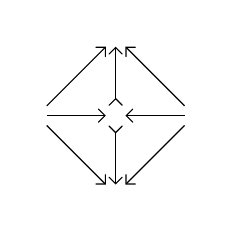
\begin{tikzpicture}
		\node (A) at (0,0) {$ $};
		\node (B) at (1,1) {$ $};
		\node (B') at (1,0) {$ $};
		\node (B'') at (1,-1) {$ $};
		\node (C) at (2,0) {$ $};
		%
		\path[->,font=\scriptsize,>=angle 90]
		(A) edge node[above]{$ $} (B)
		(A) edge node[above]{$ $} (B')
		(A) edge node[above]{$ $} (B'')
		(C) edge node[above]{$ $} (B)
		(C) edge node[above]{$ $} (B')
		(C) edge node[left]{$ $} (B'')
		(B') edge[>->] node[right]{$ $} (B)
		(B') edge[>->] node[left]{$ $} (B'');
	\end{tikzpicture}
\]

We denote this bicategory as $\bold{MonicSp(Csp(C))}$. One might wonder whether or not this condition of the inner span being monic is necessary and if a more aesthetic result is possible, but Cicala has shown that this monic condition on the spans is indeed necessary. Again, using a result of Shulman, we show that $\bold{MonicSp(Csp(C))}$ is in fact symmetric monoidal by first constructing an appropriate isofibrant symmetric monoidal double category. Furthermore, we show that the symmetric monoidal bicategory $\bold{MonicSp(Csp(C))}$ is compact closed.

The primary motivation for construction $\bimonspcsp{C}$ is the case where $\cat{C}$ is the topos $\cat{Graph}$ of (directed) graphs.  There is a symmetric monoidal compact closed sub-bicategory $\cat{Rewrite}$ of $\bimonspcsp{Graph}$ that is full on the edgeless graphs.  This should be considered as the bicategory of open graphs and all of their possible rewritings. The importance of $\cat{Rewrite}$ is that it can be used as an ambient category in which to study sub-bicategories generated from some collection of $1$-cells and $2$-cells.  We illustrate this by considering the bicategory generated by a commutative Frobenius monoid.


%%%%%%%%%%%%%%%%%%%%%%%%%%%%%%%%%%%%%%%%%%%%%%%%%%%%%%%%%%
%%%%%%%%%%%%%%%%%%%%%%%%%%%%%%%%%%%%%%%%%%%%%%%%%%%%%%%%%%
\section{Overview} % OVERVIEW
\label{sec:Overview}
%%%%%%%%%%%%%%%%%%%%%%%%%%%%%%%%%%%%%%%%%%%%%%%%%%%%%%%%%%
%%%%%%%%%%%%%%%%%%%%%%%%%%%%%%%%%%%%%%%%%%%%%%%%%%%%%%%%%%

\todo{(1) fully dualizable (2) compact closed (3) examples before and after}

Throughout, we will be working with categories with pullbacks or pushouts. Whenever we say this, we mean in particular that our category has \textit{chosen} pullbacks or pushouts.  

\begin{figure}[h]
\centering
\begin{tabular}{|ccc|}
	% Row 1
	\hline
	{2-cells} & bicategory & double category \\
	% Row 2
	\hline \hline 
	{Maps of Spans} & 
	% Maps of spans bicategory
	$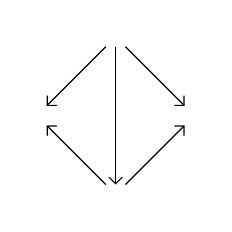
\begin{tikzpicture}
		\node (A) at (0,0) {};
		\node (B) at (1,1) {};
		\node (B') at (1,-1) {};
		\node (C) at (2,0) {};
		%
		\path[->,font=\scriptsize,>=angle 90]
		(B) edge node[above]{} (A)
		(B') edge node[above]{} (A)
		(B) edge node[above]{} (C)
		(B') edge node[above]{} (C)
		(B) edge node[left]{} (B');
	\end{tikzpicture}$ &
	% Maps of spans double category
	$\begin{tikzpicture}
		\node (A) at (0,2) {};
		\node (A') at (0,1) {};
		\node (B) at (1,2) {};
		\node (B') at (1,1) {};
		\node (C) at (2,2) {};
		\node (C') at (2,1) {};
		%
		\path[->,font=\scriptsize,>=angle 90]
		% horizontal arrows
		(B) edge node[above]{} (A)
		(B) edge node[above]{} (C)
		(B') edge node[above]{} (A')
		(B') edge node[above]{} (C')
		% vertical arrows
		(A) edge node[left]{} (A')
		(B) edge node[left]{} (B')
		(C) edge node[left]{} (C');	
	\end{tikzpicture}$ \\
	% Row 3
	\hline 
	{Maps of Cospans} &
	% maps of cospans bicategory
	$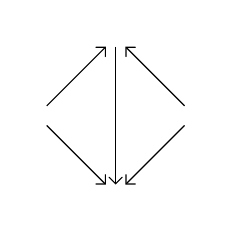
\begin{tikzpicture}
		\node (A) at (0,0) {};
		\node (B) at (1,1) {};
		\node (B') at (1,-1) {};
		\node (C) at (2,0) {};
		%
		\path[->,font=\scriptsize,>=angle 90]
		(A) edge node[above]{} (B)
		(A) edge node[above]{} (B')
		(C) edge node[above]{} (B)
		(C) edge node[above]{} (B')
		(B) edge node[left]{} (B');
	\end{tikzpicture}$ &
	% maps of cospans double category
	$\begin{tikzpicture}
		\node (A) at (0,2) {};
		\node (A') at (0,1) {};
		\node (B) at (1,2) {};
		\node (B') at (1,1) {};
		\node (C) at (2,2) {};
		\node (C') at (2,1) {};
		%
		\path[->,font=\scriptsize,>=angle 90]
		% horizontal arrows
		(A) edge node[above]{} (B)
		(C) edge node[above]{} (B)
		(A') edge node[above]{} (B')
		(C') edge node[above]{} (B')
		% vertical arrows
		(A) edge node[left]{} (A')
		(B) edge node[left]{} (B')
		(C) edge node[left]{} (C');	
	\end{tikzpicture}$\\
	% Row 4
	\hline 
	{Spans of Spans} & 
	% spans of spans bicategory
	$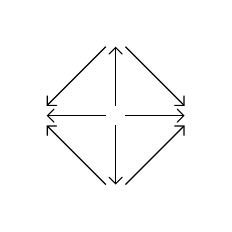
\begin{tikzpicture}
		\node (A) at (0,0) {};
		\node (B) at (1,1) {};
		\node (B') at (1,0) {};
		\node (B'') at (1,-1) {};
		\node (C) at (2,0) {};
		%
		\path[->,font=\scriptsize,>=angle 90]
		(B) edge node[above]{} (A)
		(B) edge node[above]{} (C)
		(B') edge[->] node[left]{} (A)
		(B') edge[->] node[right]{} (C)
		(B'') edge node[left]{} (A)
		(B'') edge node[left]{} (C)
		(B') edge node[left]{} (B)
		(B') edge node[right]{} (B'');
	\end{tikzpicture}$ &
	% spans of spans double category
	$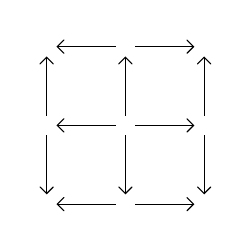
\begin{tikzpicture}
		\node (A) at (0,2) {};
		\node (A') at (0,1) {};
		\node (A'') at (0,0) {};
		\node (B) at (1,2) {};
		\node (B') at (1,1) {};
		\node (B'') at (1,0) {};
		\node (C) at (2,2) {};
		\node (C') at (2,1) {};
		\node (C'') at (2,0) {};
		%
		\path[->,font=\scriptsize,>=angle 90]
		% horizontal arrows
		(B) edge node[above]{} (A)
		(B) edge node[above]{} (C)
		(B') edge node[above]{} (A')
		(B') edge node[above]{} (C')
		(B'') edge node[above]{} (A'')
		(B'') edge node[above]{} (C'')
		% vertical arrows
		(A') edge node[left]{} (A)
		(A') edge node[left]{} (A'')
		(B') edge node[left]{} (B)
		(B') edge node[left]{} (B'')
		(C') edge node[left]{} (C)
		(C') edge node[left]{} (C'');	
	\end{tikzpicture}$\\
	% Row 5
	\hline 
	{Cospans of Copans} & 
	% cospans of cospans bicategory
	$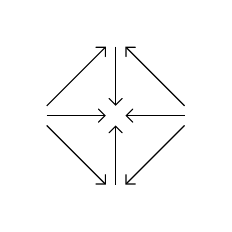
\begin{tikzpicture}
		\node (A) at (0,0) {};
		\node (B) at (1,1) {};
		\node (B') at (1,0) {};
		\node (B'') at (1,-1) {};
		\node (C) at (2,0) {};
		%
		\path[->,font=\scriptsize,>=angle 90]
		(A) edge node[above]{} (B)
		(A) edge node[above]{} (B')
		(A) edge[->] node[left]{} (B'')
		(C) edge[->] node[right]{} (B)
		(C) edge node[left]{} (B')
		(C) edge node[left]{} (B'')
		(B) edge node[left]{} (B')
		(B'') edge node[right]{} (B');
	\end{tikzpicture}$ &
	% cospans of cospans double category
	$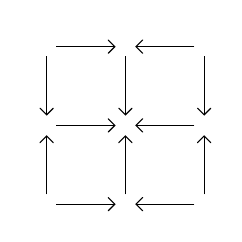
\begin{tikzpicture}
		\node (A) at (0,2) {};
		\node (A') at (0,1) {};
		\node (A'') at (0,0) {};
		\node (B) at (1,2) {};
		\node (B') at (1,1) {};
		\node (B'') at (1,0) {};
		\node (C) at (2,2) {};
		\node (C') at (2,1) {};
		\node (C'') at (2,0) {};
		%
		\path[->,font=\scriptsize,>=angle 90]
		% horizontal arrows
		(A) edge node[above]{} (B)
		(A') edge node[above]{} (B')
		(A'') edge node[above]{} (B'')
		(C) edge node[above]{} (B)
		(C') edge node[above]{} (B')
		(C'') edge node[above]{} (B'')
		% vertical arrows
		(A) edge node[left]{} (A')
		(A'') edge node[left]{} (A')
		(B) edge node[left]{} (B')
		(B'') edge node[left]{} (B')
		(C) edge node[left]{} (C')
		(C'') edge node[left]{} (C');	
	\end{tikzpicture}$ \\
	% Row 6
	\hline 
	{Monic Spans of Copans} & 
	% monic spans of cospans bicategory
	$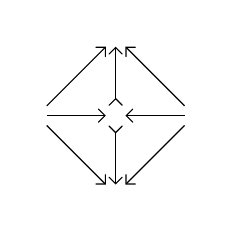
\begin{tikzpicture}
		\node (A) at (0,0) {$ $};
		\node (B) at (1,1) {$ $};
		\node (B') at (1,0) {$ $};
		\node (B'') at (1,-1) {$ $};
		\node (C) at (2,0) {$ $};
		%
		\path[->,font=\scriptsize,>=angle 90]
		(A) edge node[above]{$ $} (B)
		(A) edge node[above]{$ $} (B')
		(A) edge node[above]{$ $} (B'')
		(C) edge node[above]{$ $} (B)
		(C) edge node[above]{$ $} (B')
		(C) edge node[left]{$ $} (B'')
		(B') edge[>->] node[right]{$ $} (B)
		(B') edge[>->] node[left]{$ $} (B'');
	\end{tikzpicture}$ &
	% monic spans of cospans double category
	$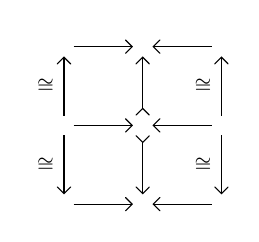
\begin{tikzpicture}
		\node (A) at (0,2) {$ $};
		\node (A') at (0,1) {$ $};
		\node (A'') at (0,0) {$ $};
		\node (B) at (1,2) {$ $};
		\node (B') at (1,1) {$ $};
		\node (B'') at (1,0) {$ $};
		\node (C) at (2,2) {$ $};
		\node (C') at (2,1) {$ $};
		\node (C'') at (2,0) {$ $};
		%
		\path[->,font=\scriptsize,>=angle 90]
		% horizontal arrows
		(A) edge node[above]{$ $} (B)
		(A') edge node[above]{$ $} (B')
		(A'') edge node[above]{$ $} (B'')
		(C) edge node[above]{$ $} (B)
		(C') edge node[above]{$ $} (B')
		(C'') edge node[above]{$ $} (B'')
		% vertical arrows
		(A') edge node[left]{$\cong$} (A)
		(A') edge node[left]{$\cong$} (A'')
		(B') edge[>->] node[left]{$ $} (B)
		(B') edge[>->] node[left]{$ $} (B'')
		(C') edge node[left]{$\cong$} (C)
		(C') edge node[left]{$\cong$} (C'');
	\end{tikzpicture}$ \\
	% Row 7
	\hline 
	{Epic Cospans of Spans} & 
	% epic cospans of spans bicategory
	$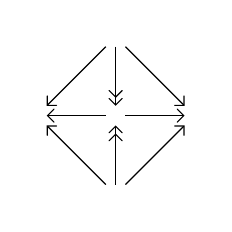
\begin{tikzpicture}
		\node (A) at (0,0) {$ $};
		\node (B) at (1,1) {$ $};
		\node (B') at (1,0) {$ $};
		\node (B'') at (1,-1) {$ $};
		\node (C) at (2,0) {$ $};
		%
		\path[->,font=\scriptsize,>=angle 90]
		(B) edge node[above]{$ $} (A)
		(B) edge node[left]{$ $} (C)
		(B') edge node[left]{$ $} (A)
		(B') edge node[right]{$ $} (C)
		(B'') edge node[left]{$ $} (A)
		(B'') edge node[left]{$ $} (C)
		(B) edge[->>] node[left]{$ $} (B')
		(B'') edge[->>] node[right]{$ $} (B');
	\end{tikzpicture}$ &
	% epic cospans of spans double category
	$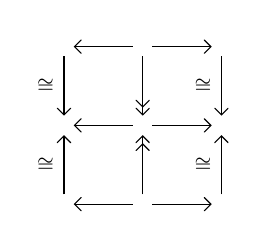
\begin{tikzpicture}
		\node (A) at (0,2) {$ $};
		\node (A') at (0,1) {$ $};
		\node (A'') at (0,0) {$ $};
		\node (B) at (1,2) {$ $};
		\node (B') at (1,1) {$ $};
		\node (B'') at (1,0) {$ $};
		\node (C) at (2,2) {$ $};
		\node (C') at (2,1) {$ $};
		\node (C'') at (2,0) {$ $};
		%
		\path[->,font=\scriptsize,>=angle 90]
		% horizontal arrows
		(B) edge node[above]{$ $} (A)
		(B) edge node[above]{$ $} (C)
		(B') edge node[above]{$ $} (A')
		(B') edge node[above]{$ $} (C')
		(B'') edge node[above]{$ $} (A'')
		(B'') edge node[above]{$ $} (C'')
		% vertical arrows
		(A) edge node[left]{$\cong$} (A')
		(A'') edge node[left]{$\cong$} (A')
		(B) edge[->>] node[left]{$ $} (B')
		(B'') edge[->>] node[left]{$ $} (B')
		(C) edge node[left]{$\cong$} (C')
		(C'') edge node[left]{$\cong$} (C');
	\end{tikzpicture}$ \\
	\hline 
\end{tabular}
\caption{Bicategory and double category 2-cells}
\label{fig:2cells}
\end{figure}


%%%%%%%%%%%%%%%%%%%%%%%%%%%%%%%%%%%%%%%%%%%%%%%%%%%%%%%%%%
%%%%%%%%%%%%%%%%%%%%%%%%%%%%%%%%%%%%%%%%%%%%%%%%%%%%%%%%%%
\section{Background} % EXAMPLES
\label{sec:Examples}
%%%%%%%%%%%%%%%%%%%%%%%%%%%%%%%%%%%%%%%%%%%%%%%%%%%%%%%%%%
%%%%%%%%%%%%%%%%%%%%%%%%%%%%%%%%%%%%%%%%%%%%%%%%%%%%%%%%%%

Here we will discuss some of the background of the various span and cospan bicategories.  Nothing here is new, but it provides a quick refresher as well as allows us to set our notation.  Throughout this paper, $\cat{C}$ will be a category with finite limits and $\cat{D}$ will be a category with finite colimits.  

One of the first examples given of a bicategory \cite{Be} is $\bispmap{C}$ whose objects are the $\cat{C}$-objects, $1$-cells $x \to z$ are given by $\cat{C}$-spans 
\[
	x \gets y \to z 
\]
which we denote by $y \from x \tospan z$ when convenient, and $2$-cells 
\[
	(y \from x \tospan z) \Rightarrow (y' \from x' \tospan z')
\] 
are given by diagrams
\[
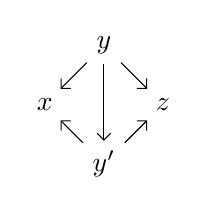
\begin{tikzpicture}
	\node (A) at (0,0) {$x$};
	\node (B) at (0.75,0.75) {$y$};
	\node (B') at (0.75,-0.75) {$y'$};
	\node (C) at (1.5,0) {$z$};
	%
	\path[->,font=\scriptsize,>=angle 90]
	(B) edge node[above]{$ $} (A)
	(B') edge node[above]{$ $} (A)
	(B) edge node[above]{$ $} (C)
	(B') edge node[above]{$ $} (C)
	(B) edge node[left]{$ $} (B');
\end{tikzpicture}
\]
There is a similar category denoted $\bicspmap{D}$ consisting of $\cat{D}$-objects, $\cat{D}$-cospans which we denote $y \from x \tocospan z$, and maps of $\cat{D}$-cospans given by diagrams  
\[
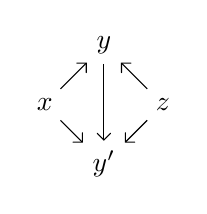
\begin{tikzpicture}
	\node (A) at (0,0) {$x$};
	\node (B) at (0.75,0.75) {$y$};
	\node (B') at (0.75,-0.75) {$y'$};
	\node (C) at (1.5,0) {$z$};
	%
	\path[->,font=\scriptsize,>=angle 90]
	(A) edge node[above]{$ $} (B)
	(A) edge node[above]{$ $} (B')
	(C) edge node[above]{$ $} (B)
	(C) edge node[above]{$ $} (B')
	(B) edge node[left]{$ $} (B');
\end{tikzpicture}
\]

% EXAMPLE: COREL
%
We can capture the notions of relations and corelations with these sort of bicategories. First, recall the definitions of jointly monic and jointly epic.  A span $x \gets y \to z$ is called \emph{jointly monic} if the pairing $y \to x \times z$ is monic.  A cospan $x \to y \gets z$ is called \emph{jointly epic} if the copairing $x+z \to y$ is epic. A relation $X \nrightarrow Y$ between sets $X$ and $Y$ is a subobject $R$ of $X \times Y$. It is well-known that a relation of sets is simply a jointly monic span $\cat{Set}$.  The dual notion is called a corelation. The usefulness of corelations were discussed by Coya and Fong in \cite{CoyaFong} as well as by Bruni and Gadducci in \cite{BruniGadducci} under the alias `equivalence relation'.  

\begin{ex}
	A \emph{corelation} between objects $X$ and $Y$ of a category is a co-subobject of $X+Y$, or rather an equivalence class of epimorphisms $X+Y \to C$ for some object $C$. Taking finite sets and corelations between them gives a symmetric monoidal category $\cat{Corel}$.  Set theoretically, a corelation $C \from X \nrightarrow Y$  is simply an equivalence relation on $X+Y$ given by taking the fibers of the surjection $X+Y \to C$. We get an category $\bispmap{FinSet}_{\text{JE}}$ equivalent to $\cat{Corel}$ by taking the subcategory of finite sets and cospans consisting of all objects and jointly epic cospans.  We can promote $\bispmap{FinSet}_{\text{JE}}$ to a bicategory by defining $\bispmap{FinSet}_{\text{JE}}(X,Y)$ to consist of all maps of cospans. Hence $\bispmap{FinSet}_{\text{JE}}(X,Y)$ is equivalent to the full subcategory of the over-category $X+Y/\cat{FinSet}$ whose objects are the surjective maps $X+Y \to C$. So a $2$-cell in $\bispmap{FinSet}_{\text{JE}}$ is really just a commuting diagram
	\[
	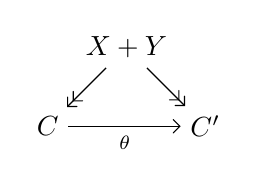
\begin{tikzpicture}
		\node (A) at (0,1) {$X+Y$};
		\node (B) at (-1,0) {$C$};
		\node (C) at (1,0) {$C'$};
		%
		\path[->,font=\scriptsize,>=angle 90]
		(A) edge[->>] node[above]{$$} (B)
		(A) edge[->>] node[above]{$$} (C)
		(B) edge node[below]{$\theta$} (C);
	\end{tikzpicture}
	\]
	Note that $\bispmap{FinSet}_{\text{JE}}(X,Y)$ is locally posetal -- that is if $\theta$ does exist, it is the unique $2$-cell $C \Rightarrow C'$.  Indeed, for $c \in C$, the fiber of $c$ is contained in the fiber of $\theta (c)$ meaning that $\theta$ is completely determined by the corelations.  Inspiration now leads us to promote $\cat{Corel}$ to a bicategory by inserting a $2$-cell
	\[
	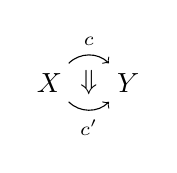
\begin{tikzpicture}
		\node (X) at (0,0) {$X$};
		\node (Y) at (1,0) {$Y$};
		%
		\path[->,font=\scriptsize]
		(X) edge[out=45,in=135] node[above]{$c$} (Y)
		(X) edge[out=-45,in=-135] node[below]{$c'$} (Y);
		%
		\node () at (0.5,0) {$\Downarrow$};
	\end{tikzpicture}
	\]
	whenever the equivalence relation given by $c$ is contained in that given by $c'$. There is an obvious biequivalence between $\cat{Corel}$ and $\bispmap{FinSet}_{\text{JE}}$. Hence $\cat{Corel}$ is a bicategory of cospans.
\end{ex}

% EXAMPLE: LIN REL
%
\begin{ex}
	The category $\cat{LinRel}$ of finite dimensional vector spaces and linear relations (subspaces of $V \oplus W$) plays an important role in network theory \cite{BaezErbele_CatControl,FongSobocRap}. As in Fong's thesis \cite{Fong_Thesis},
	we can identify $\cat{LinRel}$ with the subcategory of the category $\bispmap{FinVec}$ containing all finite dimensional vector spaces and jointly monic spans. The idea is that a jointly monic span $L \from V \tospan W$ gives an injection $L \to V \oplus W$, hence a linear relation $L \from V \nrightarrow W$. Consider the full sub-bicategory $\bispmap{FinVec}_{\text{JM}}$ of $\bispmap{FinVec}$ with all finite dimensional vector spaces and jointly monic spans. Similar to the previous example, the category $\bispmap{FinVec}_{\text{JM}}(V,W)$ is equivalent to the full subcategory of the over-category $\bispmap{FinVec}_{\text{JM}}/V \oplus W$ consisting of monics $L \to V \oplus W$.  Thus, a $2$-cell can be thought of as the diagram
	\[
	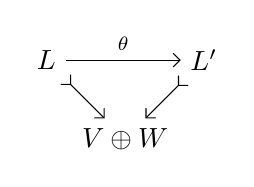
\begin{tikzpicture}
		\node (A) at (0,0) {$V \oplus W$};
		\node (B) at (-1,1) {$L$};
		\node (C) at (1,1) {$L'$};
		%
		\path[->,font=\scriptsize,>=angle 90]
		(B) edge[>->] node[above]{} (A)
		(C) edge[>->] node[above]{} (A)
		(B) edge node[above]{$\theta$} (C);
	\end{tikzpicture}
	\]
	It is easy to see that $\theta$ is monic and is the unique such morphism making these diagrams commute, assuming that it exists. As above, we promote $\cat{LinRel}$ to a bicategory by introducing a $2$-cell 
	\[
	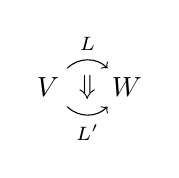
\begin{tikzpicture}
		\node (V) at (0,0) {$V$};
		\node (W) at (1,0) {$W$};
		%
		\path[->,font=\scriptsize]
		(V) edge[out=45,in=135] node[above]{$L$} (W)
		(V) edge[out=-45,in=-135] node[below]{$L'$} (W);
		%
		\node () at (0.5,0) {$\Downarrow$};
	\end{tikzpicture}
	\]
	whenever $L \subseteq L'$.  Hence, $\cat{LinRel}$ is a bicategory of spans. \todo{Make a connection to the bicategory of relations idea by carboni and Walters}
\end{ex}

Another way of promoting (co)span categories to bicategories is to consider different $2$-cells.  For example, Rebro \cite{Reb} constructed a bicategory $\bispsp{C}$ with $\cat{C}$-objects, $\cat{C}$-spans, and isomorphism classes of $\cat{C}$-spans of spans, which are diagrams of the form
\[
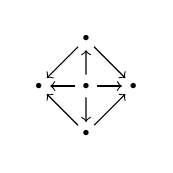
\begin{tikzpicture}[scale=0.6]
	\node[CDnode] (A) at (0,0) {$\bullet$};
	\node[CDnode] (B) at (1,1) {$\bullet$};
	\node[CDnode] (B') at (1,0) {$\bullet$};
	\node[CDnode] (B'') at (1,-1) {$\bullet$};
	\node[CDnode] (C) at (2,0) {$\bullet$};
	%
	\path[->,font=\scriptsize]
	(B) edge node[above]{$$} (A)
	(B) edge node[above]{$$} (C)
	(B') edge[->] node[left]{$$} (A)
	(B') edge[->] node[right]{$$} (C)
	(B'') edge node[left]{$$} (A)
	(B'') edge node[left]{$$} (C)
	(B') edge node[left]{$$} (B)
	(B') edge node[right]{$$} (B'');
\end{tikzpicture}
\]
Actually, the above diagram is an equivalence class of $2$-cells where we say $2$-cells are isomorphic if there is a $\cat{C}$-isomorphism $\theta$ such that
\[
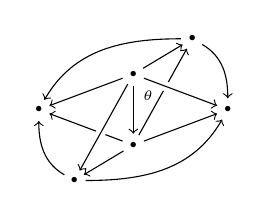
\begin{tikzpicture}[scale=0.6]
	\node[CDnode] (X) at (-2,0) {$\bullet$};
	\node[CDnode] (L) at (1.25,1.5) {$\bullet$};
	\node[CDnode] (Y) at (2,0) {$\bullet$};
	\node[CDnode] (S) at (-1.25,-1.5) {$\bullet$};
	\node[CDnode] (S'1) at (0,0.75) {$\bullet$};
	\node[CDnode] (S'2) at (0,-0.75) {$\bullet$};
	%
	\draw [<-] (X) edge[in=180,out=60] (L);
	\draw [<-] (X) edge[] (S'1);
	\draw [<-] (X) edge[] (S'2);
	\draw [<-] (X) edge[out=-90,in=150] (S);
	\draw [<-] (Y) edge[out=90,in=-30] (L);
	\draw [<-] (Y) edge[] (S'2);
	\draw [<-] (Y) edge[out=-120,in=0] (S);
	\draw [->] (S'1) edge[] (L);
	\draw [->] (S'1) edge[white,line width=3.5pt] (S);
	\draw [->] (S'1) edge[] (S);
	\draw [->] (S'1) edge node[right,pos=0.2,font=\tiny]{$\theta$} (S'2);
	\draw [->] (S'2) edge[] (L);
	\draw [->] (S'2) edge[] (S);
	\draw [<-] (Y) edge[white,line width=3.5pt] (S'1);
	\draw [<-] (Y) edge[] (S'1);
\end{tikzpicture}
\]
Similarly, there is a dual bicategory $\bicspcsp{D}$ with $\cat{D}$-objects, $\cat{D}$-cospans, and isomorphism classes $\cat{D}$-cospans of cospans

\todo{fibrations of groupoids example here}

When studying intercategories, Grandis and Par\'{e} \cite{GranPare_Intercats} looked at spans of cospans and found a lax interchange law. It was eventually shown that, under certain conditions, the interchange law is invertible \cite{Cic}. That is, while restricting attention to a topoi $\cat{T}$, there is a bicategory $\bimonspcsp{T}$ with $\cat{T}$-objects, $\cat{T}$-cospans, and isomorphism classes of monic $\cat{T}$-spans of cospans. These $2$-cells are depicted as
\[
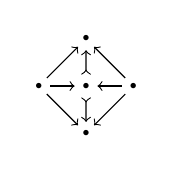
\begin{tikzpicture}[scale=.6]
	\node[CDnode] (A) at (0,0) {$\bullet$};
	\node[CDnode] (B) at (1,1) {$\bullet$};
	\node[CDnode] (B') at (1,0) {$\bullet$};
	\node[CDnode] (B'') at (1,-1) {$\bullet$};
	\node[CDnode] (C) at (2,0) {$\bullet$};
	%
	\path[->,font=\scriptsize]
	(A) edge node[above]{$ $} (B)
	(A) edge node[above]{$ $} (B')
	(A) edge node[above]{$ $} (B'')
	(C) edge node[above]{$ $} (B)
	(C) edge node[above]{$ $} (B')
	(C) edge node[left]{$ $} (B'')
	(B') edge[>->] node[right]{$ $} (B)
	(B') edge[>->] node[left]{$ $} (B'');
\end{tikzpicture}
\]
There is a dual bicategory $\biepiccspsp{T}$ with $\cat{T}$-objects, $\cat{T}$-spans, and isomorphism classes of epic $\cat{T}$-cospans of spans 

\begin{ex}
\label{ex:Rewrite}
	In \cite{Cic}, the bicategory $\cat{Rewrite}$ is introduced. This is the full sub-bicategory of $\bimonspcsp{Graph}$ with edgeless graphs for $0$-cells.  The $1$-cells are graphs with inputs and outputs chosen by the feet of the cospans.  An example of such a $1$-cell is
	\[
	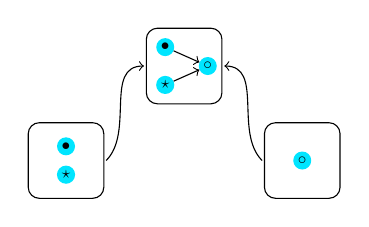
\begin{tikzpicture}[scale=.6]
		\draw[rounded corners] (-0.8,1.7) rectangle (0.8,3.3);
		\draw[rounded corners] (4.2,1.7) rectangle (5.8,3.3);
		\draw[rounded corners] (1.7,3.7) rectangle (3.3,5.3);
		%
		\node[rewritenode] (ai) at (0,2.8) {$\bullet$};
		\node[rewritenode] (bi) at (0,2.2) {$\star$};
		\node[rewritenode] (co) at (5,2.5) {$\circ$};
		\node[rewritenode] (a1) at (2.1,4.9) {$\bullet$};
		\node[rewritenode] (b1) at (2.1,4.1) {$\star$};
		\node[rewritenode] (c1) at (3,4.5) {$\circ$};
		%
		\draw [->] (a1) edge (c1);
		\draw [->] (b1) edge (c1);
		%
		\path [->] (0.85,2.5) edge[out=45,in=180] (1.65,4.5);
		\path [->] (4.15,2.5) edge[out=135,in=0] (3.35,4.5);
	\end{tikzpicture}
	\]
	which has input nodes `$\bullet$' and `$\star$' and output node `$\circ$'. Later, this $1$-cell will be the multiplication of a Frobenius algebra object. Each $2$-cell of $\cat{Rewrite}$ is a rewriting of one graph to another so that inputs and outputs are preserved. For instance, we will later present the monoid unit law as a $2$-cell
	\begin{equation}
	\label{diag:MonoidUnit}
	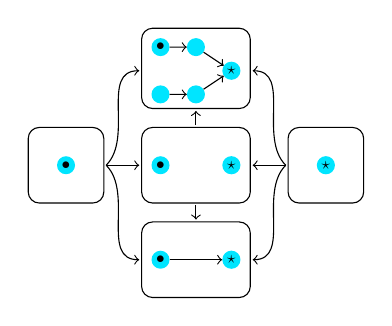
\begin{tikzpicture}[baseline=(current  bounding  box.center),scale=.6]
		\draw[rounded corners] (1.6,-0.3) rectangle (3.9,1.3);
		\draw[rounded corners] (1.6,1.7) rectangle (3.9,3.3);
		\draw[rounded corners] (1.6,3.7) rectangle (3.9,5.4);
		\draw[rounded corners] (-0.8,1.7) rectangle (0.8,3.3);
		\draw[rounded corners] (4.7,1.7) rectangle (6.3,3.3);
		%
		\node[rewritenode] (ai) at (0,2.5) {$\bullet$};
		\node[rewritenode] (bo) at (5.5,2.5) {$\star$};
		\node[rewritenode] (a1) at (2,5) {$\bullet$};
		\node[rewritenode] (b1) at (2.75,5) {$\bluebullet$};
		\node[rewritenode] (c1) at (2,4) {$\bluebullet$};
		\node[rewritenode] (d1) at (2.75,4) {$\bluebullet$};
		\node[rewritenode] (e1) at (3.5,4.5) {$\star$};
		\node[rewritenode] (a2) at (2,2.5) {$\bullet$};
		\node[rewritenode] (b2) at (3.5,2.5) {$\star$};
		\node[rewritenode] (a3) at (2,0.5) {$\bullet$};
		\node[rewritenode] (b3) at (3.5,0.5) {$\star$};
		%
		\draw [->] (a1) edge (b1);
		\draw [->] (b1) edge (e1);
		\draw [->] (c1) edge (d1);
		\draw [->] (d1) edge (e1);
		\draw [->] (a3) edge (b3);
		%
		\path [->] (0.85,2.5) edge[out=0,in=180] (1.55,2.5);
		\path [->] (0.85,2.5) edge[out=45,in=180] (1.55,4.5);
		\path [->] (0.85,2.5) edge[out=-45,in=180] (1.55,0.5);
		\path [->] (4.65,2.5) edge[out=180,in=0] (3.95,2.5);
		\path [->] (4.65,2.5) edge[out=135,in=0] (3.95,4.5);
		\path [->] (4.65,2.5) edge[out=225,in=0] (3.95,0.5);
		\draw [->] (2.75,3.35) -- (2.75,3.65);
		\draw [->] (2.75,1.65) -- (2.75,1.35);
	\end{tikzpicture}
	\end{equation}
\end{ex}

\todo{List of conventions: define $\nabla$, using $X$ for identity on $X$, $\tocospan$ arrow,bicategory}

%%%%%%%%%%%%%%%%%%%%%%%%%%%%%%%%%%%%%%%%%%%%%%%%%%%%%%%%%%
%%%%%%%%%%%%%%%%%%%%%%%%%%%%%%%%%%%%%%%%%%%%%%%%%%%%%%%%%%
\section{Double categories and duality} % DOUBLE CATS AND DUALITY SECTION
\label{sec:DoubleCategories}
%%%%%%%%%%%%%%%%%%%%%%%%%%%%%%%%%%%%%%%%%%%%%%%%%%%%%%%%%%
%%%%%%%%%%%%%%%%%%%%%%%%%%%%%%%%%%%%%%%%%%%%%%%%%%%%%%%%%%

Nothing in this section is new, but we will use the results presented here in showing that the span and cospan bicategories from the previous section have symmetric monoidal and duality structures. The first subsection on double categories closely follows \cite{Shul}.  The second section discusses duality in bicategories. The material contained there can be found in \cite{Lurie,Piotr,Stay}.

%%%%%%%%%%%%%%%%%%%%%%%%%%%%%%%%%%%%%%%%%%%%%%%%%%%%%%%%%%
\subsection{Monoidal bicategories via double categories} % DOUBLE CATS
\label{subsec:DoubleCategories}
%%%%%%%%%%%%%%%%%%%%%%%%%%%%%%%%%%%%%%%%%%%%%%%%%%%%%%%%%%

Pseudo double categories, also known as weak double categories or just double categories, have been studied by Fiore in \cite{Fiore} and Par\'{e} and Grandis in \cite{Gran}. Before formally defining them, it is helpful to have the following picture in mind. A pseudo double category has $2$-morphisms shaped like

\begin{equation}
\label{diag:DblCatSquare}
\raisebox{-0.5\height}{
	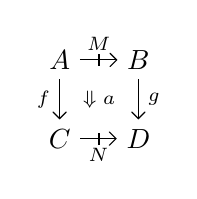
\begin{tikzpicture}
	\node (A) at (0,1) {$A$};
	\node (B) at (1,1) {$B$};
	\node (C) at (0,0) {$C$};
	\node (D) at (1,0) {$D$};
	%
	\path[->,font=\scriptsize,>=angle 90]
	(A) edge node[above]{$M$} (B)
	(A) edge node[left]{$f$} (C)
	(B) edge node[right]{$g$} (D)
	(C) edge node[below]{$N$} (D);
	%
	\draw (0.5,.925) -- (0.5,1.075);
	\draw (0.5,-.075) -- (0.5,.075);
	\node () at (0.5,0.5) {\scriptsize{$\Downarrow a$}};
	\end{tikzpicture}
}
\end{equation}

We call $A, B, C$ and $D$ objects or \emph{0-cells}, $f$ and $g$ \emph{vertical 1-cells}, $M$ and $N$ \emph{horizontal 1-cells} and $a$ a \emph{2-cells}. Note that a \emph{vertical 1-cell} is a morphism between \emph{0-cells} and a \emph{2-cell} is a morphism between \emph{horizontal 1-cells}. We will denote both kinds of morphisms and horizontal 1-cells as a single arrow, namely `$\to$', unless in a diagram, in which case they will be denoted as above.

We follow the notation of Shulman \cite{Shul} with the following definitions.

% DEFINITION -- Double Category
%
\begin{defn}
	\label{def:DoubleCategory}
	A \emph{pseudo double category} $\dblcat{D}$, or simply \emph{double category}, consists of a category of objects $\dblcat{D}_{0}$ and a category of arrows $\dblcat{D}_{1}$ with the following functors
	\begin{equation*}
	\begin{split}
	U & \from \dblcat{D}_{0} \to \dblcat{D}_{1}, \\
	S,T & \from \dblcat{D}_{1} \rightrightarrows \dblcat{D}_{0}, \t{ and} \\
	\odot & \from \dblcat{D}_{1} \times_{\dblcat{D}_{0}} \dblcat{D}_{1} \to \dblcat{D}_{1}
	\end{split}
	\end{equation*}
	where the pullback $\dblcat{D}_{1} \times_{\dblcat{D}_{0}} \dblcat{D}_{1}$ is taken over $S$ and $T$.  These functors satisfy the equations
	\begin{equation*}
	\begin{split}
	S(U_{A}) = A &= T(U_{A}) \\
	S(M \odot N) & = SN \\
	T(M \odot N) & = TM. 
	\end{split}
	\end{equation*}
	This also comes equipped with natural isomorphisms
	\begin{equation*}
	\begin{split}
	\alpha & \from (M \odot N) \odot P \to M \odot (N \odot P)\\
	\lambda & \from U_{B} \odot M \to M\\
	\rho & \from M \odot U_{A} \to M
	\end{split}
	\end{equation*}
	such that $S(\alpha)$, $S(\lambda)$, $S(\rho)$, $T(\alpha)$, $T(\lambda)$, and $T(\rho)$ are all identities and that the coherence axioms of a monoidal category are satisfied. 
	
	Objects of $\dblcat{D}_{0}$ are called \emph{$0$-cells} and morphisms of $\dblcat{D}_{0}$ are called \emph{vertical $1$-cells}. Objects of $\dblcat{D}_{1}$ are called \emph{horizontal $1$-cells} and morphisms of $\dblcat{D}_{1}$ are called \emph{$2$-cells}. The morphisms of $\dblcat{D}_{0}$, which are the vertical $1$-cells, will be denoted $f \colon A \to C$ and we denote a 1-cell $M$ with $S(M)=A,T(M)=B$ by $M \colon A \hto B$. Then a 2-cell $a \colon M \to N$ of $\dblcat{D}_{1}$ with $S(a)=f$, $T(a)=g$ would look like
	\begin{equation}
	\label{eq:square}
	\raisebox{-0.5\height}{
		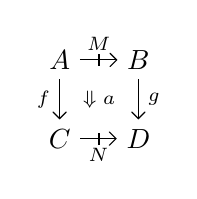
\begin{tikzpicture}
		\node (A) at (0,1) {$A$};
		\node (B) at (1,1) {$B$};
		\node (C) at (0,0) {$C$};
		\node (D) at (1,0) {$D$};
		%
		\path[->,font=\scriptsize,>=angle 90]
		(A) edge node[above]{$M$} (B)
		(A) edge node[left]{$f$} (C)
		(B) edge node[right]{$g$} (D)
		(C) edge node[below]{$N$} (D);
		%
		\draw (0.5,.925) -- (0.5,1.075);
		\draw (0.5,-.075) -- (0.5,.075);
		\node () at (0.5,0.5) {\scriptsize{$\Downarrow a$}};
		\end{tikzpicture}
	}
	\end{equation}
\end{defn}

The key difference between a \emph{strict} double category and a pseudo double category is that in a pseudo double category, horizontal composition is associative and unital only up to natural isomorphism. Equivalently, as a double category can be viewed as a category internal to $\cat{Cat}$, we can view a pseudo double category as a category \emph{weakly} internal to $\cat{Cat}$. We will sometimes omit the word pseudo and simply say double category.

\begin{defn}
	A 2-morphism where $f$ and $g$ are identities is called a \emph{globular 2-morphism}.
\end{defn}

\begin{defn}
	Let $\dblcat{D}$ be a pseudo double category. Then the \emph{horizontal edge bicategory} of $\dblcat{D}$, which we denote as $H(\dblcat{D})$, is the bicategory consisting of objects of $\dblcat{D}$, 1-morphisms that are horizontal 1-cells of $\dblcat{D}$ and 2-morphisms that are globular 2-morphisms.
\end{defn}

% DEFINITION -- Monoidal Double Category
%
\begin{defn}
	\label{def:MonoidalDoubleCategory}
	A \textbf{monoidal double category} is a double category $\dblcat{D}$ equipped the following
	structure.
	\begin{enumerate}
		\item $\dblcat{D}_{0}$ and $\dblcat{D}_{1}$ are both monoidal categories.
		%
		\item If $I$ is the monoidal unit of $\dblcat{D}_{0}$, then $U_I$ is the
		monoidal unit of $\dblcat{D}_{1}$.
		%
		\item The functors $S$ and $T$ are strict monoidal, that is $S(M \otimes N)
		= SM \otimes SN$ and $T(M \otimes N)=TM \otimes TN$ and $S$ and $T$ also
		preserve the associativity and unit constraints.
		%
		\item We have globular isomorphisms
		\[ 
		\mathfrak{x} \from 
		(M_1 \otimes N_1) \odot (M_2 \otimes N_2) 
		\to 
		(M_1\odot M_2) \otimes (N_1\odot N_2)
		\]
		and
		\[
		\mathfrak{u} \from U_{A \otimes B} \to (U_A \otimes U_B)
		\]
		such that the following diagrams commute:
		\[
		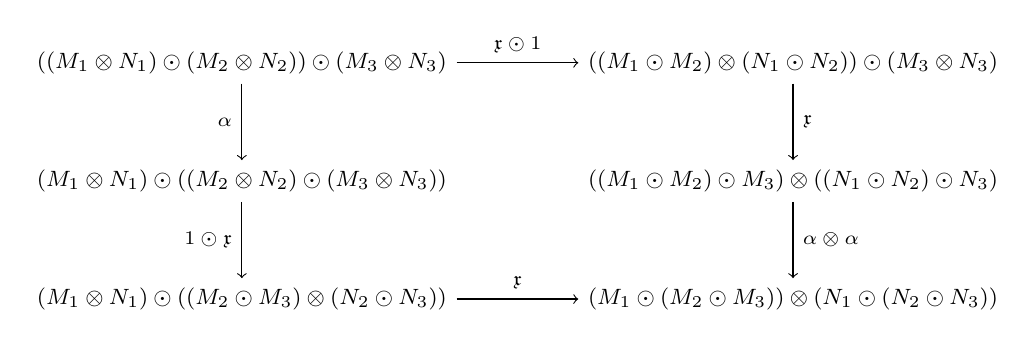
\begin{tikzpicture}
		\node (A) at (0,3) {\footnotesize{$((M_1\otimes N_1)\odot (M_2\otimes N_2)) \odot (M_3\otimes N_3)$}};
		\node (B) at (7,3) {\footnotesize{$((M_1\odot M_2)\otimes (N_1\odot N_2)) \odot (M_3\otimes N_3) $}};
		\node (A') at (0,1.5) {\footnotesize{$(M_1\otimes N_1)\odot ((M_2\otimes N_2) \odot (M_3\otimes N_3)) $}};
		\node (B') at (7,1.5) {\footnotesize{$((M_1\odot M_2)\odot M_3) \otimes ((N_1\odot N_2)\odot N_3)$}};
		\node (A'') at (0,0) {\footnotesize{$(M_1\otimes N_1) \odot ((M_2\odot M_3) \otimes (N_2\odot N_3))$}};
		\node (B'') at (7,0) {\footnotesize{$(M_1\odot (M_2\odot M_3)) \otimes (N_1\odot (N_2\odot N_3))$}};
		%
		\path[->,font=\scriptsize]
		(A) edge node[left]{$\alpha$} (A')
		(A') edge node[left]{$1 \odot \mathfrak{x}$} (A'')
		(B) edge node[right]{$\mathfrak{x}$} (B')
		(B') edge node[right]{$\alpha \otimes \alpha$} (B'')
		(A) edge node[above]{$\mathfrak{x} \odot 1$} (B)
		(A'') edge node[above]{$\mathfrak{x}$} (B'');
		\end{tikzpicture}
		\]
		\[
		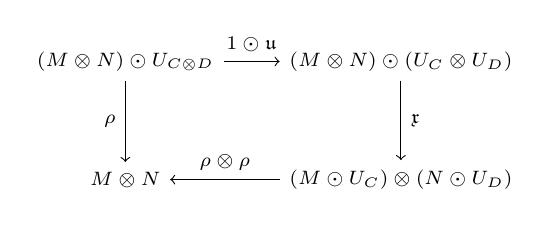
\begin{tikzpicture}
		\node (UL) at (0,1.5) {\scriptsize{$(M\otimes N) \odot U_{C\otimes D}$}};
		\node (LL) at (0,0) {\scriptsize{$M\otimes N$}};
		\node (UR) at (3.5,1.5) {\scriptsize{$(M\otimes N)\odot (U_C\otimes U_D)$}};
		\node (LR) at (3.5,0) {\scriptsize{$(M\odot U_C) \otimes (N\odot U_D)$}};
		%
		\path[->,font=\scriptsize]
		(UL) edge node[above]{$1 \odot \mathfrak{u}$} (UR) 
		(UL) edge node[left]{$\rho$} (LL)
		(LR) edge node[above]{$\rho \otimes \rho$} (LL)
		(UR) edge node[right]{$\mathfrak{x}$} (LR);
		\end{tikzpicture}
		%
		\quad
		%
		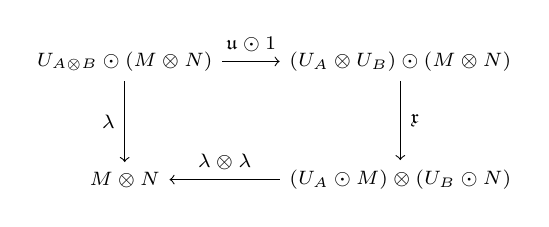
\begin{tikzpicture}
		\node (UL) at (0,1.5) {\scriptsize{$U_{A\otimes B}\odot (M\otimes N)$}};
		\node (LL) at (0,0) {\scriptsize{$M\otimes N$}};
		\node (UR) at (3.5,1.5) {\scriptsize{$(U_A\otimes U_B)\odot (M\otimes N)$}};
		\node (LR) at (3.5,0) {\scriptsize{$(U_A \odot M) \otimes (U_B\odot N)$}};
		%
		\path[->,font=\scriptsize]
		(UL) edge node[above]{$\mathfrak{u} \odot 1$} (UR) 
		(UL) edge node[left]{$\lambda$} (LL)
		(LR) edge node[above]{$\lambda \otimes \lambda$} (LL)
		(UR) edge node[right]{$\mathfrak{x}$} (LR);
		\end{tikzpicture}
		\]
		%
		\item The following diagrams commute, expressing that the
		associativity isomorphism for $\otimes$ is a transformation of double
		categories.
		\[
		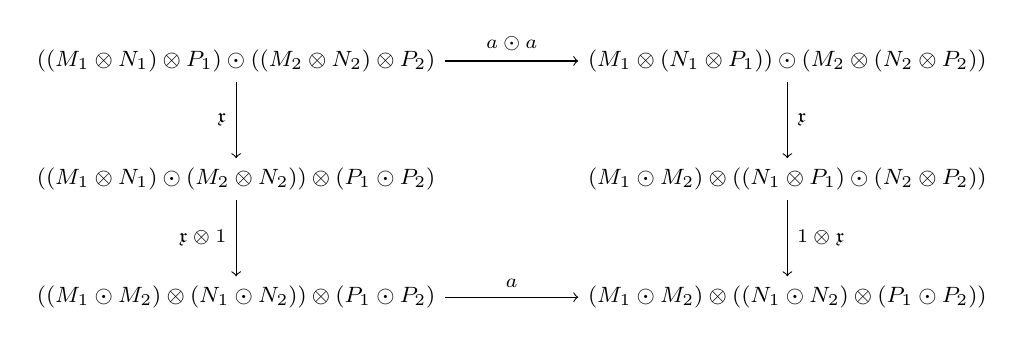
\begin{tikzpicture}
		\node (A) at (0,3) {\footnotesize{$((M_1\otimes N_1)\otimes P_1) \odot ((M_2\otimes N_2)\otimes P_2)$}};
		\node (B) at (7,3) {\footnotesize{$(M_1\otimes (N_1\otimes P_1)) \odot (M_2\otimes (N_2\otimes P_2))$}};
		\node (A') at (0,1.5) {\footnotesize{$((M_1\otimes N_1) \odot (M_2\otimes N_2)) \otimes (P_1\odot P_2)$}};
		\node (B') at (7,1.5) {\footnotesize{$(M_1\odot M_2) \otimes ((N_1\otimes P_1)\odot (N_2\otimes P_2))$}};
		\node (A'') at (0,0) {\footnotesize{$((M_1\odot M_2) \otimes(N_1\odot N_2)) \otimes (P_1\odot P_2)$}};
		\node (B'') at (7,0) {\footnotesize{$(M_1\odot M_2) \otimes ((N_1\odot N_2)\otimes (P_1\odot P_2))$}};
		%
		\path[->,font=\scriptsize]
		(A) edge node[left]{$\mathfrak{x}$} (A')
		(A') edge node[left]{$\mathfrak{x} \otimes 1$} (A'')
		(B) edge node[right]{$\mathfrak{x}$} (B')
		(B') edge node[right]{$1 \otimes \mathfrak{x}$} (B'')
		(A) edge node[above]{$a \odot a$} (B)
		(A'') edge node[above]{$a$} (B'');
		\end{tikzpicture}
		\]
		\[
		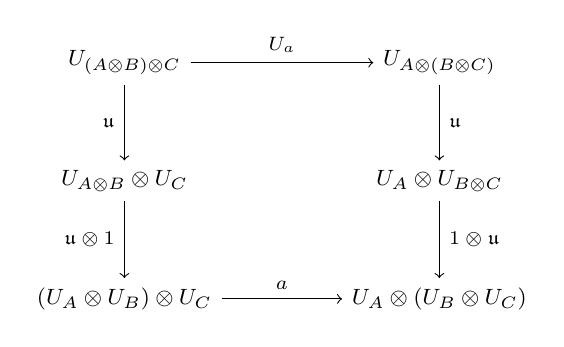
\begin{tikzpicture}
		\node (A) at (0,3) {\footnotesize{$U_{(A\otimes B)\otimes C}$}};
		\node (B) at (4,3) {\footnotesize{$U_{A\otimes (B\otimes C)} $}};
		\node (A') at (0,1.5) {\footnotesize{$U_{A\otimes B} \otimes U_C $}};
		\node (B') at (4,1.5) {\footnotesize{$U_A\otimes U_{B\otimes C}$}};
		\node (A'') at (0,0) {\footnotesize{$(U_A\otimes U_B)\otimes U_C$}};
		\node (B'') at (4,0) {\footnotesize{$U_A\otimes (U_B\otimes U_C) $}};
		%
		\path[->,font=\scriptsize]
		(A) edge node[left]{$\mathfrak{u}$} (A')
		(A') edge node[left]{$\mathfrak{u} \otimes 1$} (A'')
		(B) edge node[right]{$\mathfrak{u}$} (B')
		(B') edge node[right]{$1 \otimes \mathfrak{u}$} (B'')
		(A) edge node[above]{$U_{a}$} (B)
		(A'') edge node[above]{$a$} (B'');
		\end{tikzpicture}
		\]
		\item The following diagrams commute, expressing that the unit
		isomorphisms for $\otimes$ are transformations of double categories.
		\[
		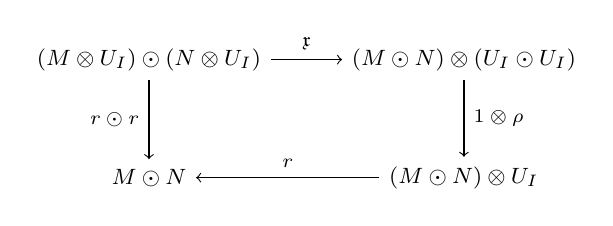
\begin{tikzpicture}
		\node (A) at (0,1.5) {\footnotesize{$(M\otimes U_I)\odot (N\otimes U_I)$}};
		\node (A') at (0,0) {\footnotesize{$M\odot N $}};
		\node (B) at (4,1.5) {\footnotesize{$(M\odot N)\otimes (U_I \odot U_I) $}};
		\node (B') at (4,0) {\footnotesize{$(M\odot N)\otimes U_I $}};
		%
		\path[->,font=\scriptsize]
		(A) edge node[left]{$r \odot r$} (A')
		(A) edge node[above]{$\mathfrak{x}$} (B)
		(B) edge node[right]{$1 \otimes \rho$} (B')
		(B') edge node[above]{$r$} (A');
		\end{tikzpicture}
		%
		\quad
		%
		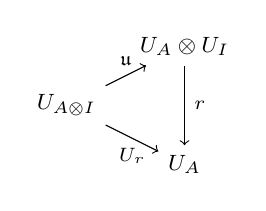
\begin{tikzpicture}
		\node (A) at (0,0.75) {\footnotesize{$U_{A\otimes I} $}};
		\node (B) at (1.5,1.5) {\footnotesize{$U_A\otimes U_I $}};
		\node (B') at (1.5,0) {\footnotesize{$U_A$}};
		%
		\path[->,font=\scriptsize]
		(A) edge node[above]{$\mathfrak{u}$} (B)
		(A) edge node[below]{$U_{r}$} (B')
		(B) edge node[right]{$r$} (B');
		\end{tikzpicture}
		\]
		%
		%
		%
		%
		\[
		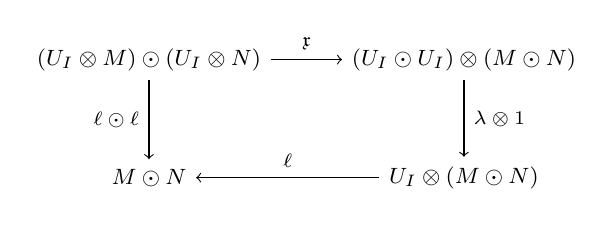
\begin{tikzpicture}
		\node (A) at (0,1.5) {\footnotesize{$(U_I\otimes M)\odot (U_I\otimes N)$}};
		\node (A') at (0,0) {\footnotesize{$M\odot N$}};
		\node (B) at (4,1.5) {\footnotesize{$(U_I \odot U_I) \otimes (M\odot N)$}};
		\node (B') at (4,0) {\footnotesize{$U_I\otimes (M\odot N) $}};
		%
		\path[->,font=\scriptsize]
		(A) edge node[left]{$\ell \odot \ell$} (A')
		(A) edge node[above]{$\mathfrak{x}$} (B)
		(B) edge node[right]{$\lambda \otimes 1$} (B')
		(B') edge node[above]{$\ell$} (A');
		\end{tikzpicture}
		%
		\quad
		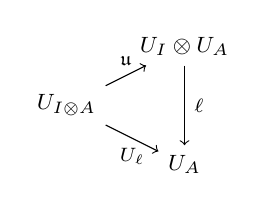
\begin{tikzpicture}
		\node (A) at (0,0.75) {\footnotesize{$U_{I\otimes A}$}};
		\node (B) at (1.5,1.5) {\footnotesize{$U_I\otimes U_A$}};
		\node (B') at (1.5,0) {\footnotesize{$U_A$}};
		%
		\path[->,font=\scriptsize]
		(A) edge node[above]{$\mathfrak{u}$} (B)
		(A) edge node[below]{$U_{\ell}$} (B')
		(B) edge node[right]{$\ell$} (B');
		\end{tikzpicture}
		\]
		\newcounter{mondbl}
		\setcounter{mondbl}{\value{enumi}}
	\end{enumerate}
	Similarly, a braided monoidal double category is a monoidal double
	category with the following additional structure.
	\begin{enumerate}
		\setcounter{enumi}{\value{mondbl}}
		\item $\dblcat{D}_{0}$ and $\dblcat{D}_{1}$ are braided monoidal categories.
		%
		\item The functors $S$ and $T$ are strict braided monoidal.
		%
		\item The following diagrams commute, expressing that the braiding is
		a transformation of double categories.
		\[
		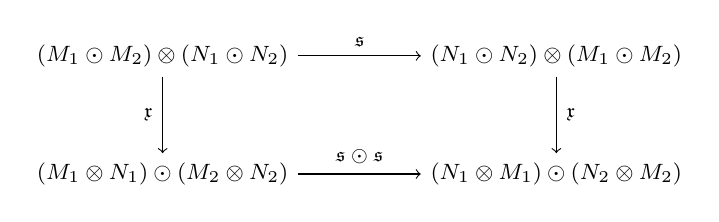
\begin{tikzpicture}
		\node (A) at (0,1.5) {\footnotesize{$(M_1 \odot M_2) \otimes (N_1 \odot N_2)$}};
		\node (A') at (0,0) {\footnotesize{$(M_1\otimes N_1) \odot (M_2\otimes N_2)$}};
		\node (B) at (5,1.5) {\footnotesize{$(N_1\odot N_2) \otimes (M_1 \odot M_2)$}};
		\node (B') at (5,0) {\footnotesize{$(N_1 \otimes M_1) \odot (N_2 \otimes M_2)$}};
		%
		\path[->,font=\scriptsize]
		(A) edge node[left]{$\mathfrak{x}$} (A')
		(A) edge node[above]{$\mathfrak{s}$} (B)
		(B) edge node[right]{$\mathfrak{x}$} (B')
		(A') edge node[above]{$\mathfrak{s} \odot \mathfrak{s}$} (B');
		\end{tikzpicture}
		%
		\quad
		%
		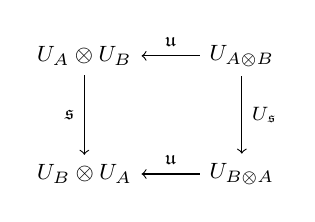
\begin{tikzpicture}
		\node (A) at (0,1.5) {\footnotesize{$U_A \otimes U_B$}};
		\node (A') at (0,0) {\footnotesize{$U_B\otimes U_A$}};
		\node (B) at (2,1.5) {\footnotesize{$U_{A\otimes B} $}};
		\node (B') at (2,0) {\footnotesize{$U_{B\otimes A}$}};
		%
		\path[->,font=\scriptsize]
		(A) edge node[left]{$\mathfrak{s}$} (A')
		(B) edge node[above]{$\mathfrak{u}$} (A)
		(B) edge node[right]{$U_\mathfrak{s}$} (B')
		(B') edge node[above]{$\mathfrak{u}$} (A');
		\end{tikzpicture}
		\]
		\setcounter{mondbl}{\value{enumi}}
	\end{enumerate}
	Finally, a symmetric monoidal double category is braided and
	\begin{enumerate}
		\setcounter{enumi}{\value{mondbl}}
		\item $\dblcat{D}_{0}$ and $\dblcat{D}_{1}$ are in fact symmetric monoidal.
	\end{enumerate}
\end{defn}

%DEFINITION -- Companion and Conjoint
%
\begin{defn}
	\label{def:CompanionConjoint}
	Let $\mathbb{D}$ be a double category and $f \from A\to B$ a vertical $1$-cell.  A \textbf{companion} of $f$ is a horizontal $1$-cell
	$\hat{f} \from A \hto B$ together with $2$-cells
	\[
	\raisebox{-0.5\height}{
		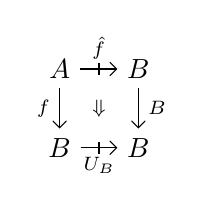
\begin{tikzpicture}
		\node (A) at (0,1) {$A$};
		\node (B) at (1,1) {$B$};
		\node (A') at (0,0) {$B$};
		\node (B') at (1,0) {$B$};
		%
		\path[->,font=\scriptsize,>=angle 90]
		(A) edge node[above]{$\hat{f}$} (B)
		(A) edge node[left]{$f$} (A')
		(B) edge node[right]{$B$} (B')
		(A') edge node[below]{$U_B$} (B');
		%
		\draw (0.5,.925) -- (0.5,1.075);
		\draw (0.5,-.075) -- (0.5,.075);
		\node () at (0.5,0.5) {\scriptsize{$\Downarrow$}};
		\end{tikzpicture}
	}
	%
	\quad \text{and} \quad
	%
	\raisebox{-0.5\height}{
		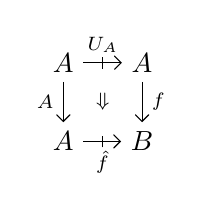
\begin{tikzpicture}
		\node (A) at (0,1) {$A$};
		\node (B) at (1,1) {$A$};
		\node (A') at (0,0) {$A$};
		\node (B') at (1,0) {$B$};
		%
		\path[->,font=\scriptsize,>=angle 90]
		(A) edge node[above]{$U_A$} (B)
		(A) edge node[left]{$A$} (A')
		(B) edge node[right]{$f$} (B')
		(A') edge node[below]{$\hat{f}$} (B');
		%
		\draw (0.5,.925) -- (0.5,1.075);
		\draw (0.5,-.075) -- (0.5,.075);
		\node () at (0.5,0.5) {\scriptsize{$\Downarrow$}};
		\end{tikzpicture}
	}
	\]
	such that the following equations hold:
	\begin{equation}
	\label{eq:CompanionEq}
	\raisebox{-0.5\height}{
		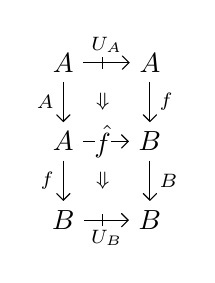
\begin{tikzpicture}
		\node (A) at (0,2) {$A$};
		\node (B) at (1.1,2) {$A$};
		\node (A') at (0,1) {$A$};
		\node (B') at (1.1,1) {$B$};
		\node (A'') at (0,0) {$B$};
		\node (B'') at (1.1,0) {$B$};
		%
		\path[->,font=\scriptsize,>=angle 90]
		(A) edge node[left]{$A$} (A')
		(A') edge node[left]{$f$} (A'')
		(B) edge node[right]{$f$} (B')
		(B') edge node[right]{$B$} (B'')
		(A) edge node[above]{$U_A$} (B)
		(A') edge  (B')
		(A'') edge node[below]{$U_B$} (B'');
		%
		\draw (0.5,1.925) -- (0.5,2.075);
		\draw[line width=2mm,white] (0.5,.925) -- (0.5,1.075);
		\draw (0.5,-.075) -- (0.5,.075);
		\node () at (0.5,0.5) {\scriptsize{$\Downarrow$}};
		\node () at (0.5,1.5) {\scriptsize{$\Downarrow$}};
		\node () at (0.5,1) {$\hat{f}$};
		\end{tikzpicture}
	}
	%
	\raisebox{-0.5\height}{=}
	%
	\raisebox{-0.5\height}{
		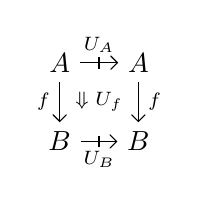
\begin{tikzpicture}
		\node (A) at (0,1) {$A$};
		\node (B) at (1,1) {$A$};
		\node (A') at (0,0) {$B$};
		\node (B') at (1,0) {$B$};
		%
		\path[->,font=\scriptsize,>=angle 90]
		(A) edge node[left]{$f$} (A')
		(B) edge node[right]{$f$} (B')
		(A) edge node[above]{$U_A$} (B)
		(A') edge node[below]{$U_B$} (B');
		%
		\draw (0.5,.925) -- (0.5,1.075);
		\draw (0.5,-.075) -- (0.5,.075);
		\node () at (0.5,0.5) {\scriptsize{$\Downarrow U_f$}};
		\end{tikzpicture}
	}
	%
	\raisebox{-0.5\height}{\text{   and   }}
	%
	\raisebox{-0.5\height}{
		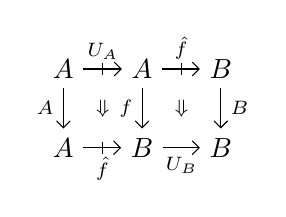
\begin{tikzpicture}
		\node (A) at (0,1) {$A$};
		\node (A') at (0,0) {$A$};
		\node (B) at (1,1) {$A$};
		\node (B') at (1,0) {$B$};
		\node (C) at (2,1) {$B$};
		\node (C') at (2,0) {$B$};
		%
		\path[->,font=\scriptsize,>=angle 90]
		(A) edge node[left]{$A$} (A')
		(B) edge node[left]{$f$} (B')
		(C) edge node[right]{$B$} (C')
		(A) edge node[above]{$U_A$} (B)
		(B) edge node[above]{$\hat{f}$} (C)
		(A') edge node[below]{$\hat{f}$} (B')
		(B') edge node[below]{$U_B$} (C');
		%
		\draw (1.5,0.925) -- (1.5,1.075);
		\draw (1.5,0.925) -- (1.5,1.075);
		\draw (0.5,.925) -- (0.5,1.075);
		\draw (0.5,-.075) -- (0.5,.075);
		\node () at (0.5,0.5) {\scriptsize{$\Downarrow$}};
		\node () at (1.5,0.5) {\scriptsize{$\Downarrow$}};
		\end{tikzpicture}
	}
	%
	\raisebox{-0.5\height}{=}
	%
	\raisebox{-0.5\height}{
		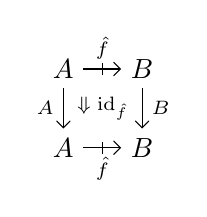
\begin{tikzpicture}
		\node (A) at (0,1) {$A$};
		\node (B) at (1,1) {$B$};
		\node (A') at (0,0) {$A$};
		\node (B') at (1,0) {$B$};
		%
		\path[->,font=\scriptsize,>=angle 90]
		(A) edge node[left]{$A$} (A')
		(B) edge node[right]{$B$} (B')
		(A) edge node[above]{$\hat{f}$} (B)
		(A') edge node[below]{$\hat{f}$} (B');
		%
		\draw (0.5,.925) -- (0.5,1.075);
		\draw (0.5,-.075) -- (0.5,.075);
		\node () at (0.5,0.5) {\scriptsize{$\Downarrow \id_{\hat{f}}$}};
		\end{tikzpicture}
	}
	\end{equation}
	A \textbf{conjoint} of $f$, denoted $\check{f} \from B \hto A$, is a companion of $f$ in the double category $\dblcat{D}^{h\cdot\mathrm{op}}$ obtained by reversing the horizontal 1-cells, but not the vertical $1$-cells, of $\dblcat{D}$.
\end{defn}

\begin{defn}
	\label{def:Fibrant}
	We say that a double category is \emph{fibrant} if every vertical $1$-cell has both a companion and a conjoint. If every invertible vertical $1$-cell has both a companion and a conjoint, then we say the double category is \emph{isofibrant}.
\end{defn}

The next theorem, which plays a crucial role in this paper, was proven by Mike Shulman.  

\begin{thm}[{\cite[Theorem 5.1]{Shul}}]
	\label{thm:DoubleGivesBi}
	Let $\dblcat{D}$ be an isofibrant symmetric monoidal double category. Then $H(\dblcat{D})$ is a symmetric monoidal bicategory.  
\end{thm}


%%%%%%%%%%%%%%%%%%%%%%%%%%%%%%%%%%%%%%%%%%%%%%%%%%%%%%%%%%
\subsection{Duality in bicategories} % DUALITY
\label{sec:CompactClosed}
%%%%%%%%%%%%%%%%%%%%%%%%%%%%%%%%%%%%%%%%%%%%%%%%%%%%%%%%%%

In this section, we suppress the notation for a monoidal operation and instead write $LR$ for the monoidal product of objects $L$ and $R$ and $fg$ for the monoidal product of morphisms $f$ and $g$.  This will reserve the symbol `$\otimes$' for the horizontal composition functor in the definition of a bicategory.

\begin{defn}
	\label{def:DualPairCat}
	A \emph{dual pair} in a monoidal category is a tuple $(L,R,e,c)$ with objects $L$ and $R$, called the left and right duals, and morphisms
	\[
		e \from LR \to I 
		\quad \quad 
		c \from I \to RL,
	\]
	called evaluation and coevaluation such that 
	\[
	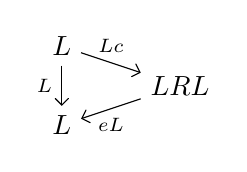
\begin{tikzpicture}
		\node (L1) at (0,1) {$L$};
		\node (L2) at (0,0) {$L$};
		\node (LRL) at (1.5,0.5) {$LRL$};
		%
		\path[->,font=\scriptsize,>=angle 90]
		(L1) edge node[left]{$L$} (L2)
		(L1) edge node[above]{$Lc$} (LRL)
		(LRL) edge node[below]{$eL$} (L2);
	\end{tikzpicture}
	%
	\quad \quad
	%
	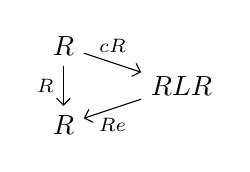
\begin{tikzpicture}
		\node (R1) at (0,1) {$R$};
		\node (R2) at (0,0) {$R$};
		\node (RLR) at (1.5,0.5) {$RLR$};
		%
		\path[->,font=\scriptsize,>=angle 90]
		(R1) edge node[left]{$R$} (R2)
		(R1) edge node[above]{$cR$} (RLR)
		(RLR) edge node[below]{$Re$} (R2);
	\end{tikzpicture}	
	\]
\end{defn}

\begin{defn}
	\label{def:DualPairBicat}
	A \emph{dual pair} in a monoidal bicategory is a tuple $(L,R,e,c,\alpha,\beta)$ with objects $L$ and $R$, $1$-cells
	\[
		e \from LR \to I \quad \quad c \from I \to RL,
	\]
	and invertible $2$-cells $\alpha$, $\beta$
	\[
	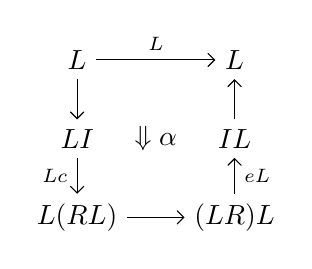
\begin{tikzpicture}
		\node (L1) at (0,2) {$L$};
		\node (LI) at (0,1) {$LI$};
		\node (LRL1) at (0,0) {$L(RL)$};
		\node (LRL2) at (2,0) {$(LR)L$};
		\node (IL) at (2,1) {$IL$};
		\node (L2) at (2,2) {$L$};
		%
		\path[->,font=\scriptsize,>=angle 90]
		(L1) edge (LI)
		(LI) edge node[left] {$Lc$} (LRL1)
		(LRL1) edge (LRL2)
		(LRL2) edge node[right] {$eL$} (IL)
		(IL) edge (L2)
		(L1) edge node[above] {$L$} (L2);
		%
		\node () at (1,1) {$\Downarrow \alpha$};
	\end{tikzpicture}
	%
	\quad \quad
	%
	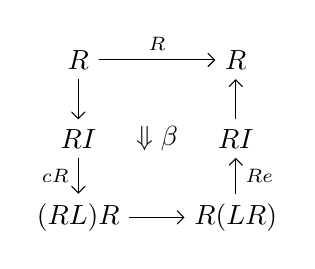
\begin{tikzpicture}
		\node (L1) at (0,2) {$R$};
		\node (LI) at (0,1) {$RI$};
		\node (LRL1) at (0,0) {$(RL)R$};
		\node (LRL2) at (2,0) {$R(LR)$};
		\node (IL) at (2,1) {$RI$};
		\node (L2) at (2,2) {$R$};
		%
		\path[->,font=\scriptsize,>=angle 90]
		(L1) edge (LI)
		(LI) edge node[left] {$cR$} (LRL1)
		(LRL1) edge (LRL2)
		(LRL2) edge node[right] {$Re$} (IL)
		(IL) edge (L2)
		(L1) edge node[above] {$R$} (L2);
		%
		\node () at (1,1) {$\Downarrow \beta$};
	\end{tikzpicture}
	\]
	called cusp isomorphisms.
	
	If this data satisfies the swallowtail equations in the sense that the diagrams in Figure \ref{fig:Swallowtail} are identities, then we call it a \emph{coherent dual pair}.
\end{defn}

\begin{remark}
\label{rem:Swallowtail}
	To prevent cluttering the diagrams in Figure \ref{fig:Swallowtail}, we will only write $a,\rho,\lambda$ for the bicategory structure maps even when we actually mean their inverse.
\end{remark}

\begin{figure}[h]
	%
	%  DIAGRAM 1
	%
	\[
	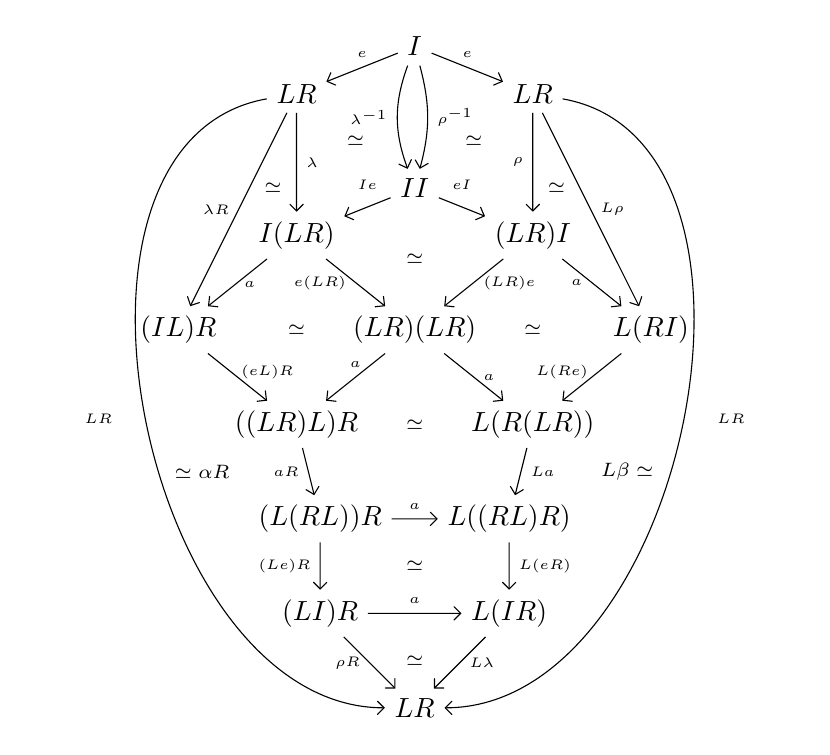
\begin{tikzpicture}[scale=0.60]
	\node (A) at (0,0) {$I$};
	\node (B) at (-2.5,-1) {$L R$};
	\node (C) at (2.5,-1) {$L R$};
	\node (D) at (0,-3) {$I I$};
	\node (E) at (-2.5,-4) {$I (L R)$};
	\node (F) at (2.5,-4) {$(L R) I$};
	\node (G) at (0,-6) {$(L R) (L R)$};
	\node (H) at (-5,-6) {$(I L) R$};
	\node (I) at (5,-6) {$L (R I)$};
	\node (J) at (-2.5,-8) {$((L R) L)  R$};
	\node (K) at (2.5,-8) {$L (R (L R))$};
	\node (L) at (-2,-10) {$(L (R L)) R$};
	\node (M) at (2,-10) {$L  ((R L) R)$};
	\node (N) at (-2,-12) {$(L I) R$};
	\node (O) at (2,-12) {$L (I R)$};
	\node (P) at (0,-14) {$L  R$};
	%
	%  2-CELLS
	%
	\node (Q) at (-1.25,-2) {\scriptsize{$\simeq$}};
	\node (R) at (1.25,-2) {\scriptsize{$\simeq$}};
	\node (S) at (0,-4.5) {\scriptsize{$\simeq$}};
	\node (T) at (-3,-3) {\scriptsize{$\simeq $}};
	\node (U) at (3,-3) {\scriptsize{$\simeq$}};
	\node (V) at (-2.5,-6) {\scriptsize{$\simeq$}};
	\node (W) at (2.5,-6) {\scriptsize{$\simeq$}};
	\node (X) at (0,-8) {\scriptsize{$\simeq$}};
	\node (Y) at (0,-11) {\scriptsize{$\simeq$}};
	\node (Z) at (0,-13) {\scriptsize{$\simeq$}};
	\node (A1) at (-4.5,-9) {\scriptsize{$\simeq \alpha R$}};
	\node (A2) at (4.5,-9) {\scriptsize{$L \beta \simeq$}};
	%
	\path[->,font=\tiny,>=angle 90]
	(A) edge node[above]{$e$} (B)
	(A) edge node[above]{$e$} (C)
	(A) edge[out=-110,in=110] node[left]{$\lambda^{-1}$} (D)
	(A) edge[out=-75,in=75] node[right]{$\rho^{-1}$} (D)
	(B) edge node[right]{$\lambda$}(E)
	(C) edge node[left]{$\rho$} (F)
	(D) edge node[left=0.2cm,above=0.1cm]{$I e$} (E)
	(D) edge node[left=0.2cm,above=0.1cm]{$e I$} (F)
	(E) edge node[below,left,pos=0.5]{$e (L R)$} (G)
	(F) edge node[below,right]{$(L R) e$} (G)
	(B) edge node[above,left]{$\lambda R$} (H)
	(C) edge node[above,right]{$L \rho$} (I)
	(E) edge node[below,right,pos=0.55]{$a$} (H)
	(F) edge node[below,left]{$a$} (I)
	(H) edge node[above,right,pos=0.4]{$(e L) R$} (J)
	(G) edge node[above]{$a$} (J)
	(I) edge node[above,left,pos=0.4]{$L (R e)$} (K)
	(G) edge node[above,right]{$a$} (K)
	(J) edge node[left]{$a R$} (L)
	(K) edge node[right]{$L a$} (M)
	(L) edge node[above]{$a$} (M)
	(L) edge node[left]{$(L  e) R$} (N)
	(M) edge node[right]{$L (e R)$} (O)
	(N) edge node[above]{$a$} (O)
	(N) edge node[below,left]{$\rho R$} (P)
	(O) edge node[below,right]{$L \lambda$} (P)
	(B) edge [out=-170,in=-180] node [below=0.3cm,left=0.3cm] {$L R$} (P)
	(C) edge [in=-360,out=-370,] node [below=0.3cm,right=0.3cm] {$LR$} (P);
	\end{tikzpicture}
	\]
	%
	%  DIAGRAM 2
	%
	\[
	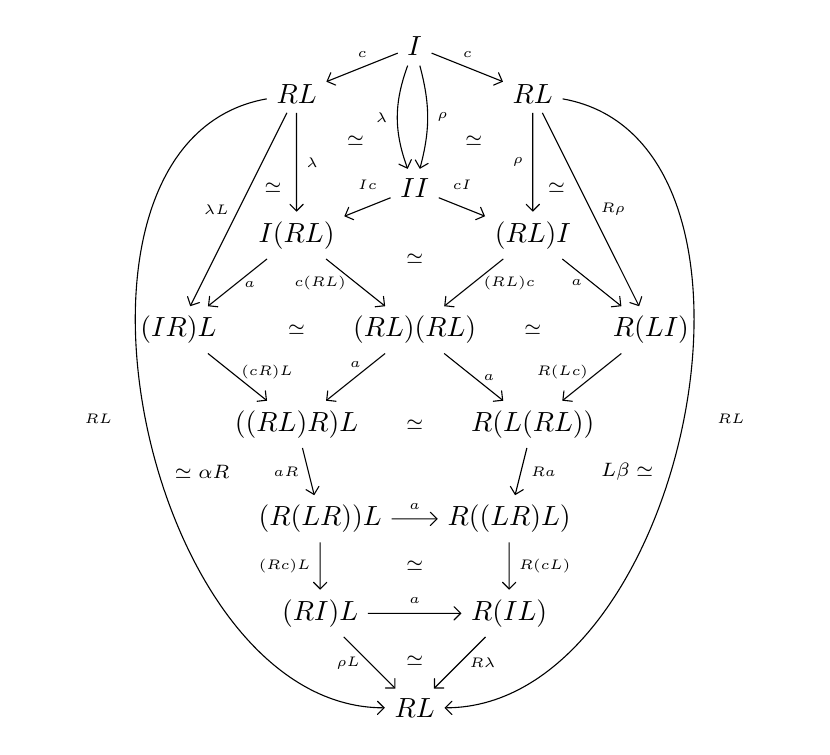
\begin{tikzpicture}[scale=0.60]
	\node (A) at (0,0) {$I$};
	\node (B) at (-2.5,-1) {$RL$};
	\node (C) at (2.5,-1) {$RL$};
	\node (D) at (0,-3) {$I I$};
	\node (E) at (-2.5,-4) {$I (RL)$};
	\node (F) at (2.5,-4) {$(RL) I$};
	\node (G) at (0,-6) {$(RL) (RL)$};
	\node (H) at (-5,-6) {$(I R) L$};
	\node (I) at (5,-6) {$R (L I)$};
	\node (J) at (-2.5,-8) {$((RL) R)  L$};
	\node (K) at (2.5,-8) {$R (L (R L))$};
	\node (L) at (-2,-10) {$(R (L R)) L$};
	\node (M) at (2,-10) {$R  ((L R) L)$};
	\node (N) at (-2,-12) {$(R I) L$};
	\node (O) at (2,-12) {$R (I L)$};
	\node (P) at (0,-14) {$R  L$};
	%
	%  2-CELLS
	%
	\node (Q) at (-1.25,-2) {\scriptsize{$\simeq$}};
	\node (R) at (1.25,-2) {\scriptsize{$\simeq$}};
	\node (S) at (0,-4.5) {\scriptsize{$\simeq$}};
	\node (T) at (-3,-3) {\scriptsize{$\simeq $}};
	\node (U) at (3,-3) {\scriptsize{$\simeq$}};
	\node (V) at (-2.5,-6) {\scriptsize{$\simeq$}};
	\node (W) at (2.5,-6) {\scriptsize{$\simeq$}};
	\node (X) at (0,-8) {\scriptsize{$\simeq$}};
	\node (Y) at (0,-11) {\scriptsize{$\simeq$}};
	\node (Z) at (0,-13) {\scriptsize{$\simeq$}};
	\node (A1) at (-4.5,-9) {\scriptsize{$\simeq \alpha R$}};
	\node (A2) at (4.5,-9) {\scriptsize{$L \beta \simeq$}};
	%
	\path[->,font=\tiny,>=angle 90]
	(A) edge[->] node[above]{$c$} (B)
	(A) edge[->] node[above]{$c$} (C)
	(A) edge[->,out=-110,in=110] node[left]{$\lambda$} (D)
	(A) edge[->,out=-75,in=75] node[right]{$\rho$} (D)
	(B) edge[->] node[right]{$\lambda$}(E)
	(C) edge[->] node[left]{$\rho$} (F)
	(D) edge[->] node[left=0.2cm,above=0.1cm]{$I c$} (E)
	(D) edge[->] node[left=0.2cm,above=0.1cm]{$c I$} (F)
	(E) edge[->] node[below,left,pos=0.5]{$c (R L)$} (G)
	(F) edge[->] node[below,right]{$(R L) c$} (G)
	(B) edge[->] node[above,left]{$\lambda L$} (H)
	(C) edge[->] node[above,right]{$R \rho$} (I)
	(E) edge[->] node[below,right,pos=0.55]{$a$} (H)
	(F) edge[->] node[below,left]{$a$} (I)
	(H) edge[->] node[above,right,pos=0.4]{$(c R) L$} (J)
	(G) edge[->] node[above]{$a$} (J)
	(I) edge[->] node[above,left,pos=0.4]{$R (L c)$} (K)
	(G) edge[->] node[above,right]{$a$} (K)
	(J) edge[->] node[left]{$a R$} (L)
	(K) edge[->] node[right]{$R a$} (M)
	(L) edge[->] node[above]{$a$} (M)
	(L) edge[->] node[left]{$(R  c) L$} (N)
	(M) edge[->] node[right]{$R (c L)$} (O)
	(N) edge[->] node[above]{$a$} (O)
	(N) edge[->] node[below,left]{$\rho L$} (P)
	(O) edge[->] node[below,right]{$R \lambda$} (P)
	(B) edge[->,out=-170,in=-180] node [below=0.3cm,left=0.3cm] {$R L$} (P)
	(C) edge[->,in=-360,out=-370] node [below=0.3cm,right=0.3cm] {$RL$} (P);
	\end{tikzpicture}
	\]
	\caption{The swallowtail diagrams for (co)evaluation}
	\label{fig:Swallowtail}
\end{figure}

Recall that a symmetric monoidal category is called \emph{compact closed} if every object is part of a dual pair. We can generalize this idea to bicategories by introducing $2$-cells and some coherence axioms to ensure the $2$-cells play nicely. The following definition is due to Stay \cite{Stay}.

\begin{defn}
	\label{def:CompClosdBicat}
	A symmetric monoidal bicategory is called \emph{compact closed} if each object $L$ has an associated coherent dual pair. 
\end{defn}

The difference between showing compact closededness in categories versus bicategories is quite large because of the swallowtail equations.  It is no surprise that these can be incredibly tedious to work with.  Fortunately, Pstragowski proved a wonderful strictification theorem in \cite[p.~22]{Piotr} that effectively circumvents the need to consider the swallowtail equations.  

\begin{thm}[{\cite{Piotr}}]
	\label{thm:StrictingDualPairs}
	Given a dual pair $(L,R,e,c,\alpha,\beta)$, we can find a cusp isomorphism $\beta'$ such that $(L,R,e,c,\alpha,\beta')$ is a coherent dual pair.
\end{thm}

There is a striking resemblance between dual pairs as defined above and adjoint pairs. This similarity is worth exploring. Let's recall the unit-counit definition of a pair of adjoint functors.  Given a pair of functors $F \from \cat{A} \to \cat{B}$ and $G \from \cat{B} \to \cat{A}$, we say that they are an adjoint pair if there are natural isomorphisms $\eta \from \id_{A} \to GF$ and $\epsilon \from FG \to \id_B$ such that 
\[
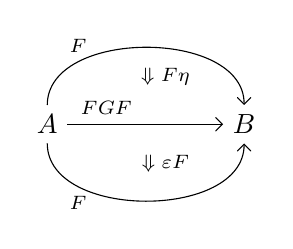
\begin{tikzpicture}
	\node (A) at (0,0) {$A$};
	\node (B) at (2.5,0) {$B$};
	%
	\path[->,font=\scriptsize,>=angle 90]
	(A) edge[out=90,in=90] node[above,pos=.25]{$F$} (B)
		edge node[above,pos=.25]{$FGF$} (B)
		edge[out=-90,in=-90] node[below,pos=.25]{$F$} (B);
	%
	\node () at (1.5,0.6) {\scriptsize{$\Downarrow F \eta$}};
	\node () at (1.5,-0.5) {\scriptsize{$\Downarrow \epsilon F$}};
\end{tikzpicture}
%
\quad \quad 
%
\begin{tikzpicture}
	\node (B) at (0,0) {$B$};
	\node (A) at (2.5,0) {$A$};
	%
	\path[->,font=\scriptsize,>=angle 90]
	(B) edge[out=90,in=90] node[above,pos=.25]{$G$} (A)
		edge node[above,pos=.25]{$GFG$} (A)
		edge[out=-90,in=-90] node[below,pos=.25]{$G$} (A);
	%
	\node () at (1.5,0.6) {\scriptsize{$\Downarrow \eta G$}};
	\node () at (1.5,-0.5) {\scriptsize{$\Downarrow G \epsilon$}};
\end{tikzpicture}
\]
each compose to their respective identity natural isomorphisms. Now, there is no reason for this sort of data to be restricted to only $\cat{Cat}$. Using the intuition from an adjoint pairs in $\cat{Cat}$, we will generalize adjoints to arbitrary bicategories by replacing categories with objects, functors with $1$-cells, and natural transformations with $2$-cells.

\begin{defn}
	There is an \emph{adjunction} between $1$-cells $f \from X \to Y$ and $g \from Y \to X$ in a bicategory if there are $2$-cells $\eta \from 1_{X} \to gf$ and $\epsilon \from fg \to 1_Y$ such that the compositions
	\[
	\begin{tikzpicture}
		\node (X) at (0,0) {$X$};
		\node (Y) at (2.5,0) {$Y$};
		%
		\path[->,font=\scriptsize,>=angle 90]
		(X) edge[out=90,in=90] node[above,pos=.25]{$f$} (Y)
			edge node[above,pos=.25]{$fgf$} (Y)
			edge[out=-90,in=-90] node[below,pos=.25]{$f$} (Y);
		%
		\node () at (1.5,0.7) {\scriptsize{$\Downarrow f \otimes \eta$}};
		\node () at (1.5,-0.5) {\scriptsize{$\Downarrow \epsilon \otimes  f$}};
	\end{tikzpicture}
	%
	\quad \quad 
	%
	\begin{tikzpicture}
		\node (B) at (0,0) {$Y$};
		\node (A) at (2.5,0) {$X$};
		%
		\path[->,font=\scriptsize,>=angle 90]
		(B) edge[out=90,in=90] node[above,pos=.25]{$g$} (A)
			edge node[above,pos=.25]{$gfg$} (A)
			edge[out=-90,in=-90] node[below,pos=.25]{$g$} (A);
		%
		\node () at (1.5,0.7) {\scriptsize{$\Downarrow \eta \otimes g$}};
		\node () at (1.5,-0.5) {\scriptsize{$\Downarrow g \otimes \epsilon$}};
	\end{tikzpicture}
	\]
	each coincide with identity $2$-cells. Here, we say that $f$ is a left adjoint, $g$ is a right adjoint and write $f \dashv g$.  We also call $\eta$ the unit and $\epsilon$ the counit of the adjuntion. 
	
	An \emph{equivalence} between objects $X,Y$ of a bicategory consists of a pair of $1$-cells $f \from X \to Y$ and $g \from Y \to X$ and invertible $2$-cells $\eta \from fg \to \id_Y$ and $\epsilon \from \id_X \to gf$.  In case $\eta$ and $\epsilon$ are the unit of counit of an adjunction $f \dashv g$, we say there is an \emph{adjoint equivalence}.
\end{defn}

The thing to do now is to recast the definitions of duality in terms of adjunctions.  The benefit of this is that it allows us to define a stronger condition than duals.

Recall that a monoidal category $\cat{M}$ can be thought of as a bicategory $\mathcal{B}\cat{M}$ with a single object, $\cat{M}$-objects as $1$-cells, and the $\cat{M}$-morphisms as the $2$-cells.  The composition functor of $\mathcal{B} \cat{M}$ is given by the monoidal structure of $\cat{M}$. Then, an $\cat{M}$-object $L$ has a right dual $R$ if and only if $L \dashv R$ in $\mathcal{B} \cat{M}$. 

Given a bicategory $\cat{B}$, define its homotopy category $\op{ho} \cat{B}$ by keeping the same objects and let the morphisms be isomorphism classes of $1$-cells. Now, suppose that $\cat{B}$ has a monoidal structure. The category $\op{ho} \cat{B}$ inherits this structure and so we can consider the bicategory $\mathcal{B} (\op{ho} \cat{B})$. This allows us to define duals in $\op{ho}\cat{B}$ via adjoints as above. A $\cat{B}$-object $L$ has a right dual if the $(\op{ho} \cat{B})$-object $L$ has a right dual.

Having seen dual pairs defined in terms of adjoints, we can go on to define an even stronger condition called fully dual.  We will take a simplified approach and only say enough for our needs. For a more fundamental and general account of full dualizability see \cite{Lurie,Piotr}. 

To prepare for the definition fully dual pairs, we construct the following universal bicategory. Let $\cat{S}$ be a symmetric monoidal bicategory. There exists another symmetric monoidal bicategory $\cat{S}^{\text{fd}}$ with duals and a symmetric monoidal functor $i \from \cat{S}^{\text{fd}} \to \cat{S}$.  The idea behind the construction of $\cat{S}^{\text{fd}}$ is iterating a process of removing morphisms from $\cat{S}$ that do not have both a left or right adjoint. Then $\cat{S}^{\text{fd}}$ has the universal property where, given any other symmetric monoidal bicategory $\cat{S}'$ with duals and a symmetric monoidal functor $F \from \cat{S}' \to \cat{S}$, then $F$ factors uniquely up to isomorphism through $i$. Another way to think about $\cat{S}^{\text{fd}}$ is that it is the maximal sub-bicategory of $\cat{S}$ with respect to the property that every $1$-cell has left and right adjoints.  

\begin{defn}
\label{def:FullDual}
	An object in a symmetric monoidal bicategory $\cat{S}$ is fully dualizable if it is in the essential image of $i \from \cat{S}^{\text{fd}} \to \cat{S}$
\end{defn}  

On the surface, it seems a bit dire to check whether an object is fully dualizable, but there is a nice characterization of this property that makes checking for it a bit easier.

\begin{thm}[{\cite[Prop.~4.2.3]{Lurie}}]
	An object in a bicategory is fully dualizable if it admits a dual and the evaluation map admits a left and right adjoint.  
\end{thm}

Suppose that we have an dual pair $(L,R,e,c,\alpha,\beta)$ in a bicategory and left adjoints $e^\text{L} \dashv e$ and $c^\text{L} \dashv c$.  There is a 1-cell $q$, called the \emph{Serre automorphism} of $L$, and its weak inverse $q^{-1}$ defined to be the respective composites
\begin{align*}
	L \to LI 
	\xto{Lc} LRL 
	\xto{\sigma L} RLL 
	\xto{c^\text{L}L} IL
	\to L \\
	L \to LI
	\xto{Le^\text{L}} LLR
	\xto{L\sigma} LRL
	\xto{eL} IL
	\to L.
\end{align*}
See Remark 4.2.4 in \cite{Lurie} to see the story of why $q$ is named the Serre automorphism.  

\begin{defn}
	A fully dual pair $(L,R,e,c,\alpha,\beta)$ is \emph{coherent} if it is coherent as a dual pair, there are left adjoints $e^{\text{L}}$ and $c^{\text{L}}$ so that the Serre automorphism pair $q,q^{-1}$ is an adjoint equivalence, and the composites diagrammed in Figures \ref{fig:CuspCounitsCompositeI} and \ref{fig:CuspCounitsCompositeII} are equal.  
\end{defn}

\todo{Piotr says the eggs are a framed analog of cusp flip relations from the presentation of the oriented bordism bicat from Chris SP in his CLASSIFICATION TQFTs paper}

\begin{figure}
\[
\begin{tikzpicture}
	%
	%  0-CELLS
	%
	\node (1) at (1,-2) {\scriptsize{$L$}};
	\node (2) at (0,-1) {\scriptsize{$LI$}};
	\node (3) at (0,0) {\scriptsize{$L(RL)$}};
	\node (4) at (0,1) {\scriptsize{$(LR)L$}};
	\node (5) at (0,2) {\scriptsize{$IL$}};
	\node (6) at (1,3) {\scriptsize{$(RL)L$}};
	\node (7) at (4,3) {\scriptsize{$(RL)L$}};
	\node (8) at (7,3) {\scriptsize{$(LR)L$}};
	\node (9) at (8,2) {\scriptsize{$L(RL)$}};
	\node (10) at (8,1) {\scriptsize{$L(LR)$}};
	\node (11) at (8,0) {\scriptsize{$L(LR)$}};
	\node (12) at (8,-1) {\scriptsize{$LI$}};
	\node (13) at (7,-2) {\scriptsize{$L$}};
	%
	%  1-CELLS
	%
	\path[->,font=\tiny]
	(1) edge node[left,below]{$\rho$} (2)
	(2) edge node[left]{$Lc$} (3)
	(3) edge node[left]{$a$} (4)
	(4) edge node[left]{$eL$} (5)
	(5) edge node[above,left]{$cL$} (6)
	(6) edge node[above]{$(Rq^{-1})L$} (7)
	(7) edge node[above]{$\sigma L$} (8)
	(8) edge node[above]{$a$} (9)
	(9) edge node[right]{$L \sigma$} (10)
	(10) edge node[right]{$L(qR)$} (11)
	(11) edge node[right]{$Le$} (12)
	(12) edge node[right]{$\rho$} (13)
	(1) edge node[above]{$L$} (13)
	%
	(2) edge node[below]{$(LR)L$} (12)
	(3) edge[out=0,in=225] node[below]{$L(RL)$} (9)
	(4) edge[out=0,in=225] node[below]{$LI$} (8);
	%
	%  2-CELLS
	%
	\node () at (2,2) {\scriptsize{$\Downarrow \epsilon_L \otimes L $}};
	\node () at (2,0.6) {\scriptsize{$\Downarrow a$}};
	\node () at (2,0-0.5) {\scriptsize{$\Downarrow L \otimes \epsilon_L$}};
	\node () at (2,-1.5) {\scriptsize{$\Downarrow \rho$}};
\end{tikzpicture}
\]
\caption{Cusp-Counits Composite I}
\label{fig:CuspCounitsCompositeI}
\end{figure}

\begin{figure}
\[
\begin{tikzpicture}
	%
	%  0-CELLS BOUNDARY
	%
	\node (1) at (1,-2.5) {\scriptsize{$L$}};
	\node (2) at (0,-1) {\scriptsize{$LI$}};
	\node (3) at (0,0) {\scriptsize{$L(RL)$}};
	\node (4) at (0,1) {\scriptsize{$(LR)L$}};
	\node (5) at (0,2) {\scriptsize{$IL$}};
	\node (6) at (1,3) {\scriptsize{$(RL)L$}};
	\node (7) at (5,3) {\scriptsize{$(RL)L$}};
	\node (8) at (7,3) {\scriptsize{$(LR)L$}};
	\node (9) at (8,2) {\scriptsize{$L(RL)$}};
	\node (10) at (8,1) {\scriptsize{$L(LR)$}};
	\node (11) at (8,0) {\scriptsize{$L(LR)$}};
	\node (12) at (8,-1) {\scriptsize{$LI$}};
	\node (13) at (7,-2.5) {\scriptsize{$L$}};
	%
	%  1-CELLS BOUNDARY
	%
	\path[->,font=\tiny]
	(1) edge node[left,below]{$\rho$} (2)
	(2) edge node[left]{$Lc$} (3)
	(3) edge node[left]{$a$} (4)
	(4) edge node[left]{$eL$} (5)
	(5) edge node[above,left]{$cL$} (6)
	(6) edge node[above]{$(Rq^{-1})L$} (7)
	(7) edge node[above]{$\sigma L$} (8)
	(8) edge node[above]{$a$} (9)
	(9) edge node[right]{$L \sigma$} (10)
	(10) edge node[right]{$L(qR)$} (11)
	(11) edge node[right]{$Le$} (12)
	(12) edge node[right]{$\rho$} (13)
	(1) edge node[above]{$L$} (13);
	%
	%  0-CELLS INTERIOR
	%
	\node (a) at (1,1) {\scriptsize{$L$}};
	\node (b) at (2,2) {\scriptsize{$LI$}};
	\node (b1) at (2,-1.75) {\scriptsize{$L$}};
	\node (c) at (2,1) {\scriptsize{$LI$}};
	\node (d) at (3.5,2) {\scriptsize{$L(RL)$}};
	\node (e) at (3.5,1) {\scriptsize{$L(RL)$}};
	\node (f) at (5.5,2) {\scriptsize{$L(RL)$}};
	\node (g) at (5.5,1) {\scriptsize{$(LR)L$}};
	\node (h) at (3.5,0) {\scriptsize{$(LR)L$}};
	\node (i) at (5.5,0) {\scriptsize{$(LR)L$}};
	\node (j) at (5.5,-1) {\scriptsize{$IL$}};
	\node (k) at (6.75,-1) {\scriptsize{$IL$}};
	\node (l) at (5.5,-1.75) {\scriptsize{$L$}};
	%
	%  1-CELLS INTERIOR
	%
	\path[->,font=\tiny]
	(5) edge node[above]{$\lambda$} (a)
	(1) edge node[right,pos=0.25]{$L$} (a)
	(a) edge node[below,right]{$\rho$} (b)
	(a) edge node[right]{$q$} (b1)
	(1) edge node[below]{$q$} (b1)
	(5) edge node[above]{$\sigma$} (b)
	(b) edge node[right]{$qI$} (c)
	(b1) edge node[right]{$\rho$} (c)
	(b) edge node[above]{$Lc$} (d)
	(c) edge node[below]{$Lc$} (e)
	(d) edge node[right]{$q(LR)$} (e)
	(d) edge node[above]{$L(Rq^{-1})$} (f)
	(7) edge node[right]{$\sigma$} (f)
	(f) edge node[right]{$a$} (g)
	(g) edge node[above,left]{$\sigma$} (9)
	(e) edge node[right]{$a$} (h)
	(g) edge node[right]{$(qR)L$} (i)
	(h) edge node[below]{$(LR)q$} (i)
	(i) edge node[left]{$eL$} (j)
	(j) edge node[above]{$Iq^{-1}$} (k)
	(k) edge node[above]{$\sigma$} (12)
	(k) edge node[left]{$\lambda$} (13)
	(b1) edge node[above]{$L$} (l)
	(j) edge node[left]{$\lambda$} (l)
	(l) edge node[above]{$q^{-1}$} (13);
	%
	%
	%  2-CELLS
	%
	\node () at (0.5,-0.5) {\scriptsize{$\simeq a$}};
	\node () at (1.35,-1) {\scriptsize{$\simeq$}};
	\node () at (1,1.6) {\scriptsize{$\simeq$}};
	\node () at (1.6,0.5) {\scriptsize{$\simeq$}};
	\node () at (2.75,1.5) {\scriptsize{$\simeq$}};
	\node () at (2.75,2.5) {\scriptsize{$\simeq \beta$}};
	\node () at (6.5,2.25) {\scriptsize{$\simeq$}};
	\node () at (4.5,1) {\scriptsize{$\simeq$}};
	\node () at (3.5,-0.75) {\scriptsize{$\simeq \alpha$}};
	\node () at (3,-2) {\scriptsize{$\simeq$}};
	\node () at (6.25,-1.5) {\scriptsize{$\simeq$}};
	\node () at (7.25,-1.5) {\scriptsize{$\simeq$}};
	\node () at (7,0.5) {\scriptsize{$\simeq \beta$}};
\end{tikzpicture}
\]
\caption{Cusp-Counits Composite II}
\label{fig:CuspCounitsCompositeII}
\end{figure}

\begin{thm}[{\cite[Thm.~3.16]{Piotr}}]
	Any fully dualizable object can be completed to a coherent fully dual pair.
\end{thm}
 

%%%%%%%%%%%%%%%%%%%%%%%%%%%%%%%%%%%%%%%%%%%%%%%%%%%%%%%%%%
%%%%%%%%%%%%%%%%%%%%%%%%%%%%%%%%%%%%%%%%%%%%%%%%%%%%%%%%%%
\section{(Co)spans and maps of (co)spans} % SPANS AND MAPS OF SPANS
\label{sec:SpansMaps}
%%%%%%%%%%%%%%%%%%%%%%%%%%%%%%%%%%%%%%%%%%%%%%%%%%%%%%%%%%
%%%%%%%%%%%%%%%%%%%%%%%%%%%%%%%%%%%%%%%%%%%%%%%%%%%%%%%%%%

%%%%%%%%%%%%%%%%%%%%%%%%%%%%%%%%%%%%%%%%%%%%%%%%%%%%%%%%%%
\subsection{Symmetric monoidal bicategories} % SM BICATS
\label{subsec.SpansMapsAreSMBicat}
%%%%%%%%%%%%%%%%%%%%%%%%%%%%%%%%%%%%%%%%%%%%%%%%%%%%%%%%%%

In this section, we show that the bicategory $\bispmap{C}$ of $\cat{C}$-objects, $\cat{C}$-spans, and $\cat{C}$-maps of spans is symmetric monoidal. We also show that the the bicategory $\bicspmap{D}$ of $\cat{D}$-objects, $\cat{D}$-cospans, and $\cat{D}$-maps of cospans is a symmetric monoidal bicategory.  

To this end, we define double categories $\dblspmap{C}$ and $\dblcspmap{D}$.   The objects of $\dblspmap{C}$ are the $\cat{C}$-objects, vertical $1$-cells are the $\cat{C}$-morphisms, horizontal $1$-cells are $\cat{C}$-spans, and $2$-cells are $\cat{C}$-morphisms between the apexes causing the evident diagram to commute (see Figure \ref{fig:2cells}).  The double category $\dblcspmap{D}$ has $\cat{D}$-objects, $\cat{D}$-morphisms for vertical $1$-cells, $\cat{D}$-cospans as horizontal $1$-cells, and $\cat{D}$-maps between apexes of cospans as $2$-cells.  This double category was discussed by Courser in \cite{Cour} and studied in \cite{DawsonParePronk}.

% SYMMETRIC MONOIDAL DOUBLE CATEGORIES
\begin{lem}[{\cite[Prop.~4.2]{Cour}}]
\label{lem:SpanMapsDoubleCat}
	The double categories $\dblspmap{C}$ and $\dblcspmap{D}$ are symmetric monoidal.  
\end{lem}

% ISOFIBRANT
\begin{lem}
	\label{lem:SpanMapsIsofibrant}
	The symmetric monoidal double categories $\dblspmap{C}$ and $\dblcspmap{D}$ are isofibrant.  
\end{lem}

\begin{proof}
	Let $f \from a \to b$ be a vertical $1$-cell in $\dblcspmap{D}$.  The companion $\hat{f}$ is the cospan 
	\[
		a \xto{f} b \gets b
	\]
	with the $2$-cells $\id_b$ and $f$.  The conjoint $\check{f}$ of $f$ is the cospan
	\[
	b \to b \xleftarrow{f} a
	\]
	equipped with the same $2$-cells. 
\end{proof}

Using these Lemmas, we can use results from Shulman to obtain the main theorem of this section.

% SYMMETRIC MONOIDAL BICATEGORIES
\begin{thm}
\label{thm:SpansMapsAreSMBicat}
	The bicategories $\bispmap{C}$ and $\bicspmap{D}$ are symmetric monoidal.
\end{thm}

\begin{proof}
	Apply Theorem \ref{thm:DoubleGivesBi}.
\end{proof}


%%%%%%%%%%%%%%%%%%%%%%%%%%%%%%%%%%%%%%%%%%%%%%%%%%%%%%%%%%
\subsection{Compact closed} % COMPACT CLOSED BICATES
\label{subsec.SpansMapsAreCCBicats}
%%%%%%%%%%%%%%%%%%%%%%%%%%%%%%%%%%%%%%%%%%%%%%%%%%%%%%%%%%

We continue in this section to study duality structure present on the bicategories $\bispmap{C}$ and $\bicspmap{D}$.  

\begin{lem}
\label{lem:PushoutDiagram}
	The diagram
	\[
		\begin{tikzpicture}
			\node (UL) at (0,1) {$X+X+X$};
			\node (LL) at (0,0) {$X+X$};
			\node (UR) at (3,1) {$X+X$};
			\node (LR) at (3,0) {$X$};
			%
			\path[->,font=\scriptsize,>=angle 90]
			(UL) edge node[above] {$X+\nabla$} (UR)
			(UL) edge node[left] {$\nabla +X$} (LL)
			(UR) edge node[right] {$\nabla$} (LR)
			(LL) edge node[above] {$\nabla$} (LR);
		\end{tikzpicture}
	\]
	is a pushout square.
\end{lem}

\begin{proof}
	Suppose we have maps $f,g \from X+X \to Y$ that form a cocone over the span inside the above diagram. Let $\iota \from X \to X+X+X$ include $X$ into the middle copy of $X$. Observe that $\ell \coloneqq (\nabla + X) \circ \iota$ and $r \coloneqq (X + \nabla) \circ \iota$ are, respectively, the left and right inclusions $X \to X+X$. Then $f \circ \ell = g \circ r$ is a map $X \to Y$, which we claim is the unique map making the required diagram commute. Indeed, given $h \from X \to Y$ such that $f = h \circ \nabla = g$.  Then $g \circ r = f \circ \ell = h \circ \nabla \circ \ell = h$.
\end{proof}

\begin{thm}
	\label{thm:SpansMapsAreCCBicat}
	The bicategories $\bispmap{C}$ and $\bicspmap{D}$ are compact closed.
\end{thm}

\begin{proof}
	We will prove this for $\bicspmap{D}$ and use duality to obtain the result for $\bispmap{C}$. To begin, we will show that objects are self dual. Take an object $X$.  Define the evaluation $1$-cell $e \from X + X \tocospan 0$ and coevaluation $1$-cell $c \from 0 \tocospan X+X$ as follows:
	\[
		e = (X+X \xto{\nabla} X \gets 0), \quad \quad 
		c = (0 \to X \xleftarrow{\nabla} X+X).
	\]
	Next we define the cusp isomorphisms, $\alpha$ and $\beta$.
	Note that $\alpha$ is a $2$-cell whose domain is the composite $1$-cell
	\[
		X \xto{\ell}
		X+X \xleftarrow{X+\nabla}
		X+X+X \xto{\nabla +X}
		X+X \xleftarrow{r}
		X
	\]
	and codomain is the identity cospan on $X$.  Use Lemma \ref{lem:PushoutDiagram} and the fact that $\nabla+X = \ell \circ \nabla$ and $X + \nabla = r \circ \nabla$ to see that the composite is the identity cospan on $X$.  The codomain of $\beta$ is also the identity cospan on $X$, which is obtained as the composite $1$-cell
	\[
		X \xto{r}
		X+X \xleftarrow{\nabla+X}
		X+X+X \xto{X+\nabla}
		X+X \xleftarrow{\ell}
		X
	\]
	Take $\alpha$ and $\beta$, each, to be the identity $2$-cell on $X$. Thus we have a dual pair $(X,X,e,c,\alpha,\beta)$. By Theorem \ref{thm:StrictingDualPairs}, we know there is a cusp isomorphism $\beta'$ such that $(X,X,e,c,\alpha,\beta')$ is a coherent dual pair.  
\end{proof}

\todo{Obstacles to fully dualizable}


%%%%%%%%%%%%%%%%%%%%%%%%%%%%%%%%%%%%%%%%%%%%%%%%%%%%%%%%%%
%%%%%%%%%%%%%%%%%%%%%%%%%%%%%%%%%%%%%%%%%%%%%%%%%%%%%%%%%%
% SPANS AND SPANS OF SPANS + OP
\section{(Co)spans and (co)spans of (co)spans}                  
\label{sec:SpansSpans}
%%%%%%%%%%%%%%%%%%%%%%%%%%%%%%%%%%%%%%%%%%%%%%%%%%%%%%%%%%
%%%%%%%%%%%%%%%%%%%%%%%%%%%%%%%%%%%%%%%%%%%%%%%%%%%%%%%%%%

%%%%%%%%%%%%%%%%%%%%%%%%%%%%%%%%%%%%%%%%%%%%%%%%%%%%%%%%%%
\subsection{Symmetric monoidal bicategories} % SM BICATS
\label{subsec.SpansSpanssAreSMBicat}
%%%%%%%%%%%%%%%%%%%%%%%%%%%%%%%%%%%%%%%%%%%%%%%%%%%%%%%%%%

In this section, we will show that bicategories $\bispsp{C}$ and $\bicspcsp{D}$ are symmetric monoidal. Again, we will only prove this for $\bicspcsp{D}$ and note that an analogous argument will show that the same holds for $\bispsp{C}$.  

\begin{defn}
\label{def:DblCatSpanSpan}
	Define a double category $\dblspsp{C}$ whose objects are the $\cat{C}$-objects, vertical $1$-cells are given by isomorphism classes of $\cat{C}$-spans, horizontal $1$-cells are given by $\cat{C}$-spans, and $2$-cells are spans of spans in $\cat{C}$ making the evident diagram commute (see Figure \ref{fig:2cells}). Define the double category $\dblcspcsp{D}$ by replacing $\cat{C}$ with $\cat{D}$ and spans with cospans.  
\end{defn}

% DOUBLE CATEGORIES
\begin{lem}
	\label{lem:SpanSpanDoubleCat}
	Both $\dblspsp{C}$ and $\dblcspcsp{D}$ are actually double categories.  
\end{lem}

\begin{proof}
	We will prove this for the case of $\dblcspcsp{D}$. To simplify notation, we will denote $\dblcspcsp{D}$ by $\dblcat{D}$.
	
	The object category $\dblcat{D}_0$ is the usual category $\cat{Csp(D)}$ of isomorphism classes of cospans in $D$.  The arrow category $\dblcat{D}_1$ has as objects, $\cat{D}$-cospans and as morphisms, isomorphism classes of cospans of cospans. A morphism from $b \from a \tocospan c$ to $b'' \from a'' \tocospan c''$ is given by a diagram
	\begin{equation}
	\label{diag:CspCsp2Cell}
	\raisebox{-0.5\height}{
	\begin{tikzpicture}
		\node (A) at (0,2) {$a$};
		\node (A') at (0,1) {$a'$};
		\node (A'') at (0,0) {$a''$};
		\node (B) at (1,2) {$b$};
		\node (B') at (1,1) {$b'$};
		\node (B'') at (1,0) {$b''$};
		\node (C) at (2,2) {$c$};
		\node (C') at (2,1) {$c'$};
		\node (C'') at (2,0) {$c''$};
		%
		\path[->,font=\scriptsize,>=angle 90]
		% horizontal arrows
		(A) edge node[above]{$$} (B)
		(A') edge node[above]{$$} (B')
		(A'') edge node[above]{$$} (B'')
		(C) edge node[above]{$$} (B)
		(C') edge node[above]{$$} (B')
		(C'') edge node[above]{$$} (B'')
		% vertical arrows
		(A) edge node[left]{$$} (A')
		(A'') edge node[left]{$$} (A')
		(B) edge node[left]{$$} (B')
		(B'') edge node[left]{$$} (B')
		(C) edge node[left]{$$} (C')
		(C'') edge node[left]{$$} (C');	
	\end{tikzpicture}
	}
	\end{equation}
	It is straightforward enough to check that $\dblcat{D}_1$ is a category.
	
	The unit functor $U \from \dblcat{D}_0 \to \dblcat{D}_1$ maps a $\dblcat{D}$-object to the identity cospan on it and a morphism, $b \from a \tocospan c$ to the square 
	\[
	\begin{tikzpicture}
		\node (A) at (0,2) {$a$};
		\node (A') at (0,1) {$a$};
		\node (A'') at (0,0) {$a$};
		\node (B) at (1,2) {$b$};
		\node (B') at (1,1) {$b$};
		\node (B'') at (1,0) {$b$};
		\node (C) at (2,2) {$c$};
		\node (C') at (2,1) {$c$};
		\node (C'') at (2,0) {$c$};
		%
		\path[->,font=\scriptsize,>=angle 90]
		% horizontal arrows
		(A) edge node[above]{$ $} (B)
		(A') edge node[above]{$ $} (B')
		(A'') edge node[above]{$ $} (B'')
		(C) edge node[above]{$ $} (B)
		(C') edge node[above]{$ $} (B')
		(C'') edge node[above]{$ $} (B'')
		% vertical arrows
		(A) edge node[left]{$a$} (A')
		(A'') edge node[left]{$a$} (A')
		(B) edge node[left]{$b$} (B')
		(B'') edge node[left]{$b$} (B')
		(C) edge node[left]{$c$} (C')
		(C'') edge node[left]{$c$} (C');	
	\end{tikzpicture}
	\]
	%
	The source functor $S \from \dblcat{D}_1 \to \dblcat{D}_0$ sends an object $b \from a \tocospan c$ to $a$ and a morphism, say \eqref{diag:CspCsp2Cell}, to $b \from a \tocospan c$.  
	%
	The target functor $T$ is defined similarly. These structure functors satisfy the required equations.  
	
	We can illustrate the action of the composition functor $ \odot \from \dblcat{D}_1 \times_{\dblcat{D}_0} \dblcat{D}_1 \to \dblcat{D}_1$ diagramatically as
	\[
	\raisebox{-0.5\height}{
	\begin{tikzpicture}
		\node (A) at (0,2) {$a$};
		\node (A') at (0,1) {$a'$};
		\node (A'') at (0,0) {$a''$};
		\node (B) at (1,2) {$b$};
		\node (B') at (1,1) {$b'$};
		\node (B'') at (1,0) {$b''$};
		\node (C) at (2,2) {$c$};
		\node (C') at (2,1) {$c'$};
		\node (C'') at (2,0) {$c''$};
		\node (D) at (3,2) {$d$};
		\node (D') at (3,1) {$d'$};
		\node (D'') at (3,0) {$d''$};
		\node (E) at (4,2) {$e$};
		\node (E') at (4,1) {$e'$};
		\node (E'') at (4,0) {$e''$};
		%
		\path[->,font=\scriptsize,>=angle 90]
		% horizontal arrows
		(A) edge node[above]{$$} (B)
		(A') edge node[above]{$$} (B')
		(A'') edge node[above]{$$} (B'')
		(C) edge node[above]{$$} (B)
		(C') edge node[above]{$$} (B')
		(C'') edge node[above]{$$} (B'')
		(C) edge node[above]{$$} (D)
		(C') edge node[above]{$$} (D')
		(C'') edge node[above]{$$} (D'')
		(E) edge node[above]{$$} (D)
		(E') edge node[above]{$$} (D')
		(E'') edge node[above]{$$} (D'')
		% vertical arrows
		(A) edge node[left]{$$} (A')
		(A'') edge node[left]{$$} (A')
		(B) edge node[left]{$$} (B')
		(B'') edge node[left]{$$} (B')
		(C) edge node[left]{$$} (C')
		(C'') edge node[left]{$$} (C')	
		(D) edge node[left]{$$} (D')
		(D'') edge node[left]{$$} (D')
		(E) edge node[left]{$$} (E')
		(E'') edge node[left]{$$} (E');
	\end{tikzpicture}
	}
	\quad
	\xmapsto[]{\odot}
	\quad
	\raisebox{-0.5\height}{
	\begin{tikzpicture}
		\node (A) at (0,2) {$a$};
		\node (A') at (0,1) {$a'$};
		\node (A'') at (0,0) {$a''$};
		\node (B) at (1.5,2) {$b+_{c}d$};
		\node (B') at (1.5,1) {$b'+_{c'}d'$};
		\node (B'') at (1.5,0) {$b''+_{c''}d''$};
		\node (C) at (3,2) {$e$};
		\node (C') at (3,1) {$e'$};
		\node (C'') at (3,0) {$e''$};
		%
		\path[->,font=\scriptsize,>=angle 90]
		% horizontal arrows
		(A) edge node[above]{$$} (B)
		(A') edge node[above]{$$} (B')
		(A'') edge node[above]{$$} (B'')
		(C) edge node[above]{$$} (B)
		(C') edge node[above]{$$} (B')
		(C'') edge node[above]{$$} (B'')
		% vertical arrows
		(A) edge node[left]{$$} (A')
		(A'') edge node[left]{$$} (A')
		(B) edge node[left]{$$} (B')
		(B'') edge node[left]{$$} (B')
		(C) edge node[left]{$$} (C')
		(C'') edge node[left]{$$} (C');	
	\end{tikzpicture}
	}
	\]
	However, showing that $\odot$ preserves composition, which is known as the interchange law, is not trivial so we will prove this as its own lemma immediately following.
	
	The coherence maps $\alpha$, $\lambda$, and $\rho$ all arise from the universal properties of pushouts. Also, each coherence map is sent to an identity map via functors $S$ and $T$. The pentagon and triangle coherence axioms follow from the universal properties of the colimits involved (see \cite{Cour} for more detail).
\end{proof}

% INTERCHANGE LAW
\begin{lem}
	The assignment $\odot$ from Lemma \ref{lem:SpanSpanDoubleCat} preserves composition. In particular, $\odot$ is a functor.
\end{lem}

\begin{proof}
	Let $\alpha, \alpha^\prime, \beta, \beta^\prime$ be composable 2-morphisms given by
	\[
	\begin{tikzpicture}
		\node () at (-0.75,1) {$\alpha =$};
		% nodes
		\node (A) at (0,2) {$a$};
		\node (A') at (0,1) {$a'$};
		\node (A'') at (0,0) {$\ell$};
		\node (B) at (1,2) {$b$};
		\node (B') at (1,1) {$b'$};
		\node (B'') at (1,0) {$m$};
		\node (C) at (2,2) {$c$};
		\node (C') at (2,1) {$c'$};
		\node (C'') at (2,0) {$n$};
		%
		\path[->,font=\scriptsize,>=angle 90]
		% horizontal arrows
		(A) edge node[above]{$$} (B)
		(A') edge node[above]{$$} (B')
		(A'') edge node[above]{$$} (B'')
		(C) edge node[above]{$$} (B)
		(C') edge node[above]{$$} (B')
		(C'') edge node[above]{$$} (B'')
		% vertical arrows
		(A) edge node[left]{$$} (A')
		(A'') edge node[left]{$$} (A')
		(B) edge node[left]{$$} (B')
		(B'') edge node[left]{$$} (B')
		(C) edge node[left]{$$} (C')
		(C'') edge node[left]{$$} (C');	
	\end{tikzpicture}
	%
	\quad \quad
	%
	\begin{tikzpicture}
		\node () at (-0.75,1) {$\alpha' =$};
		% nodes
		\node (A) at (0,2) {$c$};
		\node (A') at (0,1) {$c'$};
		\node (A'') at (0,0) {$n$};
		\node (B) at (1,2) {$d$};
		\node (B') at (1,1) {$d'$};
		\node (B'') at (1,0) {$p$};
		\node (C) at (2,2) {$e$};
		\node (C') at (2,1) {$e'$};
		\node (C'') at (2,0) {$q$};
		%
		\path[->,font=\scriptsize,>=angle 90]
		% horizontal arrows
		(A) edge node[above]{$$} (B)
		(A') edge node[above]{$$} (B')
		(A'') edge node[above]{$$} (B'')
		(C) edge node[above]{$$} (B)
		(C') edge node[above]{$$} (B')
		(C'') edge node[above]{$$} (B'')
		% vertical arrows
		(A) edge node[left]{$$} (A')
		(A'') edge node[left]{$$} (A')
		(B) edge node[left]{$$} (B')
		(B'') edge node[left]{$$} (B')
		(C) edge node[left]{$$} (C')
		(C'') edge node[left]{$$} (C');	
	\end{tikzpicture}
	\]
	%
	%
	\[
	\begin{tikzpicture}
		\node () at (-0.75,1) {$\beta =$};
		% nodes
		\node (A) at (0,2) {$\ell$};
		\node (A') at (0,1) {$v'$};
		\node (A'') at (0,0) {$v$};
		\node (B) at (1,2) {$m$};
		\node (B') at (1,1) {$w'$};
		\node (B'') at (1,0) {$w$};
		\node (C) at (2,2) {$n$};
		\node (C') at (2,1) {$x'$};
		\node (C'') at (2,0) {$x$};
		%
		\path[->,font=\scriptsize,>=angle 90]
		% horizontal arrows
		(A) edge node[above]{$$} (B)
		(A') edge node[above]{$$} (B')
		(A'') edge node[above]{$$} (B'')
		(C) edge node[above]{$$} (B)
		(C') edge node[above]{$$} (B')
		(C'') edge node[above]{$$} (B'')
		% vertical arrows
		(A) edge node[left]{$$} (A')
		(A'') edge node[left]{$$} (A')
		(B) edge node[left]{$$} (B')
		(B'') edge node[left]{$$} (B')
		(C) edge node[left]{$$} (C')
		(C'') edge node[left]{$$} (C');	
	\end{tikzpicture}
	\quad \quad
	%
	%
	\begin{tikzpicture}
		\node () at (-0.75,1) {$\beta' =$};
		% nodes
		\node (A) at (0,2) {$n$};
		\node (A') at (0,1) {$x'$};
		\node (A'') at (0,0) {$x$};
		\node (B) at (1,2) {$p$};
		\node (B') at (1,1) {$y'$};
		\node (B'') at (1,0) {$y$};
		\node (C) at (2,2) {$q$};
		\node (C') at (2,1) {$z'$};
		\node (C'') at (2,0) {$z$};
		%
		\path[->,font=\scriptsize,>=angle 90]
		% horizontal arrows
		(A) edge node[above]{$$} (B)
		(A') edge node[above]{$$} (B')
		(A'') edge node[above]{$$} (B'')
		(C) edge node[above]{$$} (B)
		(C') edge node[above]{$$} (B')
		(C'') edge node[above]{$$} (B'')
		% vertical arrows
		(A) edge node[left]{$$} (A')
		(A'') edge node[left]{$$} (A')
		(B) edge node[left]{$$} (B')
		(B'') edge node[left]{$$} (B')
		(C) edge node[left]{$$} (C')
		(C'') edge node[left]{$$} (C');	
	\end{tikzpicture}
	\]
	Our goal is to show that
	\begin{equation}
	\label{eq:InterchangeSpanSpan}
		(\alpha \odot \alpha') \circ (\beta \odot \beta')
		=
		(\alpha \circ \beta) \odot (\alpha' \circ \beta').
	\end{equation}
	The left hand side of this equation corresponds to horizontal composition before vertical composition, while the right hand side reverses the order.
	
	First, we will compute the left hand side of \eqref{eq:InterchangeSpanSpan}. Composing horizontally we get that $\alpha \odot \alpha'$ and $\beta \odot \beta'$ are, respectively,
	\[
	\raisebox{-0.45\height}{
	\begin{tikzpicture}
		\node (A) at (1,1) {$a$};
		\node (A') at (1,0) {$a'$};
		\node (D) at (1,-1) {$\ell$};
		\node (B) at (2.5,1) {$b+_{c}d$};
		\node (B') at (2.5,0) {$b'+_{c'}d'$};
		\node (E) at (2.5,-1) {$m+_{n}p$};
		\node (C) at (4,1) {$e$};
		\node (C') at (4,0) {$e'$};
		\node (F) at (4,-1) {$q$};
		%
		\path[->,font=\scriptsize,>=angle 90]
		(A) edge node[above]{$ $} (B)
		(A')edge node[above]{$ $}(B')
		(C')edge node[above]{$ $}(B')
		(A) edge node[left]{$ $} (A')
		(C) edge node[above]{$ $} (B)
		(B) edge[->] node[left]{$ $} (B')
		(C) edge node[right]{$ $} (C')
		(D) edge node[left]{$ $} (A')
		(E) edge[->] node[right]{$ $} (B')
		(F) edge node[left]{$ $} (C')
		(D) edge node[left]{$ $} (E)
		(F) edge node[right]{$ $} (E);
	\end{tikzpicture}
	}
	%
	\quad 
	\text{and}
	\quad
	%
	\raisebox{-0.45\height}{
	\begin{tikzpicture}
		\node (A) at (1,1) {$\ell$};
		\node (A') at (1,0) {$v'$};
		\node (D) at (1,-1) {$v$};
		\node (B) at (2.5,1) {$m+_{n}p$};
		\node (B') at (2.5,0) {$w'+_{x'}y'$};
		\node (E) at (2.5,-1) {$w+_{x}y$};
		\node (C) at (4,1) {$q$};
		\node (C') at (4,0) {$z'$};
		\node (F) at (4,-1) {$z$};
		%
		\path[->,font=\scriptsize,>=angle 90]
		(A) edge node[above]{$$} (B)
		(A')edge node[above]{$$}(B')
		(C')edge node[above]{$$}(B')
		(A) edge node[left]{$$} (A')
		(C) edge node[above]{$$} (B)
		(B) edge[->] node[left]{$$} (B')
		(C) edge node[right]{$$} (C')
		(D) edge node[left]{$$} (A')
		(E) edge[->] node[right]{$$} (B')
		(F) edge node[left]{$$} (C')
		(D) edge node[left]{$$} (E)
		(F) edge node[right]{$$} (E);
	\end{tikzpicture}
	}
	\]
	Next, composing $\alpha \odot \alpha^\prime$ and $\beta \odot \beta^\prime$ vertically, we get that $(\alpha \odot \alpha^\prime) \circ (\beta \odot \beta^\prime)$ is equal to
	\begin{equation}
	\label{diag:InterchangeHorVert}
	\raisebox{-0.5\height}{
	\begin{tikzpicture}
		\node (A) at (1,1) {$a$};
		\node (A') at (1,0) {$a'+_{\ell}v'$};
		\node (D) at (1,-1) {$v$};
		\node (B) at (5,1) {$b+_{d}d$};
		\node (B') at (5,0) {$(b'+_{c'}d') +_{(m+_{n}p)} (w'+_{x'}y')$};
		\node (E) at (5,-1) {$w+_{x}y$};
		\node (C) at (9,1) {$e$};
		\node (C') at (9,0) {$e' +_{q}z'$};
		\node (F) at (9,-1) {$z$};
		%
		\path[->,font=\scriptsize,>=angle 90]
		(A) edge node[above]{$$} (B)
		(A')edge node[above]{$$}(B')
		(C')edge node[above]{$$}(B')
		(A) edge node[left]{$$} (A')
		(C) edge node[above]{$$} (B)
		(B) edge[->] node[left]{$$} (B')
		(C) edge node[right]{$$} (C')
		(D) edge node[left]{$$} (A')
		(E) edge[->] node[right]{$$} (B')
		(F) edge node[left]{$$} (C')
		(D) edge node[left]{$$} (E)
		(F) edge node[right]{$$} (E);
	\end{tikzpicture}
	}
	\end{equation}
	
	
	Solving for the right hand side of \eqref{eq:InterchangeSpanSpan}, we first find that $\alpha \circ \beta$ and $\alpha' \circ \beta'$ are, respectively,
	\[
	\raisebox{-0.45\height}{
	\begin{tikzpicture}
		\node (A) at (1,1) {$a$};
		\node (A') at (1,0) {$a' +_{\ell}v'$};
		\node (D) at (1,-1) {$v$};
		\node (B) at (3,1) {$b$};
		\node (B') at (3,0) {$b' +_{m}w'$};
		\node (E) at (3,-1) {$w$};
		\node (C) at (5,1) {$c$};
		\node (C') at (5,0) {$c' +_{n}x'$};
		\node (F) at (5,-1) {$x$};
		%
		\path[->,font=\scriptsize,>=angle 90]
		(A) edge node[above]{$$} (B)
		(A) edge node[left]{$$} (A')
		(C) edge node[above]{$$} (B)
		(B) edge[->] node[left]{$$} (B')
		(C) edge node[right]{$$} (C')
		(D) edge node[left]{$$} (A')
		(E) edge[->] node[right]{$$} (B')
		(F) edge node[left]{$$} (C')
		(D) edge node[left]{$$} (E)
		(A')edge node[left]{$$}(B')
		(C')edge node[left]{$$}(B')
		(F) edge node[right]{$$} (E);
	\end{tikzpicture}
	}
	%
	\quad 
	\text{and}
	\quad 
	%
	\raisebox{-0.45\height}{
	\begin{tikzpicture}
		\node (A) at (1,1) {$c$};
		\node (B) at (3,1) {$d$};
		\node (C) at (5,1) {$e$};
		\node (A') at (1,0) {$c' +_{n}x'$};
		\node (B') at (3,0) {$d' +_{p}y'$};
		\node (C') at (5,0) {$e' +_{q}z'$};
		\node (D) at (1,-1) {$x$};
		\node (E) at (3,-1) {$y$};
		\node (F) at (5,-1) {$z$};
		%
		\path[->,font=\scriptsize,>=angle 90]
		(A) edge node[above]{$$} (B)
		(A) edge node[left]{$$} (A')
		(C) edge node[above]{$$} (B)
		(B) edge[->] node[left]{$$} (B')
		(C) edge node[right]{$$} (C')
		(D) edge node[left]{$$} (A')
		(E) edge[->] node[right]{$$} (B')
		(F) edge node[left]{$$} (C')
		(D) edge node[left]{$$} (E)
		(A')edge node[left]{$$}(B')
		(C')edge node[left]{$$}(B')
		(F) edge node[right]{$$} (E);
	\end{tikzpicture}
	}
	\]
	Now composing these vertically, we get that $(\alpha \circ \beta) \odot (\alpha^\prime \circ \beta^\prime)$ equals
	\begin{equation}
	\label{diag:InterchangeVertHor}
	\raisebox{-0.5\height}{
	\begin{tikzpicture}
		\node (A) at (1,1) {$a$};
		\node (B) at (5,1) {$b+_{c}d$};
		\node (C) at (9,1) {$e$};
		\node (A') at (1,0) {$a' +_{\ell}v'$};
		\node (B') at (5,0) {$(b'+_{m}w')+_{(c'+_{n}x')}(d'+_{p}y')$};
		\node (C') at (9,0) {$e' +_{q}z'$};
		\node (D) at (1,-1) {$v$};
		\node (E) at (5,-1) {$w+_{x}y$};
		\node (F) at (9,-1) {$z$};
		%
		\path[->,font=\scriptsize,>=angle 90]
		(A) edge node[above]{$$} (B)
		(A) edge node[left]{$$} (A')
		(C) edge node[above]{$$} (B)
		(B) edge[->] node[left]{$$} (B')
		(C) edge node[right]{$$} (C')
		(D) edge node[left]{$$} (A')
		(E) edge[->] node[right]{$$} (B')
		(F) edge node[left]{$$} (C')
		(D) edge node[left]{$$} (E)
		(A')edge node[left]{$$}(B')
		(C')edge node[left]{$$}(B')
		(F) edge node[right]{$$} (E);
	\end{tikzpicture}
	}
	\end{equation}
	
	Now, we need to show that \eqref{diag:InterchangeHorVert} is equal to \eqref{diag:InterchangeVertHor} as $2$-cells.  Note that the diagrams only differ in the middle.  Thus to complete the interchange law, it suffices to establish an isomorphism 
	\[
		(b'+_{c'}d') +_{(m+_{n}p)} (w'+_{x'}y')
		\to 
		(b'+_{m}w')+_{(c'+_{n}x')}(d'+_{p}y')
	\]
	We can obtain this isomorphism by realizing the domain and codomain as a colimit of the same diagram, namely
	\[
	\begin{tikzpicture}
		\node (A) at (0,2) {$b'$};
		\node (A') at (0,1) {$m$};
		\node (A'') at (0,0) {$w'$};
		\node (B) at (1,2) {$c'$};
		\node (B') at (1,1) {$n$};
		\node (B'') at (1,0) {$x'$};
		\node (C) at (2,2) {$d'$};
		\node (C') at (2,1) {$p$};
		\node (C'') at (2,0) {$y'$};
		%
		\path[->,font=\scriptsize,>=angle 90]
		% horizontal arrows
		(B) edge node[above]{$$} (A)
		(B) edge node[above]{$$} (C)
		(B') edge node[above]{$$} (A')
		(B') edge node[above]{$$} (C')
		(B'') edge node[above]{$$} (A'')
		(B'') edge node[above]{$$} (C'')
		% vertical arrows
		(A') edge node[left]{$$} (A)
		(A') edge node[left]{$$} (A'')
		(B') edge node[left]{$$} (B)
		(B') edge node[left]{$$} (B'')
		(C') edge node[left]{$$} (C)
		(C') edge node[left]{$$} (C'');	
	\end{tikzpicture}
	\]
	Observe that this diagram is obtained by pasting a corner from each $\alpha$, $\alpha'$, $\beta$, and $\beta'$. We can find the limit of this diagram in two ways.  First, we can first find the pushouts of the horizonatally aligned spans to obtain the span 
	\[
		b' +_{c'} d' \leftarrow m +_n p \rightarrow w' +_{x'} y'
	\]
	whose colimit is left hand side of \eqref{eq:InterchangeSpanSpan}.  Alternatively, we can first find the pushouts of the vertically aligned spans to obtain the span 
	\[
		b' +_{m} w' \leftarrow c' +_n x' \rightarrow d' +_{p} y'
	\]
	whose colimit is the right hand side of \eqref{eq:InterchangeSpanSpan}. 
\end{proof}


% SYMMETRIC MONOIDAL DOUBLE CATEGORIES
\begin{lem}
	\label{lem:SpanSpanSM}
	The double categories $\dblspsp{C}$ and $\dblcspcsp{D}$ are symmetric monoidal.  
\end{lem}

\begin{proof}
	Using the same notation as above, we first show that $\dblcat{D}_0$ and $\dblcat{D}_1$ are symmetric monoidal double categories.  Since $\dblcat{D}_0$ is $\cat{Csp(D)}$, we can take $0 \from 0 \tocospan 0$ to be our unit and define our tensor product $+$ by
	\begin{equation}
	\label{eq:DblSymMon_D0Tensor}
		(y \from x \tocospan z) + (y' \from x' \tocospan z)
		=
		(y+y') \from (x+x') \tocospan (z+z').
	\end{equation}
	Universal properties give an associator and unitors that satisfy the coherence axioms, as well as the symmetric structure. Hence $\dblcat{D}_0$ is symmetric monoidal. 
	
	Because objects in $\dblcat{D}_1$ are cospans in $\cat{D}$, we define the tensor $+$ via \eqref{eq:DblSymMon_D0Tensor}. On morphisms, we define the tensor by
	\[
	\raisebox{-0.5\height}{
	\begin{tikzpicture}
		\node (A) at (0,2) {$\bullet$};
		\node (A') at (0,1) {$\bullet$};
		\node (A'') at (0,0) {$\bullet$};
		\node (B) at (1,2) {$\bullet$};
		\node (B') at (1,1) {$\bullet$};
		\node (B'') at (1,0) {$\bullet$};
		\node (C) at (2,2) {$\bullet$};
		\node (C') at (2,1) {$\bullet$};
		\node (C'') at (2,0) {$\bullet$};
		%
		\path[->,font=\scriptsize,>=angle 90]
		% horizontal arrows
		(A) edge node[above]{$$} (B)
		(A') edge node[above]{$$} (B')
		(A'') edge node[above]{$$} (B'')
		(C) edge node[above]{$$} (B)
		(C') edge node[above]{$$} (B')
		(C'') edge node[above]{$$} (B'')
		% vertical arrows
		(A) edge node[left]{$$} (A')
		(A'') edge node[left]{$$} (A')
		(B) edge node[left]{$$} (B')
		(B'') edge node[left]{$$} (B')
		(C) edge node[left]{$$} (C')
		(C'') edge node[left]{$$} (C');	
	\end{tikzpicture}
	}
		%
		\quad + \quad
		%
	\raisebox{-0.5\height}{
		\begin{tikzpicture}
			\node (A) at (0,2) {$\ast$};
			\node (A') at (0,1) {$\ast$};
			\node (A'') at (0,0) {$\ast$};
			\node (B) at (1,2) {$\ast$};
			\node (B') at (1,1) {$\ast$};
			\node (B'') at (1,0) {$\ast$};
			\node (C) at (2,2) {$\ast$};
			\node (C') at (2,1) {$\ast$};
			\node (C'') at (2,0) {$\ast$};
			%
			\path[->,font=\scriptsize,>=angle 90]
			% horizontal arrows
			(A) edge node[above]{$$} (B)
			(A') edge node[above]{$$} (B')
			(A'') edge node[above]{$$} (B'')
			(C) edge node[above]{$$} (B)
			(C') edge node[above]{$$} (B')
			(C'') edge node[above]{$$} (B'')
			% vertical arrows
			(A) edge node[left]{$$} (A')
			(A'') edge node[left]{$$} (A')
			(B) edge node[left]{$$} (B')
			(B'') edge node[left]{$$} (B')
			(C) edge node[left]{$$} (C')
			(C'') edge node[left]{$$} (C');	
		\end{tikzpicture}
	}
		%
		\quad = \quad
		%
	\raisebox{-0.5\height}{
		\begin{tikzpicture}
			\node (A) at (0,2) {$\bullet+\ast$};
			\node (A') at (0,1) {$\bullet+\ast$};
			\node (A'') at (0,0) {$\bullet+\ast$};
			\node (B) at (1.5,2) {$\bullet+\ast$};
			\node (B') at (1.5,1) {$\bullet+\ast$};
			\node (B'') at (1.5,0) {$\bullet+\ast$};
			\node (C) at (3,2) {$\bullet+\ast$};
			\node (C') at (3,1) {$\bullet+\ast$};
			\node (C'') at (3,0) {$\bullet+\ast$};
			%
			\path[->,font=\scriptsize,>=angle 90]
			% horizontal arrows
			(A) edge node[above]{$$} (B)
			(A') edge node[above]{$$} (B')
			(A'') edge node[above]{$$} (B'')
			(C) edge node[above]{$$} (B)
			(C') edge node[above]{$$} (B')
			(C'') edge node[above]{$$} (B'')
			% vertical arrows
			(A) edge node[left]{$$} (A')
			(A'') edge node[left]{$$} (A')
			(B) edge node[left]{$$} (B')
			(B'') edge node[left]{$$} (B')
			(C) edge node[left]{$$} (C')
			(C'') edge node[left]{$$} (C');	
		\end{tikzpicture}
	}
	\]
	The rest of the requirements follow from using universal properties.  Thus $\dblcat{D}_1$ is symmetric monoidal.  
	
	Note that 
	\[
		U(I)=U(0)= (0 \from 0 \tocospan 0 ),
	\]
	which is the monoidal unit of $\dblcat{D}_1$. It is straightforward to check that $S$ and $T$ are strict monoidal functors that respect the associator and unitors.  
	
	\todo{Clean this next paragraph up}
	
	It remains to find globular isomorphisms for interchange $\mathfrak{x}$ and units $\mathfrak{u}$ such that a collection of diagrams commute. To find $\mathfrak{x}$, fix horizontal $1$-cells 
	\begin{align*}
		b & \from a \tocospan c, & w &\from v \tocospan x, \\
		d & \from c \tocospan e, & y &\from x \tocospan z'.
	\end{align*}
	So $\mathfrak{x}$ is an invertible $2$-cell with domain
	\[
		(a+v) \to (b+w) +_{(c+x)} (d+y) \gets (e+z)
	\]
	and codomain
	\[
		(a+v) \to (b+_c d) + (w+_x y) \gets (e+z).
	\]
	This comes down to finding a $\cat{D}$-isomorphism between the apexes of the above cospans.  Such an isomorphism exists, and is unique, because both apexes are colimits of the non-connected diagram
	\[
		\begin{tikzpicture}
			\node (a) at (0,0) {$a$};
			\node (b) at (1,.5) {$b$};
			\node (c) at (2,0) {$c$};
			\node (d) at (3,.5) {$d$};
			\node (e) at (4,0) {$e$};
			\node (v) at (5,0) {$v$};
			\node (w) at (6,.5) {$w$};
			\node (x) at (7,0) {$x$};
			\node (y) at (8,.5) {$y$};
			\node (z) at (9,0) {$z$};
			%
			\path[->,font=\scriptsize,>=angle 90]
			(a) edge node[above]{$$} (b)
			(c) edge node[above]{$$} (b)
			(c) edge node[above]{$$} (d)
			(e) edge node[above]{$$} (d)
			(v) edge node[above]{$$} (w)
			(x) edge node[above]{$$} (w)
			(x) edge node[above]{$$} (y)
			(z) edge node[above]{$$} (y);
		\end{tikzpicture}
	\]
	It is even easier to workout $\mathfrak{u}$.  
	
	Finally, there are a number of coherence axioms that must commute, but these are rather straightforward, though tedious.  
\end{proof}



% ISOFIBRANT SM DOUBLE CATEGOIES
\begin{lem}
	\label{lem:SpanSpanIsofibrant}
	The symmetric monoidal double categories $\dblspsp{C}$ and $\dblcspcsp{D}$ are isofibrant.  
\end{lem}

\begin{proof}
	If we have a vertical 1-morphism $b:a \tocospan c$ given by an isomorphism class of cospans, then a companion of $b$ is the cospan $\hat{b} = b$. 
	The following two 2-morphisms
	\[
	\begin{tikzpicture}
		\node (A) at (1,1) {$a$};
		\node (B) at (2,1) {$b$};
		\node (C) at (3,1) {$c$};
		\node (A') at (1,0) {$b$};
		\node (B') at (2,0) {$b$};
		\node (C') at (3,0) {$c$};
		\node (D) at (1,-1) {$c$};
		\node (E) at (2,-1) {$c$};
		\node (F) at (3,-1) {$c$};
		\node (A'') at (6,1) {$a$};
		\node (B'') at (7,1) {$a$};
		\node (C'') at (8,1) {$a$};
		\node (A''') at (6,0) {$a$};
		\node (B''') at (7,0) {$b$};
		\node (C''') at (8,0) {$b$};
		\node (D'') at (6,-1) {$a$};
		\node (E'') at (7,-1) {$b$};
		\node (F'') at (8,-1) {$c$};
		%
		\path[->,font=\scriptsize,>=angle 90]
		(A) edge node[above]{$$} (B)
		(A')edge node[above]{$$}(B')
		(C')edge node[above]{$$}(B')
		(A) edge node[left]{$$} (A')
		(C) edge node[above]{$$} (B)
		(B) edge[->] node[left]{$$} (B')
		(C) edge node[right]{$$} (C')
		(D) edge node[left]{$$} (A')
		(E) edge[->] node[right]{$$} (B')
		(F) edge node[left]{$$} (C')
		(D) edge node[left]{$$} (E)
		(F) edge node[right]{$$} (E)
		(A'') edge node[above]{$$} (B'')
		(A''')edge node[above]{$$}(B''')
		(C''')edge node[above]{$$}(B''')
		(A'') edge node[left]{$$} (A''')
		(C'') edge node[above]{$$} (B'')
		(B'') edge[->] node[left]{$$} (B''')
		(C'') edge node[right]{$$} (C''')
		(D'') edge node[left]{$$} (A''')
		(E'') edge[->] node[right]{$$} (B''')
		(F'') edge node[left]{$$} (C''')
		(D'') edge node[left]{$$} (E'')
		(F'') edge node[right]{$$} (E'');
	\end{tikzpicture}
	\]
	 make the required diagrams in the definition of companion commute. A conjoint of $b$ is given by $\check{b} \from c \tocospan a$. This is just the companion of $f$ written in reverse order. It follows that $\dblcspcsp{D}$ is fibrant. In particular, it is isofibrant.
\end{proof}


% SM BICATEGORIES
\begin{thm}
	\label{thm:SpansSpansAreSMBicat}
	Let $C$ be a category with pullbacks and $D$ a category with pushouts. Then $\bispsp{C}$ and $\bicspcsp{D}$ are symmetric monoidal bicategories.
\end{thm}

\begin{proof}
	Apply Theorem \ref{thm:DoubleGivesBi}.  
\end{proof}

%%%%%%%%%%%%%%%%%%%%%%%%%%%%%%%%%%%%%%%%%%%%%%%%%%%%%%%%%%
\subsection{Compact closed} % COMPACT CLOSED
\label{subsec.SpansSpansAreCCBicats}
%%%%%%%%%%%%%%%%%%%%%%%%%%%%%%%%%%%%%%%%%%%%%%%%%%%%%%%%%%

\begin{lem}
	The following are pushout squares:
	\[
	\begin{tikzpicture}
		\node (UL) at (0,2) {$X+X$};
		\node (UR) at (2.5,2) {$X+X$};
		\node (LL) at (0,0) {$X$};
		\node (LR) at (2.5,0) {$X$};
		%
		\path[->,font=\scriptsize,>=angle 90]
		(UL) edge node[above]{$X+X$} (UR)
		(UL) edge node[left]{$\nabla$} (LL)
		(LL) edge node[above]{$X$} (LR)
		(UR) edge node[right]{$\nabla$} (LR);
	\end{tikzpicture}
	%
	\quad
	%
	\begin{tikzpicture}
		\node (UL) at (0,2) {$X+X$};
		\node (UR) at (2,2) {$X$};
		\node (LL) at (0,0) {$X$};
		\node (LR) at (2,0) {$X$};
		%
		\path[->,font=\scriptsize,>=angle 90]
		(UL) edge node[above]{$\nabla$} (UR)
		(UL) edge node[left]{$\nabla$} (LL)
		(LL) edge node[above]{$X$} (LR)
		(UR) edge node[right]{$X$} (LR);
	\end{tikzpicture}
	%
	\quad
	%
	\begin{tikzpicture}
		\node (UL) at (0,2) {$X+X$};
		\node (UR) at (2.5,2) {$X$};
		\node (LL) at (0,0) {$X+X$};
		\node (LR) at (2.5,0) {$X+X$};
		%
		\path[->,font=\scriptsize,>=angle 90]
		(UL) edge node[above]{$\nabla$} (UR)
		(UL) edge node[left]{$\ell \nabla$} (LL)
		(LL) edge node[above]{$\ell$} (LR)
		(UR) edge node[right]{$X+X$} (LR);
	\end{tikzpicture}
	\]
	where $\ell$ is the left inclusion.  This also holds if we replace $\ell$ with the right inclusion.
\end{lem}

\begin{proof}
	The first is trivial.  The second holds because $\nabla$ is epic.  The third we obtain from observing that both squares $(\text{I})$ and $(\text{II})$
	\[
	\begin{tikzpicture}
		\node (UL) at (0,3) {$X+X$};
		\node (ML) at (0,1.5) {$X$};
		\node (LL) at (0,0) {$X+X$};
		\node (UR) at (3,3) {$X$};
		\node (MR) at (3,1.5) {$X$};
		\node (LR) at (3,0) {$X+X$};
		%
		\path[->,font=\scriptsize,>=angle 90]
		(UL) edge node[left]{$\nabla$} (ML)
		(ML) edge node[left]{$\ell$} (LL)
		(UR) edge node[right]{$X$} (MR)
		(MR) edge node[right]{$\ell$} (LR)
		(UL) edge node[above]{$\nabla$} (UR)
		(ML) edge node[above]{$X$} (MR)
		(LL) edge node[above]{$X+X$} (LR);
		%
		\node () at (1.5,2.45) {$(\text{I})$};
		\node () at (1.5,0.95) {$(\text{II})$};
	\end{tikzpicture}
	\]
	are pushouts, so the outer square is also a pushout.
\end{proof}

\begin{lem}
	If $\ell$ and $r$ are the left and right inclusions of type $X \to X+X$, then $\nabla \ell \nabla = \nabla$ and $\nabla r \nabla = \nabla$.
\end{lem}

\begin{proof}
	It follows immeditately from the definition of $\nabla$ that $\nabla \ell = \id_X = \nabla r$.  The result follows.  
\end{proof}

\begin{thm}
	\label{thm:SpansSpansAreFullyDualBicat}
	Every object in $\bispsp{C}$ and $\bicspcsp{D}$ are fully dualizable.
\end{thm}

\begin{proof}
	We will only prove the case for $\bicspcsp{D}$.  First, we will show that objects are self dual.  Take an object $X$. Define the evaluation $1$-cell $e \from X+X \to 0$ and coevaluation $1$-cell $c \from 0 \to X+X$ as follows:
	\[
		e = (X+X \xto{\nabla} X \xleftarrow{!} 0)
		\quad \quad
		c = (0 \xto{!} X \xleftarrow{\nabla} X+X ).
	\]
	The cusp isomorphisms $\alpha$ and $\beta$ are both the identity $2$-cells on $X$. Hence $(X,X,e,c,\alpha,\beta)$ is a dual pair.
	
	Defining $1$-cells $e^{\text{L}}$ and $e^{\text{R}}$ to both be $c$, we claim that $e^{\text{L}} \dashv e \dashv e^{\text{R}}$. To show $e^\text{L} \dashv e$, we define a unit and counit to be the $2$-cells $\eta_L \from \id_0 \to ee^{\text{L}}$ and $\epsilon_L \from e^{\text{L}}e \to \id_X+X$ to be the respective diagrams
	\[
	\begin{tikzpicture}
		\node (A) at (0,0) {$0$};
		\node (B) at (1.75,1) {$0$};
		\node (B') at (1.75,0) {$X$};
		\node (B'') at (1.75,-1) {$X$};
		\node (C) at (3.5,0) {$0$};
		%
		\path[->,font=\scriptsize,>=angle 90]
		(A) edge[out=90,in=180] node[above]{$0$} (B)
		(A) edge node[above]{$!$} (B')
		(A) edge[out=-90,in=180] node[below]{$!$} (B'')
		(C) edge[out=90,in=0] node[above]{$0$} (B)
		(C) edge node[above]{$!$} (B')
		(C) edge[out=-90,in=0] node[below]{$!$} (B'')
		(B) edge node[right]{$!$} (B')
		(B'') edge node[right]{$X$} (B');
	\end{tikzpicture}
	%
	\quad \quad
	%
	\begin{tikzpicture}
		\node (A) at (0,0) {$X+X$};
		\node (B) at (1.75,1) {$X+X$};
		\node (B') at (1.75,0) {$X$};
		\node (B'') at (1.75,-1) {$X+X$};
		\node (C) at (3.5,0) {$X+X$};
		%
		\path[->,font=\scriptsize,>=angle 90]
		(A) edge[out=90,in=180] node[above]{$\ell  \nabla$} (B)
		(A) edge[above] node[above]{$\nabla$} (B')
		(A) edge[out=-90,in=180] node[below]{$=$} (B'')
		(C) edge[out=90,in=0] node[above]{$r \nabla$} (B)
		(C) edge node[above]{$\nabla$} (B')
		(C) edge[out=-90,in=0] node[below]{$=$} (B'')
		(B) edge node[right]{$\nabla$} (B')
		(B'') edge node[right]{$\nabla$} (B');
	\end{tikzpicture}
	\]
	where $\ell,r \from X \to X+X$ are the left and right inclusions. Next, we show that vertical composition of $2$-cells
	\[
		\begin{tikzpicture}
			\node (0) at (0,0) {$0$};
			\node (X+X) at (4,0) {$X+X$};
			%
			\path[->,font=\scriptsize,>=angle 90]
			(0) edge[out=90,in=90] node[above]{$e^{\text{L}} \circ \id_{0}$} (X+X)
			(0) edge node[above]{$e^{\text{L}} \circ e \circ e^{\text{L}}$} (X+X)
			(0) edge[out=-90,in=-90] node[below]{$\id_{X+X} \circ e^{\text{L}}$} (X+X);
			%
			\node () at (2,0.75) {\scriptsize{$\Downarrow \id_e \otimes \eta_L$}};
			\node () at (2,-0.75) {\scriptsize{$\Downarrow \epsilon_L \otimes \id_e$}};
		\end{tikzpicture}
	\]
	coicindes with the identity $2$-cell on $e$. First, we compute the horizontal composite $\id_{e^{\text{L}}} \otimes \eta_L$ to be
	 \[
	\raisebox{-0.5\height}{
		 \begin{tikzpicture}
			 \node (A) at (0,0) {$0$};
			 \node (B) at (1.5,1) {$0$};
			 \node (B') at (1.5,0) {$X$};
			 \node (B'') at (1.5,-1) {$X$};
			 \node (C) at (3,0) {$0$};
			 \node (D) at (4.5,1) {$X$};
			 \node (D') at (4.5,0) {$X$};
			 \node (D'') at (4.5,-1) {$X$};
			 \node (E) at (6,0) {$X+X$};
			 %
			 \path[->,font=\scriptsize,>=angle 90]
			 (A) edge[out=90,in=180] node[above]{$=$} (B)
			 (A) edge node[above]{$!$} (B')
			 (A) edge[out=-90,in=180] node[below]{$!$} (B'')
			 (C) edge[out=90,in=0] node[above]{$=$} (B)
			 (C) edge node[above]{$!$} (B')
			 (C) edge[out=-90,in=0] node[below]{$!$} (B'')
			 (B) edge node[right]{$!$} (B')
			 (B'') edge node[right]{$=$} (B')
			 (C) edge[out=90,in=180] node[above]{$!$} (D)
			 (C) edge node[above]{$!$} (D')
			 (C) edge[out=-90,in=180] node[below]{$!$} (D'')
			 (D) edge node[right]{$=$} (D')
			 (D'') edge node[right]{$=$} (D')
			 (E) edge[out=90,in=0] node[above]{$\nabla$} (D)
			 (E) edge node[above]{$\nabla$} (D')
			 (E) edge[out=-90,in=0] node[below]{$\nabla$} (D'');
		 \end{tikzpicture}
	}
		 %
		\quad
		\xmapsto{\otimes}
		\quad
		 %
	\raisebox{-0.5\height}{
		 \begin{tikzpicture}
			\node (A) at (0,0) {$0$};
			\node (B) at (1.75,1) {$X$};
			\node (B') at (1.75,0) {$X+X$};
			\node (B'') at (1.75,-1) {$X + X$};
			\node (C) at (3.5,0) {$X+X$};
			%
			\path[->,font=\scriptsize,>=angle 90]
			(A) edge[out=90,in=180] node[above]{$!$} (B)
			(A) edge node[above]{$!$} (B')
			(A) edge[out=-90,in=180] node[below]{$!$} (B'')
			(C) edge[out=90,in=0] node[above]{$\nabla$} (B)
			(C) edge node[above]{$r \nabla$} (B')
			(C) edge[out=-90,in=0] node[below]{$=$} (B'')
			(B) edge node[right]{$r$} (B')
			(B'') edge node[right]{$r\nabla$} (B');
		 \end{tikzpicture}
	}
	 \]
	Also, the horizontal composite $\epsilon \otimes \id_{X+X}$ is 
	\[
	\raisebox{-0.5\height}{
	\begin{tikzpicture}
		\node (A) at (0,0) {$0$};
		\node (B) at (1.5,1) {$X$};
		\node (B') at (1.5,0) {$X$};
		\node (B'') at (1.5,-1) {$X$};
		\node (C) at (3,0) {$X+X$};
		\node (D) at (4.5,1) {$X+X$};
		\node (D') at (4.5,0) {$X$};
		\node (D'') at (4.5,-1) {$X+X$};
		\node (E) at (6,0) {$X+X$};
		%
		\path[->,font=\scriptsize,>=angle 90]
		(A) edge[out=90,in=180] node[above]{$!$} (B)
		(A) edge node[above]{$!$} (B')
		(A) edge[out=-90,in=180] node[below]{$!$} (B'')
		(C) edge[out=90,in=0] node[above] {$\nabla$} (B)
		(C) edge node[above] {$\nabla$} (B')
		(C) edge[out=-90,in=0] node[below] {$\nabla$} (B'')
		(B) edge node[right]{$=$} (B')
		(B'') edge node[right] {$=$} (B')
		(C) edge[out=90,in=180] node[above]{$\ell \nabla$} (D)
		(C) edge node[above]{$\nabla$} (D')
		(C) edge[out=-90,in=180] node[below]{$=$} (D'')
		(D) edge node[right] {$\nabla$} (D')
		(D'') edge node[right] {$\nabla$} (D')
		(E) edge[out=90,in=0] node[above] {$r \nabla$} (D)
		(E) edge node[above] {$\nabla$} (D')
		(E) edge[out=-90,in=0] node[below]{$=$} (D'');
	\end{tikzpicture}
	}
	%
	\quad
	\xmapsto{\otimes}
	\quad
	%
	\raisebox{-0.5\height}{
	\begin{tikzpicture}
		\node (A) at (0,0) {$0$};
		\node (B) at (1.75,1) {$X+X$};
		\node (B') at (1.75,0) {$X$};
		\node (B'') at (1.75,-1) {$X$};
		\node (C) at (3.5,0) {$X+X$};
		%
		\path[->,font=\scriptsize,>=angle 90]
		(A) edge[out=90,in=180] node[above]{$!$} (B)
		(A) edge node[above]{$!$} (B')
		(A) edge[out=-90,in=180] node[below]{$!$} (B'')
		(C) edge[out=90,in=0] node[above]{$r \nabla$} (B)
		(C) edge node[above]{$\nabla$} (B')
		(C) edge[out=-90,in=0] node[below]{$\nabla$} (B'')
		(B) edge node[right]{$\nabla$} (B')
		(B'') edge node[right]{$=$} (B');
	\end{tikzpicture}
	}
	\]
	Then we take the vertical composition to compute $(\epsilon_L \otimes \id_{e^{\text{L}}}) \circ (\id_{e^{\text{L}}} \otimes \eta_L)$:
	\[
		\raisebox{-0.5\height}{
		\begin{tikzpicture}
			\node (A) at (0,0) {$0$};
			\node (B0) at (2,2) {$X$};
			\node (B1) at (2,1) {$X+X$};
			\node (B2) at (2,0) {$X+X$};
			\node (B3) at (2,-1) {$X$};
			\node (B4) at (2,-2) {$X$};
			\node (C) at (4,0) {$X+X$};
			%
			\path[->,font=\scriptsize,>=angle 90]
			(A) edge[out=90,in=180] node[above]{$!$} (B0)
			(A) edge[out=60,in=180] node[above]{$!$} (B1)
			(A) edge node[above]{$!$} (B2)
			(A) edge[out=-60,in=180] node[above]{$!$} (B3)
			(A) edge[out=-90,in=180] node[above]{$!$} (B4)
			(C) edge[out=90,in=0] node[above]{$\nabla$} (B0)
			(C) edge[out=120,in=0] node[above]{$r\nabla$} (B1)
			(C) edge node[above]{$r\nabla$} (B2)
			(C) edge[out=-120,in=0] node[above]{$\nabla$} (B3)
			(C) edge[out=-90,in=0] node[above]{$\nabla$} (B4)
			(B0) edge node[right]{$r$} (B1)
			(B2) edge node[right]{$=$} (B1)
			(B2) edge node[right]{$\nabla$} (B3)
			(B4) edge node[right]{$=$} (B3);
		\end{tikzpicture}
		}
		%
		\quad
		\xmapsto{\otimes}
		\quad
		%
		\raisebox{-0.5\height}{
		\begin{tikzpicture}
			\node (A) at (0,0) {$0$};
			\node (B) at (1.75,1) {$X$};
			\node (B') at (1.75,0) {$X$};
			\node (B'') at (1.75,-1) {$X$};
			\node (C) at (3.5,0) {$X+X$};
			%
			\path[->,font=\scriptsize,>=angle 90]
			(A) edge[out=90,in=180] node[above]{$!$} (B)
			(A) edge node[above]{$!$} (B')
			(A) edge[out=-90,in=180] node[below]{$!$} (B'')
			(C) edge[out=90,in=0] node[above]{$\nabla$} (B)
			(C) edge node[above]{$\nabla$} (B')
			(C) edge[out=-90,in=0] node[below]{$\nabla$} (B'')
			(B) edge node[right]{$=$} (B')
			(B'') edge node[right]{$ $} (B');
		\end{tikzpicture}
		}
	\]
	It is similar to show that 
	\[
	\begin{tikzpicture}
		\node (X+X) at (0,0) {$X+X$};
		\node (0) at (4,0) {$0$};
		%
		\path[->,font=\scriptsize,>=angle 90]
		(X+X) edge[out=90,in=90] node[above]{$\id_{0} \circ e^{\text{L}}$} (0)
		(X+X) edge node[above]{$e \circ e^{\text{L}} \circ e$} (0)
		(X+X) edge[out=-90,in=-90] node[below]{$e \circ \id_{X+X}$} (0);
		%
		\node () at (2,0.75) {\scriptsize{$\Downarrow \eta_{\text{L}} \otimes \id_{e^{\text{L}}}$}};
		\node () at (2,-0.75) {\scriptsize{$\Downarrow \id_{e^{\text{L}}} \otimes \epsilon_{\text{L}}$}};
	\end{tikzpicture}
	\]
	coincides with the identity on $e^{\text{L}}$.  Hence $e^{\text{L}} \dashv e$
	
	An analogous argument shows that $e \dashv e^{\text{R}}$ if we take our unit $\eta_\text{R}$ and counit $\epsilon_\text{R}$ to be, respectively,
	\[
	\raisebox{-0.5\height}{
	\begin{tikzpicture}
		\node (A) at (0,0) {$X+X$};
		\node (B) at (1.75,1) {$X+X$};
		\node (B') at (1.75,0) {$X$};
		\node (B'') at (1.75,-1) {$X+X$};
		\node (C) at (3.5,0) {$X+X$};
		%
		\path[->,font=\scriptsize,>=angle 90]
		(A) edge[out=90,in=180] node[above]{$=$} (B)
		(A) edge node[above]{$\nabla$} (B')
		(A) edge[out=-90,in=180] node[below]{$\ell \nabla$} (B'')
		(C) edge[out=90,in=0] node[above]{$=$} (B)
		(C) edge node[above]{$\nabla$} (B')
		(C) edge[out=-90,in=0] node[below]{$r\nabla$} (B'')
		(B) edge node[right]{$\nabla$} (B')
		(B'') edge node[right]{$\nabla$} (B');
	\end{tikzpicture}
	}
	%
	\quad
	\text{and}
	\quad
	%
	\raisebox{-0.5\height}{
	\begin{tikzpicture}
		\node (A) at (0,0) {$0$};
		\node (B) at (1.75,1) {$X$};
		\node (B') at (1.75,0) {$X$};
		\node (B'') at (1.75,-1) {$0$};
		\node (C) at (3.5,0) {$0$};
		%
		\path[->,font=\scriptsize,>=angle 90]
		(A) edge[out=90,in=180] node[above]{$!$} (B)
		(A) edge node[above]{$!$} (B')
		(A) edge[out=-90,in=180] node[below]{$=$} (B'')
		(C) edge[out=90,in=0] node[above]{$!$} (B)
		(C) edge node[above]{$!$} (B')
		(C) edge[out=-90,in=0] node[below]{$=$} (B'')
		(B) edge node[right]{$=$} (B')
		(B'') edge node[right]{$!$} (B');
	\end{tikzpicture}
	}
	\]
	
\end{proof}


\begin{cor}
	\label{cor:SpansSpansAreCCBicat}
	Let $C$ be a category with finite limits and $D$ a category with finite colimits. Then $\bispsp{C}$ and $\bicspcsp{D}$ are compact closed bicategories.
\end{cor}

%%%%%%%%%%%%%%%%%%%%%%%%%%%%%%%%%%%%%%%%%%%%%%%%%%%%%%%%%%
%%%%%%%%%%%%%%%%%%%%%%%%%%%%%%%%%%%%%%%%%%%%%%%%%%%%%%%%%%
\section{Spans and monic cospans of spans} % CSP & SPAN OF CSP
\label{sec:SpansCospans}
%%%%%%%%%%%%%%%%%%%%%%%%%%%%%%%%%%%%%%%%%%%%%%%%%%%%%%%%%%
%%%%%%%%%%%%%%%%%%%%%%%%%%%%%%%%%%%%%%%%%%%%%%%%%%%%%%%%%%

%%%%%%%%%%%%%%%%%%%%%%%%%%%%%%%%%%%%%%%%%%%%%%%%%%%%%%%%%%
\subsection{Symmetric monoidal bicategories} %SM BICATS
\label{subsec.SpansCospansAreSMBicat}
%%%%%%%%%%%%%%%%%%%%%%%%%%%%%%%%%%%%%%%%%%%%%%%%%%%%%%%%%%

\begin{defn}
\label{def:DblCatMonSpanCsp}
	Let $\cat{T}$ be a topos. We will define a double category $\dblmonspcsp{T}$ whose objects are the $\cat{T}$-objects, vertical 1-cells are given by isomorphism classes of $\cat{T}$-spans with isomorphic legs, horizontal 1-cells are given by $\cat{T}$-cospans, and 2-cells are spans of cospans in $\cat{T}$ with monic legs making the evident diagram commute (see Figure \ref{fig:2cells}). We also have the double category $\dblepiccspsp{T}$, which is defined analogously to $\dblmonspcsp{T}$. 
\end{defn}

% DOUBLE CATEGORIES
\begin{lem}
\label{lem:SpanCospanDoubleCat}
	Both $\dblmonspcsp{T}$ and $\dblepiccspsp{T}$ are double categories.  
\end{lem}

\begin{proof}
	We will denote $\dblmonspcsp{T}$ as $\dblcat{M}$.  Then the object category $\dblcat{M}_0$ is $\cat{Span(T)}$ and the arrow category $\dblcat{M}_1$ is made from $\cat{T}$-cospans and isomorphism classes of $\cat{T}$-spans with monic legs between the apexes of the $\cat{T}$-cospans.  
	
	The structure functor $U \from \dblcat{M}_0 \to \dblcat{M}_1$ acts on objects by mapping $x$ to the identity cospan on $x$ and acts on morphisms by mapping $y \from x \tospan z$ (whose legs are isomorphisms) to the square
	\[
	\begin{tikzpicture}
		\node (A) at (0,2) {$x$};
		\node (A') at (0,1) {$x$};
		\node (A'') at (0,0) {$x$};
		\node (B) at (1,2) {$y$};
		\node (B') at (1,1) {$y$};
		\node (B'') at (1,0) {$y$};
		\node (C) at (2,2) {$z$};
		\node (C') at (2,1) {$z$};
		\node (C'') at (2,0) {$z$};
		%
		\path[->,font=\scriptsize,>=angle 90]
		% horizontal arrows
		(A) edge node{} (B)
		(A') edge node{} (B')
		(A'') edge node{} (B'')
		(C) edge node{} (B)
		(C') edge node{} (B')
		(C'') edge node{} (B'')
		% vertical arrows
		(A') edge node{} (A)
		(A') edge node{} (A'')
		(B') edge node{} (B)
		(B') edge node{} (B'')
		(C') edge node{} (C)
		(C') edge node{} (C'');
	\end{tikzpicture}
	\]
	filled in with identities and inverses.  The structure functor $S \from \dblcat{M}_1 \to \dblcat{M}_0$ acts on objects by sending $y \from x \tocospan z$ to $x$ and on morphisms by sending a square to the span occupying the left vertical side.  The other functor $T$ is defined similarly.  
	
	The horizontal composition functor $\odot \from \dblcat{M}_1 \times_{\dblcat{M_0}} \dblcat{M}_1 \to \dblcat{M}_1$ acts on objects by composing cospans with pushouts in the usual way.  It acts on morphisms by 
	\[
	\raisebox{-0.5\height}{
		\begin{tikzpicture}
		\node (A) at (0,2) {$a$};
		\node (A') at (0,1) {$a'$};
		\node (A'') at (0,0) {$a''$};
		\node (B) at (1,2) {$b$};
		\node (B') at (1,1) {$b'$};
		\node (B'') at (1,0) {$b''$};
		\node (C) at (2,2) {$c$};
		\node (C') at (2,1) {$c'$};
		\node (C'') at (2,0) {$c''$};
		\node (D) at (3,2) {$d$};
		\node (D') at (3,1) {$d'$};
		\node (D'') at (3,0) {$d''$};
		\node (E) at (4,2) {$e$};
		\node (E') at (4,1) {$e'$};
		\node (E'') at (4,0) {$e''$};
		%
		\path[->,font=\scriptsize,>=angle 90]
		% horizontal arrows
		(A) edge node[above]{} (B)
		(A') edge node[above]{} (B')
		(A'') edge node[above]{} (B'')
		(C) edge node[above]{} (B)
		(C') edge node[above]{} (B')
		(C'') edge node[above]{} (B'')
		(C) edge node[above]{} (D)
		(C') edge node[above]{} (D')
		(C'') edge node[above]{} (D'')
		(E) edge node[above]{} (D)
		(E') edge node[above]{} (D')
		(E'') edge node[above]{} (D'')
		% vertical arrows
		(A') edge node[left]{} (A)
		(A') edge node[left]{} (A'')
		(B') edge node[left]{} (B)
		(B') edge node[left]{} (B'')
		(C') edge node[left]{} (C)
		(C') edge node[left]{} (C'')	
		(D') edge node[left]{} (D)
		(D') edge node[left]{} (D'')
		(E') edge node[left]{} (E)
		(E') edge node[left]{} (E'');
		\end{tikzpicture}
	}
	\quad
	\xmapsto[]{\odot}
	\quad
	\raisebox{-0.5\height}{
		\begin{tikzpicture}
		\node (A) at (0,2) {$a$};
		\node (A') at (0,1) {$a'$};
		\node (A'') at (0,0) {$a''$};
		\node (B) at (1.5,2) {$b+_{c}d$};
		\node (B') at (1.5,1) {$b'+_{c'}d'$};
		\node (B'') at (1.5,0) {$b''+_{c''}d''$};
		\node (C) at (3,2) {$e$};
		\node (C') at (3,1) {$e'$};
		\node (C'') at (3,0) {$e''$};
		%
		\path[->,font=\scriptsize,>=angle 90]
		% horizontal arrows
		(A) edge node[above]{} (B)
		(A') edge node[above]{} (B')
		(A'') edge node[above]{} (B'')
		(C) edge node[above]{} (B)
		(C') edge node[above]{} (B')
		(C'') edge node[above]{} (B'')
		% vertical arrows
		(A') edge node[left]{} (A)
		(A') edge node[left]{} (A'')
		(B') edge node[left]{} (B)
		(B') edge node[left]{} (B'')
		(C') edge node[left]{} (C)
		(C') edge node[left]{} (C'');	
		\end{tikzpicture}
	}
	\]
	This respects indentities, but to see that $\odot$ respects composition, we will wait until the next lemma.  It is straightforward to check that the required equations are satisfied.  
	
	Finally, the associator and unitor natural isomorphisms arise from universal properties.  
\end{proof}

% INTERCHANGE LAW
\begin{lem}
	The assignment $\odot$ from Lemma \ref{lem:SpanCospanDoubleCat} preserves composition. In particular, $\odot$ is a functor.
\end{lem}

\begin{proof}
	Let $\alpha, \alpha^\prime, \beta, \beta^\prime$ be composable 2-morphisms given by
	\[
	\begin{tikzpicture}
	\node () at (-0.75,1) {$\alpha =$};
	% nodes
	\node (A) at (0,2) {$a$};
	\node (A') at (0,1) {$a'$};
	\node (A'') at (0,0) {$\ell$};
	\node (B) at (1,2) {$b$};
	\node (B') at (1,1) {$b'$};
	\node (B'') at (1,0) {$m$};
	\node (C) at (2,2) {$c$};
	\node (C') at (2,1) {$c'$};
	\node (C'') at (2,0) {$n$};
	%
	\path[->,font=\scriptsize,>=angle 90]
	% horizontal arrows
	(A) edge node[above]{$$} (B)
	(A') edge node[above]{$$} (B')
	(A'') edge node[above]{$$} (B'')
	(C) edge node[above]{$$} (B)
	(C') edge node[above]{$$} (B')
	(C'') edge node[above]{$$} (B'')
	% vertical arrows
	(A') edge node[left]{$\cong$} (A)
	(A') edge node[left]{$\cong$} (A'')
	(B') edge[>->] node[left]{} (B)
	(B') edge[>->] node[left]{} (B'')
	(C') edge node[left]{$\cong$} (C)
	(C') edge node[left]{$\cong$} (C'');	
	\end{tikzpicture}
	%
	\quad \quad
	%
	\begin{tikzpicture}
	\node () at (-0.75,1) {$\alpha' =$};
	% nodes
	\node (A) at (0,2) {$c$};
	\node (A') at (0,1) {$c'$};
	\node (A'') at (0,0) {$n$};
	\node (B) at (1,2) {$d$};
	\node (B') at (1,1) {$d'$};
	\node (B'') at (1,0) {$p$};
	\node (C) at (2,2) {$e$};
	\node (C') at (2,1) {$e'$};
	\node (C'') at (2,0) {$q$};
	%
	\path[->,font=\scriptsize,>=angle 90]
	% horizontal arrows
	(A) edge node[above]{$$} (B)
	(A') edge node[above]{$$} (B')
	(A'') edge node[above]{$$} (B'')
	(C) edge node[above]{$$} (B)
	(C') edge node[above]{$$} (B')
	(C'') edge node[above]{$$} (B'')
	% vertical arrows
	(A') edge node[left]{$\cong$} (A)
	(A') edge node[left]{$\cong$} (A'')
	(B') edge[>->] node[left]{} (B)
	(B') edge[>->] node[left]{} (B'')
	(C') edge node[left]{$\cong$} (C)
	(C') edge node[left]{$\cong$} (C'');	
	\end{tikzpicture}
	\]
	%
	%
	\[
	\begin{tikzpicture}
	\node () at (-0.75,1) {$\beta =$};
	% nodes
	\node (A) at (0,2) {$\ell$};
	\node (A') at (0,1) {$v'$};
	\node (A'') at (0,0) {$v$};
	\node (B) at (1,2) {$m$};
	\node (B') at (1,1) {$w'$};
	\node (B'') at (1,0) {$w$};
	\node (C) at (2,2) {$n$};
	\node (C') at (2,1) {$x'$};
	\node (C'') at (2,0) {$x$};
	%
	\path[->,font=\scriptsize,>=angle 90]
	% horizontal arrows
	(A) edge node[above]{$$} (B)
	(A') edge node[above]{$$} (B')
	(A'') edge node[above]{$$} (B'')
	(C) edge node[above]{$$} (B)
	(C') edge node[above]{$$} (B')
	(C'') edge node[above]{$$} (B'')
	% vertical arrows
	(A') edge node[left]{$\cong$} (A)
	(A') edge node[left]{$\cong$} (A'')
	(B') edge[>->] node[left]{} (B)
	(B') edge[>->] node[left]{} (B'')
	(C') edge node[left]{$\cong$} (C)
	(C') edge node[left]{$\cong$} (C'');	
	\end{tikzpicture}
	\quad \quad
	%
	%
	\begin{tikzpicture}
	\node () at (-0.75,1) {$\beta' =$};
	% nodes
	\node (A) at (0,2) {$n$};
	\node (A') at (0,1) {$x'$};
	\node (A'') at (0,0) {$x$};
	\node (B) at (1,2) {$p$};
	\node (B') at (1,1) {$y'$};
	\node (B'') at (1,0) {$y$};
	\node (C) at (2,2) {$q$};
	\node (C') at (2,1) {$z'$};
	\node (C'') at (2,0) {$z$};
	%
	\path[->,font=\scriptsize,>=angle 90]
	% horizontal arrows
	(A) edge node[above]{$$} (B)
	(A') edge node[above]{$$} (B')
	(A'') edge node[above]{$$} (B'')
	(C) edge node[above]{$$} (B)
	(C') edge node[above]{$$} (B')
	(C'') edge node[above]{$$} (B'')
	% vertical arrows
	(A') edge node[left]{$\cong$} (A)
	(A') edge node[left]{$\cong$} (A'')
	(B') edge[>->] node[left]{} (B)
	(B') edge[>->] node[left]{} (B'')
	(C') edge node[left]{$\cong$} (C)
	(C') edge node[left]{$\cong$} (C'');	
	\end{tikzpicture}
	\]
	Our goal is to show that
	\begin{equation}
	\label{eq:InterchangeCspSpan}
	(\alpha \odot \alpha') \circ (\beta \odot \beta')
	=
	(\alpha \circ \beta) \odot (\alpha' \circ \beta').
	\end{equation}
	The left hand side of this equation corresponds to horizontal composition before vertical composition, while the right hand side reverses the order.
	
	First, we will compute the left hand side of \eqref{eq:InterchangeCspSpan}. Composing horizontally we get that $\alpha \odot \alpha'$ and $\beta \odot \beta'$ are, respectively,
	\[
	\begin{tikzpicture}
		\node (A) at (1,1) {$a$};
		\node (A') at (1,0) {$a'$};
		\node (A'') at (1,-1) {$\ell$};
		\node (B) at (3,1) {$b+_{c}d$};
		\node (B') at (3,0) {$b'+_{c'}d'$};
		\node (B'') at (3,-1) {$m+_{n}p$};
		\node (C) at (5,1) {$e$};
		\node (C') at (5,0) {$e'$};
		\node (C'') at (5,-1) {$q$};
		%
		\path[->,font=\scriptsize,>=angle 90]
		% horizontal arrows
		(A) edge node[above]{$$} (B)
		(A') edge node[above]{$$} (B')
		(A'') edge node[above]{$$} (B'')
		(C) edge node[above]{$$} (B)
		(C') edge node[above]{$$} (B')
		(C'') edge node[above]{$$} (B'')
		% vertical arrows
		(A') edge node[left]{$\cong$} (A)
		(A') edge node[left]{$\cong$} (A'')
		(B') edge[>->] node[left]{} (B)
		(B') edge[>->] node[left]{} (B'')
		(C') edge node[left]{$\cong$} (C)
		(C') edge node[left]{$\cong$} (C'');	
	\end{tikzpicture}
	%
	\quad \quad
	%
	\begin{tikzpicture}
		\node (A) at (1,1) {$\ell$};
		\node (A') at (1,0) {$v'$};
		\node (A'') at (1,-1) {$v$};
		\node (B) at (3,1) {$m+_{n}p$};
		\node (B') at (3,0) {$w'+_{x'}y'$};
		\node (B'') at (3,-1) {$w+_{x}y$};
		\node (C) at (5,1) {$q$};
		\node (C') at (5,0) {$z'$};
		\node (C'') at (5,-1) {$z$};
		%
		\path[->,font=\scriptsize,>=angle 90]
		% horizontal arrows
		(A) edge node[above]{$$} (B)
		(A') edge node[above]{$$} (B')
		(A'') edge node[above]{$$} (B'')
		(C) edge node[above]{$$} (B)
		(C') edge node[above]{$$} (B')
		(C'') edge node[above]{$$} (B'')
		% vertical arrows
		(A') edge node[left]{$\cong$} (A)
		(A') edge node[left]{$\cong$} (A'')
		(B') edge[>->] node[left]{} (B)
		(B') edge[>->] node[left]{} (B'')
		(C') edge node[left]{$\cong$} (C)
		(C') edge node[left]{$\cong$} (C'');	
	\end{tikzpicture}
	\]
	The preservation of monics under this operation follows from \cite[Lem.~ 2.1]{Cic}.  Next, composing $\alpha \odot \alpha^\prime$ and $\beta \odot \beta^\prime$ vertically, we get that $(\alpha \odot \alpha^\prime) \circ (\beta \odot \beta^\prime)$ is equal to
	\begin{equation}
	\label{diag:IntrchngHorVertCspSpan}
	\raisebox{-0.5\height}{
		\begin{tikzpicture}
		\node (A) at (1,1) {$a$};
		\node (A') at (1,0) {$a'\times_{\ell}v'$};
		\node (A'') at (1,-1) {$v$};
		\node (B) at (5,1) {$b+_{d}d$};
		\node (B') at (5,0) {$(b'+_{c'}d') \times_{(m+_{n}p)} (w'+_{x'}y')$};
		\node (B'') at (5,-1) {$w+_{x}y$};
		\node (C) at (9,1) {$e$};
		\node (C') at (9,0) {$e' \times_{q}z'$};
		\node (C'') at (9,-1) {$z$};
		%
		\path[->,font=\scriptsize,>=angle 90]
		% horizontal arrows
		(A) edge node[above]{$$} (B)
		(A') edge node[above]{$$} (B')
		(A'') edge node[above]{$$} (B'')
		(C) edge node[above]{$$} (B)
		(C') edge node[above]{$$} (B')
		(C'') edge node[above]{$$} (B'')
		% vertical arrows
		(A') edge node[left]{$\cong$} (A)
		(A') edge node[left]{$\cong$} (A'')
		(B') edge[>->] node[left]{} (B)
		(B') edge[>->] node[left]{} (B'')
		(C') edge node[left]{$\cong$} (C)
		(C') edge node[left]{$\cong$} (C'');	
		\end{tikzpicture}
	}
	\end{equation}
	
	Solving for the right hand side of \eqref{eq:InterchangeCspSpan}, we first obtain that $\alpha \circ \beta$ and $\alpha' \circ \beta'$ are, respectively,
	\[
	\begin{tikzpicture}
		\node (A) at (1,1) {$a$};
		\node (A') at (1,0) {$a' \times_{\ell}v'$};
		\node (A'') at (1,-1) {$v$};
		\node (B) at (3,1) {$b$};
		\node (B') at (3,0) {$b' \times_{m}w'$};
		\node (B'') at (3,-1) {$w$};
		\node (C) at (5,1) {$c$};
		\node (C') at (5,0) {$c' \times_{n}x'$};
		\node (C'') at (5,-1) {$x$};
		%
		\path[->,font=\scriptsize,>=angle 90]
		% horizontal arrows
		(A) edge node[above]{$$} (B)
		(A') edge node[above]{$$} (B')
		(A'') edge node[above]{$$} (B'')
		(C) edge node[above]{$$} (B)
		(C') edge node[above]{$$} (B')
		(C'') edge node[above]{$$} (B'')
		% vertical arrows
		(A') edge node[left]{$\cong$} (A)
		(A') edge node[left]{$\cong$} (A'')
		(B') edge[>->] node[left]{} (B)
		(B') edge[>->] node[left]{} (B'')
		(C') edge node[left]{$\cong$} (C)
		(C') edge node[left]{$\cong$} (C'');	
	\end{tikzpicture}
	%
	\quad \quad 
	%
	\begin{tikzpicture}
		\node (A) at (1,1) {$c$};
		\node (A') at (1,0) {$c' \times_{n}x'$};
		\node (A'') at (1,-1) {$x$};
		\node (B) at (3,1) {$d$};
		\node (B') at (3,0) {$d' \times_{p}y'$};
		\node (B'') at (3,-1) {$y$};
		\node (C) at (5,1) {$e$};
		\node (C') at (5,0) {$e' \times_{q}z'$};
		\node (C'') at (5,-1) {$z$};
		%
		\path[->,font=\scriptsize,>=angle 90]
		% horizontal arrows
		(A) edge node[above]{$$} (B)
		(A') edge node[above]{$$} (B')
		(A'') edge node[above]{$$} (B'')
		(C) edge node[above]{$$} (B)
		(C') edge node[above]{$$} (B')
		(C'') edge node[above]{$$} (B'')
		% vertical arrows
		(A') edge node[left]{$\cong$} (A)
		(A') edge node[left]{$\cong$} (A'')
		(B') edge[>->] node[left]{} (B)
		(B') edge[>->] node[left]{} (B'')
		(C') edge node[left]{$\cong$} (C)
		(C') edge node[left]{$\cong$} (C'');	
	\end{tikzpicture}
	\]
	Now composing these vertically, we get that $(\alpha \circ \beta) \odot (\alpha^\prime \circ \beta^\prime)$ equals
	\begin{equation}
	\label{diag:IntrchngVertHorCspSpan}
	\raisebox{-0.5\height}{
		\begin{tikzpicture}
		\node (A) at (1,1) {$a$};
		\node (A') at (1,0) {$a' \times_{\ell}v'$};
		\node (A'') at (1,-1) {$v$};
		\node (B) at (5,1) {$b +_{c}d$};
		\node (B') at (5,0) {$(b'\times_{m}w')+_{(c'\times_{n}x')}(d'\times_{p}y')$};
		\node (B'') at (5,-1) {$w+_{x}y$};
		\node (C) at (9,1) {$e$};
		\node (C') at (9,0) {$e' \times_{q}z'$};
		\node (C'') at (9,-1) {$z$};
		%
		\path[->,font=\scriptsize,>=angle 90]
		% horizontal arrows
		(A) edge node[above]{$$} (B)
		(A') edge node[above]{$$} (B')
		(A'') edge node[above]{$$} (B'')
		(C) edge node[above]{$$} (B)
		(C') edge node[above]{$$} (B')
		(C'') edge node[above]{$$} (B'')
		% vertical arrows
		(A') edge node[left]{$\cong$} (A)
		(A') edge node[left]{$\cong$} (A'')
		(B') edge[>->] node[left]{} (B)
		(B') edge[>->] node[left]{} (B'')
		(C') edge node[left]{$\cong$} (C)
		(C') edge node[left]{$\cong$} (C'');	
		\end{tikzpicture}
	}
	\end{equation}
	
	Now, we need to show that \eqref{diag:IntrchngHorVertCspSpan} is equal to \eqref{diag:IntrchngVertHorCspSpan} as $2$-cells.  Note that the diagrams only differ in the middle.  Thus to complete the interchange law, it suffices to establish an isomorphism 
	\[
	(b'+_{c'}d') +_{(m+_{n}p)} (w'+_{x'}y')
	\to 
	(b'+_{m}w')+_{(c'+_{n}x')}(d'+_{p}y')
	\]
	But because the left and right vertical spans have isomorphisms for legs, the isomorphism we seek follows from \cite[Lem.~2.5]{Cic}. 
\end{proof}


% DOUBLE CATEGORIES ARE SYMMETRIC MONOIDAL
\begin{lem}
\label{lem:SpanCospanSM}
	Each of $\dblmonspcsp{T}$ and $\dblepiccspsp{T}$ are symmetric monoidal double categories.  
\end{lem}

\begin{proof}
	Let us first show that the object $\dblcat{M}_0$ and arrow $\dblcat{M}_1$ categories are symmetric monoidal.  Note that $\dblcat{M}_0$ is the largest groupoid contained in $\bicspmap{T}$. We can give it monoidal structure via the already present $+$ and $0$ in $\cat{T}$ on objects and
	\[
		 (b \from a \tospan c) + (b' \from a' \tospan c')
		 =
		 (b+b' \from a+a' \tospan c+c')
	\]
	on morphisms.  Universal properties provide the associator and unitors as well as the coherence axioms. This monoidal structure is clearly symmetric.
	
	Note that $\dblcat{M}_1$ is the category of $\cat{T}$-cospans and isomorphism classes of $\cat{T}$-spans whose legs are monic between cospand apexes causeing the evident diagrams to commute (see Figure \ref{fig:2cells}).  We obtain a symmetric monoidal structure on the objects via 
	\[
	(b \from a \tocospan c) + (b' \from a' \tocospan c')
	=
	(b+b' \from a+a' \tocospan c+c')
	\]
	and on the morphisms by
	\[
	\raisebox{-0.5\height}{
		\begin{tikzpicture}
		\node (A) at (0,2) {$\bullet$};
		\node (A') at (0,1) {$\bullet$};
		\node (A'') at (0,0) {$\bullet$};
		\node (B) at (1,2) {$\bullet$};
		\node (B') at (1,1) {$\bullet$};
		\node (B'') at (1,0) {$\bullet$};
		\node (C) at (2,2) {$\bullet$};
		\node (C') at (2,1) {$\bullet$};
		\node (C'') at (2,0) {$\bullet$};
		%
		\path[->,font=\scriptsize,>=angle 90]
		% horizontal arrows
		(A) edge node[above]{} (B)
		(A') edge node[above]{} (B')
		(A'') edge node[above]{} (B'')
		(C) edge node[above]{} (B)
		(C') edge node[above]{} (B')
		(C'') edge node[above]{} (B'')
		% vertical arrows
		(A') edge node[left]{} (A)
		(A') edge node[left]{} (A'')
		(B') edge[>->] node[left]{} (B)
		(B') edge[>->] node[left]{} (B'')
		(C') edge node[left]{} (C)
		(C') edge node[left]{} (C'');	
		\end{tikzpicture}
	}
	%
	\quad + \quad
	%
	\raisebox{-0.5\height}{
		\begin{tikzpicture}
		\node (A) at (0,2) {$\ast$};
		\node (A') at (0,1) {$\ast$};
		\node (A'') at (0,0) {$\ast$};
		\node (B) at (1,2) {$\ast$};
		\node (B') at (1,1) {$\ast$};
		\node (B'') at (1,0) {$\ast$};
		\node (C) at (2,2) {$\ast$};
		\node (C') at (2,1) {$\ast$};
		\node (C'') at (2,0) {$\ast$};
		%
		\path[->,font=\scriptsize,>=angle 90]
		% horizontal arrows
		(A) edge node[above]{} (B)
		(A') edge node[above]{} (B')
		(A'') edge node[above]{} (B'')
		(C) edge node[above]{} (B)
		(C') edge node[above]{} (B')
		(C'') edge node[above]{} (B'')
		% vertical arrows
		(A') edge node[left]{} (A)
		(A') edge node[left]{} (A'')
		(B') edge[>->] node[left]{} (B)
		(B') edge[>->] node[left]{} (B'')
		(C') edge node[left]{} (C)
		(C') edge node[left]{} (C'');	
		\end{tikzpicture}
	}
	%
	\quad = \quad
	%
	\raisebox{-0.5\height}{
		\begin{tikzpicture}
		\node (A) at (0,2) {$\bullet+\ast$};
		\node (A') at (0,1) {$\bullet+\ast$};
		\node (A'') at (0,0) {$\bullet+\ast$};
		\node (B) at (1.5,2) {$\bullet+\ast$};
		\node (B') at (1.5,1) {$\bullet+\ast$};
		\node (B'') at (1.5,0) {$\bullet+\ast$};
		\node (C) at (3,2) {$\bullet+\ast$};
		\node (C') at (3,1) {$\bullet+\ast$};
		\node (C'') at (3,0) {$\bullet+\ast$};
		%
		\path[->,font=\scriptsize,>=angle 90]
		% horizontal arrows
		(A) edge node[above]{} (B)
		(A') edge node[above]{} (B')
		(A'') edge node[above]{} (B'')
		(C) edge node[above]{} (B)
		(C') edge node[above]{} (B')
		(C'') edge node[above]{} (B'')
		% vertical arrows
		(A') edge node[left]{} (A)
		(A') edge node[left]{} (A'')
		(B') edge[>->] node[left]{} (B)
		(B') edge[>->] node[left]{} (B'')
		(C') edge node[left]{} (C)
		(C') edge node[left]{} (C'');	
		\end{tikzpicture}
	}
	\]
	Again, universal properties provide the associator, unitors, and the coherence axioms.  Hence both $\dblcat{M}_0$ and $\dblcat{M}_1$ are symmetric monoidal categories.
	
	Because $\dblmonspcsp{T}$ has the same horizontal morphisms as $\dblcspcsp{T}$, we can use the same globular isomorpshisms for each case but turning vertically aligned spans into cospans by using inverses.  It follows that the required diagrams will commute.
\end{proof}

% DOUBLE CATEGORIES ARE ISOFIBRANT
\begin{lem}
\label{lem:SpanCospanIsofibrant}
	The symmetric monoidal double categories $\dblmonspcsp{T}$ and $\dblepiccspsp{T}$ are isofibrant.  
\end{lem}

\begin{proof}
	Take a vertical $1$-cell $f = (b \from a \tospan c)$ whose legs are isomorphisms. Its companion $\hat{f} = (b \from a \tocospan c)$ where the legs are given by the inverses of the legs of $f$, along with the $2$-cells
	\[
	\raisebox{-0.5\height}{
	\begin{tikzpicture}
		\node (A) at (0,2) {$a$};
		\node (A') at (0,1) {$b$};
		\node (A'') at (0,0) {$c$};
		\node (B) at (1,2) {$b$};
		\node (B') at (1,1) {$c$};
		\node (B'') at (1,0) {$c$};
		\node (C) at (2,2) {$c$};
		\node (C') at (2,1) {$c$};
		\node (C'') at (2,0) {$c$};
		%
		\path[->,font=\scriptsize,>=angle 90]
		% horizontal arrows
		(A) edge node[above]{} (B)
		(A') edge node[above]{} (B')
		(A'') edge node[above]{} (B'')
		(C) edge node[above]{} (B)
		(C') edge node[above]{} (B')
		(C'') edge node[above]{} (B'')
		% vertical arrows
		(A') edge node[left]{} (A)
		(A') edge node[left]{} (A'')
		(B') edge node[left]{} (B)
		(B') edge node[left]{} (B'')
		(C') edge node[left]{} (C)
		(C') edge node[left]{} (C'');
	\end{tikzpicture}
	}
	%
	\t{ and }
	%
	\raisebox{-0.5\height}{
	\begin{tikzpicture}
		\node (A) at (0,2) {$a$};
		\node (A') at (0,1) {$a$};
		\node (A'') at (0,0) {$a$};
		\node (B) at (1,2) {$a$};
		\node (B') at (1,1) {$a$};
		\node (B'') at (1,0) {$b$};
		\node (C) at (2,2) {$a$};
		\node (C') at (2,1) {$b$};
		\node (C'') at (2,0) {$c$};
		%
		\path[->,font=\scriptsize,>=angle 90]
		% horizontal arrows
		(A) edge node[above]{} (B)
		(A') edge node[above]{} (B')
		(A'') edge node[above]{} (B'')
		(C) edge node[above]{} (B)
		(C') edge node[above]{} (B')
		(C'') edge node[above]{} (B'')
		% vertical arrows
		(A') edge node[left]{} (A)
		(A') edge node[left]{} (A'')
		(B') edge node[left]{} (B)
		(B') edge node[left]{} (B'')
		(C') edge node[left]{} (C)
		(C') edge node[left]{} (C'');
	\end{tikzpicture}
	}
	\]
	The conjoint for $f$ is given by $\check{f} = \hat{f}^{\text{op}}$.
\end{proof}

% BICATEEGORIES
\begin{thm}
	\label{thm:SpansCospasAreSMBicat}
	The bicategories $\bimonspcsp{T}$ and $\biepiccspsp{T}$ are symmetric monoidal bicategories.
\end{thm}

\begin{proof}
	Apply Theorem \ref{thm:DoubleGivesBi}.
\end{proof}

%%%%%%%%%%%%%%%%%%%%%%%%%%%%%%%%%%%%%%%%%%%%%%%%%%%%%%%%%%
\subsection{Compact closed} % COMPACT CLOSED 
\label{subsec.SpansCospansAreCCBicats}
%%%%%%%%%%%%%%%%%%%%%%%%%%%%%%%%%%%%%%%%%%%%%%%%%%%%%%%%%%

\begin{thm}
	\label{thm:SpansCospansAreCCBicat}
	The bicategories $\bimonspcsp{T}$ and $\biepiccspsp{T}$ are are compact closed.
\end{thm}

\begin{proof}
	This proof follows essentially the same argument used to prove Theorem \ref{thm:SpansMapsAreCCBicat}.
\end{proof}

%%%%%%%%%%%%%%%%%%%%%%%%%%%%%%%%%%%%%%%%%%%%%%%%%%%%%%%%%%
%%%%%%%%%%%%%%%%%%%%%%%%%%%%%%%%%%%%%%%%%%%%%%%%%%%%%%%%%%
\section{Revisiting examples} % REVISIT EXAMPLES
\label{sec:RevisitExs}
%%%%%%%%%%%%%%%%%%%%%%%%%%%%%%%%%%%%%%%%%%%%%%%%%%%%%%%%%%
%%%%%%%%%%%%%%%%%%%%%%%%%%%%%%%%%%%%%%%%%%%%%%%%%%%%%%%%%%

%%%%%%%%%%%%%%%%%%%%%%%%%%%%%%%%%%%%%%%%%%%%%%%%%%%%%%%%%%
%%%%%%%%%%%%%%%%%%%%%%%%%%%%%%%%%%%%%%%%%%%%%%%%%%%%%%%%%%
\subsection{Spans of spans of groupoids} % SPANS SPANS GROUPOIDS
\label{subsec:SpanSpanGroupoid}
%%%%%%%%%%%%%%%%%%%%%%%%%%%%%%%%%%%%%%%%%%%%%%%%%%%%%%%%%%
%%%%%%%%%%%%%%%%%%%%%%%%%%%%%%%%%%%%%%%%%%%%%%%%%%%%%%%%%%

An interpretation of Morton and Vicary's \cite{MortVic} work on groupoids is as follows. Groupoids represent physical symmetries and spans of groupoids represent `spaces of histories' between those physical symmetries with one foot of the span as the source and the other foot as the target. Isomorphism classes of spans of spans then represent spaces of histories between spaces of histories with the same source and target that relate to one another. This can then be used to give a combinatorial representation of Khovanov's categorified Heisenberg algebra. The categorification, or, groupoidification to be more precise, discussed in Morton and Vicary's work is based on the groupoidification of the `quantum harmonic oscillator'. A simple example is given by the $\mathbb{C}$-algebra generated by an `annilhilation' operator $a$ and a `creation' operator $a^\dagger$ that satisfy the equation $aa^\dagger=a^\dagger a+1$. Intuitively what this equation says, is that there is one more way to first create and then destory a particle rather than to first destroy and then create a particle, and this `extra' possibility comes from destroying the newly created particle.

When we pass to the groupoidification, these creation and annihilation operators $a^\dagger$ and $a$ can be viewed as spans of groupoids in the following way.

\[
\begin{tikzpicture}[scale=1.5]
\node (A) at (0,0) {$S$};
\node (D) at (-2,-.75) {$a=$};
\node (E) at (2.25,-.75) {$a^\dagger=$};
\node (B) at (-1.5,-1.5) {$S$};
\node (C) at (1.5,-1.5) {$S$};
\node (A') at (4.5,0) {$S$};
\node (B') at (6,-1.5) {$S$};
\node (C') at (3,-1.5) {$S$};
\path[->,font=\scriptsize,>=angle 90]
(A) edge node[above, left]{$1_{S}$} (B)
(A) edge node[above,right]{$+1$} (C)
(A') edge node[above, right]{$1_{S}$} (B')
(A') edge node[above, left]{$+1$} (C');
\end{tikzpicture}
\]
Here $S$ is the groupoid of finite sets and bijections and the functor $+1 \colon S \to S$ adjoins to a finite set $s$ a distinguished element $\star$. These spans are read from right to left, so, for example, the span on the right can be thought of as a morphism from $\bold{S}$ to $\bold{S}$ that assigns to the finite set $s$ the finite set $s \cup \{ \star \}$. In otherwords, this morphism $a^\dagger$ is taking a finite set $s$ and \emph{creating} a new element $\star$ and adding this to the set $s$, creating this new set $s \cup \{ \star \}$ with a distinguished element. Hence the name \emph{creation operator}. Morphisms are then bijections that preserve this newly created element. The annihilation operator $a$ is just the creation operator $a^\dagger$ in taken in reverse. For example, we can compose these spans and obtain $aa^\dagger$.
\[
\begin{tikzpicture}[scale=1.5]
\node (A) at (0,0) {$S$};
\node (B) at (-1.5,-1.5) {$S$};
\node (C) at (1.5,-1.5) {$S$};
\node (A') at (-3,0) {$S$};
\node (C') at (-4.5,-1.5) {$S$};
\node (B') at (-1.5,1.5) {$S$};
\path[->,font=\scriptsize,>=angle 90]
(A) edge node[above, left]{$+1$} (B)
(A) edge node[above,right]{$1_{S}$} (C)
(B') edge node[above, left]{$1_{S}$} (A')
(B') edge node[above,right]{$1_{S}$} (A)
(A') edge node[above, right]{$+1$} (B)
(A') edge node[above, left]{$1_{S}$} (C');
\end{tikzpicture}
\]
Then there exists an isomorphism class of span of spans from the identity span on $S$ to $aa^\dagger$ given by $i_{\id_{S}} \colon \id_{S} \to aa^\dagger$. This relates the history of nothing happening with the history of first creating a particle and then destroying that same particle. To make all of this rigorous, Morton and Vicary need a symmetric monoidal bicategory $\bold{Sp(Sp(Gpd))}$ consisting of
\begin{enumerate}
\item{Objects as groupoids taken from the 2-category $\bold{Gpd}$ of groupoids, functors and transformations.}
\item{Morphisms as spans of groupoids with composition by taking `weak pullbacks', also known as `iso-comma objects'.}
\item{2-morphisms as isomorphism classes of spans of spans of groupoids.}
\end{enumerate}
The main difficulty with showing the existence of this bicategory is in composing iso-comma objects as this becomes cumbersome due to both the definition of iso-comma object as well as the definition of symmetric monoidal bicategory \cite{Stay}. However, Steve Lack has pointed out that an alternative approach to obtaining $\bold{Sp(Sp(Gpd))}$ is to use fibrations of groupoids rather than ordinary functors. Namely, if one of the legs of a given span is a fibration, then the weak pullback is equivalent to the ordinary pullback \cite{JoyalStreet1}, and this makes things more manageable. Moreover, for any functor $F \colon G_{1} \to G_{2}$ of groupoids, we can replace the domain $G_{1}$ with an equivalent groupoid $G$ and the functor $F$ with a fibration $F^\prime$ such that $F$ is naturally isomorphic to $F^\prime e$. See \cite{Anderson,Bousfield,Strickland}. For example, the identity morphism in the above spans is trivially already a fibation, but the functor $+1 \colon S \to S$ is not. But, using this result just mentioned, we can replace the apex $S$ with an equivalent groupoid $S^\prime$, the functor $+1$ with a fibration $F$ and $\id_{S}$ with $\id_{S^\prime}$. For example, when the make this change, the above spans then become
\[
\begin{tikzpicture}[scale=1.5]
\node (A) at (0,0) {$S^\prime$};
\node (B) at (-1.5,-1.5) {$S$};
\node (C) at (1.5,-1.5) {$S^\prime$};
\node (A') at (-3,0) {$S^\prime$};
\node (C') at (-4.5,-1.5) {$S^\prime$};
\node (B') at (-1.5,1.5) {$S^\prime$};
\path[->,font=\scriptsize,>=angle 90]
(A) edge node[above, left]{$F^\prime$} (B)
(A) edge node[above,right]{$1_{S^\prime}$} (C)
(B') edge node[above, left]{$1_{S^\prime}$} (A')
(B') edge node[above,right]{$1_{S^\prime}$} (A)
(A') edge node[above, right]{$F^\prime$} (B)
(A') edge node[above, left]{$1_{S^\prime}$} (C');
\end{tikzpicture}
\]
We can then obtain an isomorphism class of span of spans from the identity span on $S^\prime$ to $aa^\dagger$ given by $i_{\id_{S^\prime}} \colon \id_{S^\prime} \to aa^\dagger$.
As pullbacks preserve fibrations \cite{Brown,Heath}, it then follows that $\bold{\widehat{Gpd}}$ has pullbacks, where $\bold{\widehat{Gpd}}$ is the category of groupoids and fibrations. It then follows by Theorem \ref{thm:SpansSpansAreSMBicat} that $\bold{Sp(Sp(\widehat{Gpd})}$ which consists of
\begin{enumerate}
\item{Objects as groupoids.}
\item{Morphisms as spans of groupoids with each morphism a fibration.}
\item{2-morphisms as isomorphism classes of spans of spans with every morphism a fibration.}
\end{enumerate}
is a symmetric monoidal bicategory which we conjecture is biequivalent to $\bold{Sp(Sp(Gpd))}$.
First, some preliminary definitions.
%\begin{defn}
%Let $U \colon \bold{C} \to \bold{D}$ be a functor. A morphism $f \colon c_{1} \to c_{2}$ in the category $\bold{C}$ is \textbf{cartesian (with respect to the functor U)} if for any object $c^\prime$ in $\bold{C}$ and morphism $g \colon c^\prime \to c_{2}$ and every $u \colon U(c^\prime) \to U(c_{1})$ such that $U(g)=U(f)u$, there exists a unique $h \colon c^\prime \to c_{1}$ such that $g=fh$ and $u=U(h)$.
%\[
%\begin{tikzpicture}[scale=1.5]
%\node (A) at (0,0) {$c^\prime$};
%\node (B) at (0,-1.5) {$c_{1}$};
%\node (C) at (1.5,-1.5) {$c_{2}$};
%\node (H) at (2,-0.5) {$U$};
%\node (D) at (2,-.75) {$\mapsto$};
%\node (E) at (3.25,0) {$U(c^\prime)$};
%\node (F) at (3.25,-1.5) {$U(c_{1})$};
%\node (G) at (4.75,-1.5) {$U(c_{2})$};
%\path[->,font=\scriptsize,>=angle 90]
%(A) edge[dashed] node[above,left]{$\exists ! h$} (B)
%(A) edge node[above]{$g$} (C)
%(E) edge node[above,left]{$u=U(h)$} (F)
%(F) edge node[above]{$U(f)$} (G)
%(E) edge node[above,right]{$U(g)$} (G)
%(B)edge node[above]{$f$}(C);
%\end{tikzpicture}
%\]
%\end{defn}
%\begin{defn}
%A functor $U \colon \bold{C} \to \bold{D}$ is a \textbf{fibration} if for any object $c$ in $\bold{C}$ and morphism $f \colon d \to F(c)$ there exists a cartesian morphism $\phi \colon c^\prime \to c$ such that $U(\phi)=f$.
%\end{defn}
\begin{defn}
A functor $F \colon G_{1} \to G_{2}$ is an \textbf{isofibration} if for any object $g_{1}$ in $G_{1}$ and isomorphism $f \colon F_{1}(g_{1}) \to g_{2}$ in $G_{2}$ there exists an object $g^\prime$ and an isomorphism $\phi \colon g_{1} \to g^\prime$ in $G_{1}$ such that $F(\phi)=f$.
\end{defn}
\begin{defn}
Let $F_{1} \colon G_{1} \to G$ and $F_{2} \colon G_{2} \to G$ be functors between groupoids. The \textbf{weak pullback}, more precisely known as an \textbf{iso-comma object}, is a groupoid $P$ where an object is a triple $(g_{1},g_{2},\alpha)$ and where $\alpha \colon F_{1}(g_{1}) \to F_{2}(g_{2})$ is an isomorphism in $G$. A morphism from $(g_{1},g_{2},\alpha)$ to $(g_{1}^\prime,g_{2}^\prime,\alpha^\prime)$ is given by a pair of morphism $(f_{1},f_{2})$ such that the following square commutes.
\[
\begin{tikzpicture}[scale=1.5]
\node (A) at (0,0) {$F_{1}(g_{1})$};
\node (B) at (0,-1.5) {$F_{1}(g_{1}^\prime)$};
\node (C) at (1.5,0) {$F_{2}(g_{2})$};
\node (D) at (1.5,-1.5) {$F_{2}(g_{2}^\prime)$};
\path[->,font=\scriptsize,>=angle 90]
(A) edge node[left]{$F_{1}(f_{1})$} (B)
(A) edge node[above]{$\alpha$} (C)
(B) edge node[above]{$\alpha^\prime$} (D)
(C) edge node[right]{$F_{2}(f_{2})$} (D);
\end{tikzpicture}
\]
\end{defn}
The goal of this section is to prove that $\bold{Sp(Sp(\widehat{Gpd}))}$ is a symmetric monoidal bicategory. Let $\bold{Gpd}$ be the category of groupoids and functors and let $\widehat{\bold{Gpd}}$ be the category of groupoids and isofibrations. Before, we were using $\bold{Gpd}$ to denote the 2-category of groupoids, functors and transformations but the whole point of this approach is that we can deal only with the category $\bold{Gpd}$ and not the aforementioned 2-category and hence strict pullbacks instead of weak pullbacks. First we establish that an ordinary functor between groupoids can be replaced with an isofibration, modulo a natural isomorphism, and then that pullbacks in $\bold{Gpd}$ perserve isofibrations from which it will follow that $\widehat{\bold{Gpd}}$ has pullbacks. By Theorem \ref{thm:SpansSpansAreSMBicat} it will then follow that $\bold{Sp(Sp(\widehat{Gpd}))}$ is a symmetric monoidal bicategory.
\begin{thm}
Let $F \colon \hat{G} \to G$ be a functor between groupoids. Then there exists a groupoid $G^\prime$ and an isofibration $F^\prime \colon G^\prime \to G$ such that $\hat{G}$ is equivalent to $G^\prime$ and the following diagram commutes up to natural isomorphism.
\[
\begin{tikzpicture}[scale=1.5]
\node (A) at (0,0) {$\hat{G}$};
\node (B) at (1,-2) {$G$};
\node (C) at (2,0) {$G^\prime$};
\node (F) at (1,-.75) {$\cong$};
\path[->,font=\scriptsize,>=angle 90]
(A) edge node[left]{$F$} (B)
(C) edge node[right]{$F^\prime$} (B)
(A) edge node[above]{$e$} (C);
\end{tikzpicture}
\]
\end{thm}
%\begin{proof}
%We need to show that $e \colon \hat{G} \to G^\prime$ is an equivalence and $F^\prime \colon G^\prime \to G$ is an isofibration. An object of $G^\prime$ is given by a pair $(\hat{g},\gamma \colon F(\hat{g}) \to g)$ where $\hat{g}$ is an object of $\hat{G}$ and $\gamma$ is a morphism in $G$. A morphism in $G^\prime$ from $(\hat{g},\gamma \colon F(\hat{g}) \to g)$ to $(\hat{g}^\prime,\gamma^\prime \colon F(\hat{g}^\prime) \to g^\prime)$ is given by a morphism $h \colon \hat{g} \to \hat{g}^\prime$ in $\hat{G}$ such that the following diagram commutes
%\[
%\begin{tikzpicture}[scale=1.5]
%\node (A) at (0,0) {$F(\hat{g})$};
%\node (B) at (0,-1.5) {$F(\hat{g}^\prime)$};
%\node (C) at (1.5,0) {$g$};
%\node (D) at (1.5,-1.5) {$g^\prime$};
%\path[->,font=\scriptsize,>=angle 90]
%(A) edge node[left]{$F(h)$} (B)
%(A) edge node[above]{$\gamma$} (C)
%(B) edge node[above]{$\gamma^\prime$} (D)
%(C) edge node[right]{$\gamma F(h)^{-1} {\gamma^\prime}^{-1}$} (D);
%\end{tikzpicture}
%\]
%where the right side is determined from the other three sides as we are in a groupoid. To see that $F^\prime \colon G^\prime \to G$ is an isofibration, we want to show that given an object $(\hat{g},\gamma \colon F(\hat{g}) \to g)$ in $G^\prime$ and a morphism $\phi \colon g \to g^\prime$ in $G$ that there exists a morphism $f \colon (\hat{g},\gamma \colon F(\hat{g}) \to g) \to (\hat{x}, \gamma^\prime \colon F(\hat{x)} \to g^\prime)$ in $G^\prime$ such that $F^\prime(f)=\phi$. Take $\hat{x}=\hat{g}$ and $\gamma^\prime = \phi \gamma$. Then we wish for 
%\[
%\begin{tikzpicture}[scale=1.5]
%\node (A) at (0,0) {$F(\hat{g})$};
%\node (B) at (0,-1.5) {$F(\hat{g})$};
%\node (C) at (1.5,0) {$g$};
%\node (D) at (1.5,-1.5) {$g^\prime$};
%\path[->,font=\scriptsize,>=angle 90]
%(A) edge node[left]{$F^\prime(f)$} (B)
%(A) edge node[above]{$\gamma$} (C)
%(B) edge node[above]{$\phi \gamma$} (D)
%(C) edge node[right]{$\phi$} (D);
%\end{tikzpicture}
%\]
%to commute and we can achieve this if we take $f=\id_{\hat{g}}$ from which it then follows that $F^\prime$ is an isofibration. 
%To see that $e \colon \hat{G} \to G^\prime$ is an equivalence, it suffices to show that $e$ is fully faithful and essentially surjective. %The map $e$ is defined on objects by $e(\hat{g})=(\hat{g},\id_{F(\hat{g})})$ which makes it clear that we have a bijection $$%\hom_{\hat{G}}(g_{1},g_{2}) \cong \hom_{G^\prime}(e(g_{1}),e(g_{2}))$$ on hom-sets. Essential surjectivity of $e$ is also clear as given any object $(\hat{g},\gamma \colon F(\hat{g}) \to g)$ in $G^\prime$ we have an isomorphism given by the morphism $\gamma \colon F(\hat{g}) \to g$ in $G$ which makes the following square trivially commute.
%\[
%\begin{tikzpicture}[scale=1.5]
%\node (A) at (0,0) {$F(\hat{g})$};
%\node (B) at (0,-1.5) {$F(\hat{g})$};
%\node (C) at (1.5,0) {$F(\hat{g})$};
%\node (D) at (1.5,-1.5) {$g$};
%\path[->,font=\scriptsize,>=angle 90]
%(A) edge node[left]{$\id_{F(\hat{g})}$} (B)
%(A) edge node[above]{$\id_{F(\hat{g})}$} (C)
%(B) edge node[above]{$\gamma$} (D)
%(C) edge node[right]{$\gamma$} (D);
%\end{tikzpicture}
%\]
%Finally, to see that the triangle above commutes up to natural isomorphism, note that for each object $\hat{g}$ in $\hat{G}$ we have an isomorphism $F(\hat{g}) \cong F^\prime (e(\hat{g}))$ as $e(\hat{g})=(\hat{g},\id_{F(\hat{g})})$.
%\end{proof}
\begin{proof}
This was first seen in the work of Anderson \cite{Anderson}. Also, see the work of Bousfied and Strickland \cite{Bousfield,Strickland}.
\end{proof}
%I believe we are after a square of the following form that commutes up to natural isomorphism, where $e \colon G \to G^\prime$ %are equivalences and the right unlabeled functor is a fibration.
%\[
%\begin{tikzpicture}[scale=1.5]
%\node (A) at (0,0) {$G$};
%\node (B) at (0,-1.5) {$G$};
%\node (C) at (1.5,0) {$G^\prime$};
%\node (D) at (1.5,-1.5) {$G^\prime$};
%\node (E) at (.75,-.75) {$\cong$};
%\path[->,font=\scriptsize,>=angle 90]
%(A) edge node[left]{$F$} (B)
%(A) edge node[above]{$e$} (C)
%(B) edge node[above]{$e$} (D)
%(C) edge node[right]{$$} (D);
%\end{tikzpicture}
%\]
%I believe we can achieve this by taking the unlabeled functor to be the identity on $G^\prime$. First of all, by the above theorem, we have that there exists a fibration $F^\prime \colon G^\prime \to G$ such that the upper left triangle commutes up to natural isomorphism.
%\[
%\begin{tikzpicture}[scale=1.5]
%\node (A) at (0,0) {$G$};
%\node (B) at (0,-1.5) {$G$};
%\node (C) at (1.5,0) {$G^\prime$};
%\node (D) at (1.5,-1.5) {$G^\prime$};
%\node (E) at (.5,-.5) {$\cong$};
%\path[->,font=\scriptsize,>=angle 90]
%(A) edge node[left]{$F$} (B)
%(A) edge node[above]{$e$} (C)
%(B) edge node[above]{$e$} (D)
%(C) edge node[right]{$1_{G^\prime}$} (D)
%(C) edge node[above,right]{$F^\prime$} (B);
%\end{tikzpicture}
%\]
%Let's show that we have a natural isomorphism $eF^\prime \to 1_{G^\prime}$ by showing that we have an isomorphism $\eta_{\hat{g}} \colon eF^\prime(\hat{g}) \to 1_{G^\prime}(\hat{g})$ for each object $\hat{g}$ of $G^\prime$. Objects of $G^\prime$ are given by pairs $(\hat{g},\phi \colon F(\hat{g}) \to g)$ where, again, $\hat{g}$ is an object of $G$ and $\phi \colon F(\hat{g}) \to g$ is a morphism in $G$. Then $eF^\prime(\hat{g})=eF^\prime(\hat{g}, \phi \colon F(\hat{g}) \to g)=eF(\hat{g})$. Now $e$ is defined on objects by $e(g)=(g, 1_{F(g)} \colon F(g) \to F(g))$, so we then have that $eF(\hat{g})=(F(\hat{g}),1_{FF(\hat{g})} \colon FF(\hat{g}) \to FF(\hat{g}))$. On the other hand, we have that $1_{G^\prime}(\hat{g},\phi \colon F(\hat{g}) \to g))$ is just $(\hat{g}, \phi \colon F(\hat{g}) \to g)$, and we can get an isomorphism from $(F(\hat{g}),1_{FF(\hat{g})})$ to $(\hat{g},\phi \colon F(\hat{g}) \to g)$ by...shit, nevermind.
\begin{thm}
Given functors $F_{1} \colon G_{1} \to G$ and $F_{2} \colon G_{2} \to G$, if one of $F_{1}$ or $F_{2}$ is an isofibration, then we have an equivalence of groupoids between the strict pullback $Q$ and the weak pullback $P$.
\[
\begin{tikzpicture}[scale=1.5]
\node (A) at (-0.5,0) {$G_{1}$};
\node (B) at (2,0) {$G_{2}$};
\node (C) at (.75,-1) {$G$};
\node (D) at (.75,1) {$P$};
\node (E) at (.75,2.5) {$Q$};
\path[->,font=\scriptsize,>=angle 90]
(B) edge node[below]{$F_{2}$} (C)
(A) edge node[below]{$F_{1}$} (C)
(D) edge node[above]{$q$} (B)
(D) edge node[above]{$p$} (A)
(E) edge node[left]{$p^\prime$} (A)
(E) edge node[right]{$q^\prime$} (B)
(E) edge[dashed] node[left]{$i$} (D);
\end{tikzpicture}
\]
\end{thm}
%\begin{proof}
%Without loss of generality, say $F_{2}$ is an isofibration. Objects of $Q$ are given by pairs $(g_{1},g_{2})$ such that $F_{1}(g_{1})=F_{2}(g_{2})$ and morphisms are given by pairs of maps $(f_{1},f_{2}) \colon (g_{1},g_{2}) \to (g_{1}^\prime,g_{2}^\prime)$ such that the following square commutes.
%\[
%\begin{tikzpicture}[scale=1.5]
%\node (A) at (0,0) {$F_{1}(g_{1})$};
%\node (B) at (0,-1.5) {$F_{1}(g_{1}^\prime)$};
%\node (C) at (1.5,0) {$F_{2}(g_{2})$};
%\node (D) at (1.5,-1.5) {$F_{2}(g_{2}^\prime)$};
%\path[->,font=\scriptsize,>=angle 90]
%(A) edge node[left]{$F_{1}(f_{1})$} (B)
%(A) edge node[above]{$=$} (C)
%(B) edge node[above]{$=$} (D)
%(C) edge node[right]{$F_{2}(f_{2})$} (D);
%\end{tikzpicture}
%\]
%The functor $i \colon Q \to P$ is defined on objects by $i(g_{1},g_{2})=(g_{1},g_{2},1)$ where the map $1 \colon F_{1}(g_{1}) \to F_{2}(g_{2})$ comes from $(g_{1},g_{2})$ being in the strict pullback $Q$ and on morphisms by $i(f_{1},f_{2})=(f_{1},f_{2})$. The functor $i \colon Q \to P$ is fully faithful as we have a bijection $$\hom_{Q}(g_{1},g_{2})=\hom_{P}(i(g_{1}),i(g_{2})).$$
%To see that $i$ is essentially surjective, we need to use the that $F_{2} \colon G_{2} \to G$ is an isofibration. Given an object $(g_{1},g_{2},\alpha)$ of $P$, we have an isomorphism $\alpha \colon F_{1}(g_{1}) \to F_{2}(g_{2})$ in $G$. We can reverse this isomorphism to get $\alpha^{-1} \colon F_{2}(g_{2}) \to F_{1}(g_{1})$. As $F_{2} \colon G_{2} \to G$ is an isofibration, there exists an object $g^\prime$ and a morphism $h \colon g_{2} \to g^\prime$ in $G_{2}$ such that $F_{2}(h)=\alpha^{-1}$. But then this says that $F_{1}(g_{1})=F_{2}(g_{2})=F_{2}(g^\prime)$, and then we have an isomorphism from $(g_{1},g_{2},\alpha)$ to $(g_{1},g_{2},1)=i(g_{1},g_{2})$ given by the pair of morphisms $(\id_{g_{1}},h)$ that make the following square commute. It follows that $i \colon Q \to P$ is an equivalence of groupoids.
%\[
%\begin{tikzpicture}[scale=1.5]
%\node (A) at (0,0) {$F_{1}(g_{1})$};
%\node (B) at (0,-1.5) {$F_{1}(g_{1})$};
%\node (C) at (1.5,0) {$F_{2}(g_{2})$};
%\node (D) at (1.5,-1.5) {$F_{2}(g_{2})$};
%\path[->,font=\scriptsize,>=angle 90]
%(A) edge node[left]{$F_{1}(\id_{g_{1}})$} (B)
%(A) edge node[above]{$\alpha$} (C)
%(B) edge node[above]{$=$} (D)
%(C) edge node[right]{$F_{2}(h)=\alpha^{-1}$} (D);
%\end{tikzpicture}
%\]
%\end{proof}

\begin{proof}
See Joyal and Street \cite{JoyalStreet1}.
\end{proof}

\begin{thm}
Let $F_{1} \colon G_{1} \to G$ and $F_{2} \colon G_{2} \to G$ be functors between groupoids. Then pullbacks in $\bold{Gpd}$ preserve isofibrations. Namely, if $Q$ is the strict pullback and $F_{2}$ is an isofibration, then $p$ is also an isofibration.
\[
\begin{tikzpicture}[scale=1.5]
\node (A) at (0,0) {$Q$};
\node (B) at (0,-1.5) {$G_{1}$};
\node (C) at (1.5,0) {$G_{2}$};
\node (D) at (1.5,-1.5) {$G$};
\path[->,font=\scriptsize,>=angle 90]
(A) edge node[left]{$p$} (B)
(A) edge node[above]{$q$} (C)
(B) edge node[above]{$F_{1}$} (D)
(C) edge node[right]{$F_{2}$} (D);
\end{tikzpicture}
\]
\end{thm}
%\begin{proof}
%Objects of $Q$ are given by pairs $(g_{1},g_{2})$ such that $F_{1}(g_{1})=F_{2}(g_{2})$. To show that $p$ is an isofibration, we want to show that given an object $(g_{1},g_{2})$ in $Q$ and a morphism $f \colon p(g_{1},g_{2}) \to g^\prime$ in $G_{1}$ that there exists an object $(g_{1}^\prime,g_{2}^\prime)$ and a morphism $u=(f_{1},f_{2}) \colon (g_{1},g_{2}) \to (g_{1}^\prime,g_{2}^\prime)$ in $Q$ such that $f=p(u)$. The condition that $f=p(u)=f_{1}$ then forces $g_{1}^\prime=g^\prime$. Now consider $F_{1}(f) \colon F_{1}(p(g_{1},g_{2})) \to F_{1}(g^\prime)$. Because we have that $F_{1}p=F_{2}q$, we have $F_{1}(f) \colon F_{2}(q(g_{1},g_{2})) \to F_{1}(g^\prime)$. $F_{1}(f)$ is a morphism in $G$ and $q(g_{1},g_{2})$ is an object of $G_{2}$. Because $F_{2} \colon G_{2} \to G$ is an isofibration, there exists a morphism $f'' \colon g_{2} \to g''$ in $G_{2}$ such that $F_{2}(f'')=F_{1}(f)$. Now take $g_{2}^\prime=g''$ and $f_{2}=f''$. This then gives us a morphism $u=(f_{1},f_{2}) \colon (g_{1},g_{2}) \to (g_{1}^\prime,g_{2}^\prime)$ such that $p(u)=f$ and such that the following diagram commutes.
%\[
%\begin{tikzpicture}[scale=1.5]
%\node (A) at (0,0) {$F_{1}(g_{1})$};
%\node (B) at (0,-1.5) {$F_{1}(g_{1}^\prime)$};
%\node (C) at (1.5,0) {$F_{1}(g_{2})$};
%\node (D) at (1.5,-1.5) {$F_{2}(g_{2}^\prime)$};
%\path[->,font=\scriptsize,>=angle 90]
%(A) edge node[left]{$F_{1}(f')$} (B)
%(A) edge node[above]{$=$} (C)
%(B) edge node[above]{$=$} (D)
%(C) edge node[right]{$F_{2}(f'')$} (D);
%\end{tikzpicture}
%\]
%It follows that $p \colon Q \to G_{1}$ is also an isofibration.
%\end{proof}
\begin{proof}
See Proposition 2.8 in the work of Brown \cite{Brown}. Also, see the work of Heath \cite{Heath}.
\end{proof}
\begin{cor}
$\bold{\widehat{Gpd}}$ has pullbacks.
\end{cor}
\begin{proof}
Apply the above corollary twice to a pullback in $\bold{Gpd}$.
\end{proof}
\begin{thm}
$\bold{Sp(Sp(\widehat{Gpd}))}$ is a symmetric monoidal bicategory.
\end{thm}
\begin{proof}
$\bold{\widehat{Gpd}}$ has pullbacks by the above corollary and so this follows immediately by Theorem \ref{thm:SpansSpansAreSMBicat}.
\end{proof}

%%%%%%%%%%%%%%%%%%%%%%%%%%%%%%%%%%%%%%%%%%%%%%%%%%%%%%%%%%
%%%%%%%%%%%%%%%%%%%%%%%%%%%%%%%%%%%%%%%%%%%%%%%%%%%%%%%%%%
\subsection{A bicategory of rewriting rules} % REWRITE BICAT
\label{subsec:RevisitExs}
%%%%%%%%%%%%%%%%%%%%%%%%%%%%%%%%%%%%%%%%%%%%%%%%%%%%%%%%%%
%%%%%%%%%%%%%%%%%%%%%%%%%%%%%%%%%%%%%%%%%%%%%%%%%%%%%%%%%%

Recall example \ref{ex:Rewrite}, where we discussed the bicategory $\cat{Rewrite}$. This category is a symmetric monoidal and compact closed bicategory contained in $\bimonspcsp{Graph}$.  It is generated by the full in $1$-cells and $2$-cells sub-bicategory whose $0$-cells are the edgeless graphs. This contains all of the ways for an open graph to be rewritten into another open graph while respecting the inputs and outputs. 

However, $\cat{Rewrite}$ is really only interesting as an ambient category.  We are particularly interested in sub-bicategories generated by a specified collection of $1$ and $2$-cells. To illustrate, we now consider a symmetric monoidal bicategory of $\cat{Rewrite}$ generated by a commutative Frobenius algebra.  The $0$-cells are the edgeless graphs. We can safely refer to a $0$-cell by the number of nodes. Prior to listing the generating $1$-cells, we introduce a new convention for denoting spans of cospans. To illustrate this, consider the diagram \eqref{diag:MonoidUnit}.  We denote this as follows:
\[
\begin{tikzpicture}[baseline=(current  bounding  box.center),scale=0.5]
\draw[rounded corners,line width=.3mm] (0,4) rectangle (2,6);
\fill[white] (-0.1,4.4) rectangle (0.1,5.6); 
\fill[white] (1.9,4.4) rectangle (2.1,5.6);
\draw[rounded corners,line width=.3mm] (0,2) rectangle (2,4);
\fill[white] (-0.1,2.4) rectangle (0.1,3.6); 
\fill[white] (1.9,2.4) rectangle (2.1,3.6);
\draw[rounded corners,line width=.3mm] (0,0) rectangle (2,2);
\fill[white] (-0.1,0.4) rectangle (0.1,1.6); 
\fill[white] (1.9,0.2) rectangle (2.1,1.8);
%
\node[RWopen] (1I) at (0,5.4) {};
\node[RWclosed] (1T) at (1.25,5.4) {};
\node[RWclosed] (1BL) at (0.4,4.6) {};
\node[RWclosed] (1BR) at (1.25,4.6) {};
\node[RWopen] (1O) at (2,5) {};
\node[RWopen] (2I) at (0,3) {};
\node[RWopen] (2O) at (2,3) {};
\node[RWopen] (3I) at (0,1) {};
\node[RWopen] (3O) at (2,1) {};
%
\path[->]
(1I) edge (1T)
(1BL) edge (1BR)
(1T) edge[out=0,in=140] (1O)
(1BR) edge[out=0,in=220] (1O)
(3I) edge (3O);
\end{tikzpicture}
%
\quad
\coloneqq
\quad
%
\begin{tikzpicture}[baseline=(current  bounding  box.center),scale=.6]
\draw[rounded corners] (1.6,-0.3) rectangle (3.9,1.3);
\draw[rounded corners] (1.6,1.7) rectangle (3.9,3.3);
\draw[rounded corners] (1.6,3.7) rectangle (3.9,5.4);
\draw[rounded corners] (-0.8,1.7) rectangle (0.8,3.3);
\draw[rounded corners] (4.7,1.7) rectangle (6.3,3.3);
%
\node[rewritenode] (ai) at (0,2.5) {$\bullet$};
\node[rewritenode] (bo) at (5.5,2.5) {$\star$};
\node[rewritenode] (a1) at (2,5) {$\bullet$};
\node[rewritenode] (b1) at (2.75,5) {$\bluebullet$};
\node[rewritenode] (c1) at (2,4) {$\bluebullet$};
\node[rewritenode] (d1) at (2.75,4) {$\bluebullet$};
\node[rewritenode] (e1) at (3.5,4.5) {$\star$};
\node[rewritenode] (a2) at (2,2.5) {$\bullet$};
\node[rewritenode] (b2) at (3.5,2.5) {$\star$};
\node[rewritenode] (a3) at (2,0.5) {$\bullet$};
\node[rewritenode] (b3) at (3.5,0.5) {$\star$};
%
\draw [->] (a1) edge (b1);
\draw [->] (b1) edge (e1);
\draw [->] (c1) edge (d1);
\draw [->] (d1) edge (e1);
\draw [->] (a3) edge (b3);
%
\path [->] (0.85,2.5) edge[out=0,in=180] (1.55,2.5);
\path [->] (0.85,2.5) edge[out=45,in=180] (1.55,4.5);
\path [->] (0.85,2.5) edge[out=-45,in=180] (1.55,0.5);
\path [->] (4.65,2.5) edge[out=180,in=0] (3.95,2.5);
\path [->] (4.65,2.5) edge[out=135,in=0] (3.95,4.5);
\path [->] (4.65,2.5) edge[out=225,in=0] (3.95,0.5);
\draw [->] (2.75,3.35) -- (2.75,3.65);
\draw [->] (2.75,1.65) -- (2.75,1.35);
\end{tikzpicture}
\]
with inputs and outputs represented by open circles on the left and right, respectively.  Moreover, the vertical stack of graphs is really a span.  We hold the involved morphisms to be self evident.  Horizontal composition will be denoted by simply placing two such stacks side by side. 

Let us construct $\cat{F}$, a symmetric monoidal sub-bicategory of $\cat{Rewrite}$. The $0$-cells are generated by the edgeless single node graph. We will refer to these with integers in the obvious way. The $1$-cells are generated by a multiplication, unit, comultiplication and counit
\[
\mu \coloneqq
\begin{tikzpicture}[baseline=(current  bounding  box.center),scale=0.5]
\draw[rounded corners,line width=.3mm] (0,0) rectangle (2,2);
\fill[white] (-0.1,0.4) rectangle (0.1,1.6); 
\fill[white] (1.9,0.4) rectangle (2.1,1.6);
%
\node[RWopen] (IT) at (0,1.4) {};
\node[RWopen] (IB) at (0,0.6) {};
\node[RWopen] (O) at (2,1) {};
%
\path[->]
(IT) edge[out=0,in=160] (O)
(IB) edge[out=0,in=200] (O);
\end{tikzpicture}
%
\quad
%
\eta \coloneqq
\begin{tikzpicture}[baseline=(current  bounding  box.center),scale=0.5]
\draw[rounded corners,line width=.3mm] (0,0) rectangle (2,2);
\fill[white] (-0.1,0.4) rectangle (0.1,1.6); 
\fill[white] (1.9,0.4) rectangle (2.1,1.6);
%
%
\node[RWclosed] (T) at (1,1) {};
\node[RWopen] (O) at (2,1) {};
%
\path[->]
(T) edge (O);
\end{tikzpicture}
%
\quad
%
\delta \coloneqq
\begin{tikzpicture}[baseline=(current  bounding  box.center),scale=0.5]
\draw[rounded corners,line width=.3mm] (0,0) rectangle (2,2);
\fill[white] (-0.1,0.4) rectangle (0.1,1.6); 
\fill[white] (1.9,0.4) rectangle (2.1,1.6);
%
\node[RWopen] (I) at (0,1) {};
\node[RWopen] (OT) at (2,1.4) {};
\node[RWopen] (OB) at (2,0.6) {};
%
\path[->]
(I) edge[out=20,in=180] (OT)
(I) edge[out=-20,in=180] (OB);
\end{tikzpicture}
%
\quad
%
\epsilon \coloneqq 
\begin{tikzpicture}[baseline=(current  bounding  box.center),scale=0.5]
\draw[rounded corners,line width=.3mm] (0,0) rectangle (2,2);
\fill[white] (-0.1,0.4) rectangle (0.1,1.6); 
\fill[white] (1.9,0.4) rectangle (2.1,1.6);
%
\node[RWopen] (I) at (0,1) {};
\node[RWclosed] (T) at (1,1) {};
%
\path[->]
(I) edge (T);
\end{tikzpicture}
\]
The $2$-cells generated by the spans of cospans giving the associativity, and unit laws
\[
\begin{tikzpicture}[scale=0.5]
\draw[rounded corners,line width=.3mm] (0,4) rectangle (2,6);
\fill[white] (-0.1,4.4) rectangle (0.1,5.6); 
\fill[white] (1.9,4.4) rectangle (2.1,5.6);
\draw[rounded corners,line width=.3mm] (0,2) rectangle (2,4);
\fill[white] (-0.1,2.4) rectangle (0.1,3.6); 
\fill[white] (1.9,2.4) rectangle (2.1,3.6);
\draw[rounded corners,line width=.3mm] (0,0) rectangle (2,2);
\fill[white] (-0.1,0.4) rectangle (0.1,1.6); 
\fill[white] (1.9,0.4) rectangle (2.1,1.6);
%
\node[RWopen] (1It) at (0,5.4) {};
\node[RWopen] (1Im) at (0,5) {};
\node[RWopen] (1Ib) at (0,4.6) {};
\node[RWclosed] (1N) at (1,5.2) {};
\node[RWopen] (1O) at (2,5) {};
\node[RWopen] (2It) at (0,3.4) {};
\node[RWopen] (2Im) at (0,3) {};
\node[RWopen] (2Ib) at (0,2.6) {};
\node[RWclosed] (2N) at (1,3) {};
\node[RWopen] (2O) at (2,3) {};
\node[RWopen] (3It) at (0,1.4) {};
\node[RWopen] (3Im) at (0,1) {};
\node[RWopen] (3Ib) at (0,0.6) {};
\node[RWclosed] (3N) at (1,0.8) {};
\node[RWopen] (3O) at (2,1) {};
%
\path[->]
(1It) edge[out=0,in=160] (1N)
(1Im) edge[out=0,in=205] (1N)
(1Ib) edge[out=0,in=205] (1O)
(1N) edge[out=0,in=160] (1O)
(2Im) edge (2N)
(2N) edge (2O)
(3It) edge[out=0,in=160] (3O)
(3Im) edge[out=0,in=160] (3N)
(3Ib) edge[out=0,in=205] (3N)
(3N) edge[out=0,in=205] (3O);
\end{tikzpicture}
%
\quad \quad \quad
%
\begin{tikzpicture}[scale=0.5]
\draw[rounded corners,line width=.3mm] (0,4) rectangle (2,6);
\fill[white] (-0.1,4.4) rectangle (0.1,5.6); 
\fill[white] (1.9,4.4) rectangle (2.1,5.6);
\draw[rounded corners,line width=.3mm] (0,2) rectangle (2,4);
\fill[white] (-0.1,2.2) rectangle (0.1,3.8); 
\fill[white] (1.9,2.2) rectangle (2.1,3.8);
\draw[rounded corners,line width=.3mm] (0,0) rectangle (2,2);
\fill[white] (-0.1,0.2) rectangle (0.1,1.8); 
\fill[white] (1.9,0.2) rectangle (2.1,1.8);
%
\node[RWopen] (1I) at (0,5.4) {};
\node[RWclosed] (1Nt) at (1.3,5.4) {};
\node[RWclosed] (1Nbl) at (0.6,4.6) {};
\node[RWclosed] (1Nbr) at (1.3,4.6) {};
\node[RWopen] (1O) at (2,5) {};
\node[RWopen] (2I) at (0,3) {};
\node[RWopen] (2O) at (2,3) {};
\node[RWopen] (3I) at (0,1) {};
\node[RWopen] (3O) at (2,1) {};
%
\path[->]
(1I) edge[] (1Nt)
(1Nt) edge[out=0,in=140] (1O)
(1Nbl) edge[] (1Nbr)
(1Nbr) edge[out=0,in=220] (1O)
(3I) edge[] (3O);
\end{tikzpicture}
%
\quad \quad \quad
%
\begin{tikzpicture}[scale=0.5]
\draw[rounded corners,line width=.3mm] (0,4) rectangle (2,6);
\fill[white] (-0.1,4.4) rectangle (0.1,5.6); 
\fill[white] (1.9,4.4) rectangle (2.1,5.6);
\draw[rounded corners,line width=.3mm] (0,2) rectangle (2,4);
\fill[white] (-0.1,2.2) rectangle (0.1,3.8); 
\fill[white] (1.9,2.2) rectangle (2.1,3.8);
\draw[rounded corners,line width=.3mm] (0,0) rectangle (2,2);
\fill[white] (-0.1,0.2) rectangle (0.1,1.8); 
\fill[white] (1.9,0.2) rectangle (2.1,1.8);
%
\node[RWopen] (1I) at (0,4.6) {};
\node[RWclosed] (1Ntr) at (1.3,5.4) {};
\node[RWclosed] (1Ntl) at (0.6,5.4) {};
\node[RWclosed] (1Nb) at (1.3,4.6) {};
\node[RWopen] (1O) at (2,5) {};
\node[RWopen] (2I) at (0,3) {};
\node[RWopen] (2O) at (2,3) {};
\node[RWopen] (3I) at (0,1) {};
\node[RWopen] (3O) at (2,1) {};
%
\path[->]
(1Ntl) edge[] (1Ntr)
(1Ntr) edge[out=0,in=140] (1O)
(1I) edge[] (1Nb)
(1Nb) edge[out=0,in=220] (1O)
(3I) edge[] (3O);
\end{tikzpicture}
\]
the coassociativity and counit laws
\[
\begin{tikzpicture}[scale=0.5]
\draw[rounded corners,line width=.3mm] (0,4) rectangle (2,6);
\fill[white] (-0.1,4.4) rectangle (0.1,5.6); 
\fill[white] (1.9,4.4) rectangle (2.1,5.6);
\draw[rounded corners,line width=.3mm] (0,2) rectangle (2,4);
\fill[white] (-0.1,2.4) rectangle (0.1,3.6); 
\fill[white] (1.9,2.4) rectangle (2.1,3.6);
\draw[rounded corners,line width=.3mm] (0,0) rectangle (2,2);
\fill[white] (-0.1,0.4) rectangle (0.1,1.6); 
\fill[white] (1.9,0.4) rectangle (2.1,1.6);
%
\node[RWopen] (1I) at (0,5) {};
\node[RWclosed] (1N) at (1,5.2) {};
\node[RWopen] (1Ot) at (2,5.4) {};
\node[RWopen] (1Om) at (2,5) {};
\node[RWopen] (1Ob) at (2,4.6) {};
\node[RWopen] (2I) at (0,3) {};
\node[RWclosed] (2N) at (1,3) {};
\node[RWopen] (2Ot) at (2,3.4) {};
\node[RWopen] (2Om) at (2,3) {};
\node[RWopen] (2Ob) at (2,2.6) {};
\node[RWopen] (3I) at (0,1) {};
\node[RWclosed] (3N) at (1,0.8) {};
\node[RWopen] (3Ot) at (2,1.4) {};
\node[RWopen] (3Om) at (2,1) {};
\node[RWopen] (3Ob) at (2,0.6) {};
%
\path[->]
(1I) edge[out=20,in=180] (1N)
(1I) edge[out=-20,in=180] (1Ob)
(1N) edge[out=-20,in=180] (1Om)
(1N) edge[out=20,in=180] (1Ot)
(2I) edge[] (2N)
(2N) edge[] (2Om)
(3I) edge[out=20,in=180] (3Ot)
(3I) edge[out=-20,in=180] (3N)
(3N) edge[out=20,in=180] (3Om)
(3N) edge[out=-20,in=180] (3Ob);
\end{tikzpicture}
%
\quad \quad \quad
%
\begin{tikzpicture}[scale=0.5]
\draw[rounded corners,line width=.3mm] (0,4) rectangle (2,6);
\fill[white] (-0.1,4.4) rectangle (0.1,5.6); 
\fill[white] (1.9,4.4) rectangle (2.1,5.6);
\draw[rounded corners,line width=.3mm] (0,2) rectangle (2,4);
\fill[white] (-0.1,2.2) rectangle (0.1,3.8); 
\fill[white] (1.9,2.2) rectangle (2.1,3.8);
\draw[rounded corners,line width=.3mm] (0,0) rectangle (2,2);
\fill[white] (-0.1,0.2) rectangle (0.1,1.8); 
\fill[white] (1.9,0.2) rectangle (2.1,1.8);
%
\node[RWopen] (1I) at (0,5) {};
\node[RWclosed] (1Nt) at (0.6,5.4) {};
\node[RWclosed] (1Nbl) at (0.6,4.6) {};
\node[RWclosed] (1Nbr) at (1.3,4.6) {};
\node[RWopen] (1O) at (2,5.4) {};
\node[RWopen] (2I) at (0,3) {};
\node[RWopen] (2O) at (2,3) {};
\node[RWopen] (3I) at (0,1) {};
\node[RWopen] (3O) at (2,1) {};
%
\path[->]
(1I) edge[out=60,in=180] (1Nt)
(1I) edge[out=-60,in=180] (1Nbl)
(1Nt) edge[] (1O)
(1Nbl) edge[] (1Nbr)
(3I) edge[] (3O);
\end{tikzpicture}
%
\quad \quad \quad
%
\begin{tikzpicture}[scale=0.5]
\draw[rounded corners,line width=.3mm] (0,4) rectangle (2,6);
\fill[white] (-0.1,4.4) rectangle (0.1,5.6); 
\fill[white] (1.9,4.4) rectangle (2.1,5.6);
\draw[rounded corners,line width=.3mm] (0,2) rectangle (2,4);
\fill[white] (-0.1,2.2) rectangle (0.1,3.8); 
\fill[white] (1.9,2.2) rectangle (2.1,3.8);
\draw[rounded corners,line width=.3mm] (0,0) rectangle (2,2);
\fill[white] (-0.1,0.2) rectangle (0.1,1.8); 
\fill[white] (1.9,0.2) rectangle (2.1,1.8);
%
\node[RWopen] (1I) at (0,5) {};
\node[RWclosed] (1Nt) at (0.6,5.4) {};
\node[RWclosed] (1Nbl) at (0.6,4.6) {};
\node[RWclosed] (1O) at (1.3,5.4) {};
\node[RWopen] (1Nbr) at (2,4.6) {}; 
\node[RWopen] (2I) at (0,3) {};
\node[RWopen] (2O) at (2,3) {};
\node[RWopen] (3I) at (0,1) {};
\node[RWopen] (3O) at (2,1) {};
%
\path[->]
(1I) edge[out=60,in=180] (1Nt)
(1I) edge[out=-60,in=180] (1Nbl)
(1Nt) edge[] (1O)
(1Nbl) edge[] (1Nbr)
(3I) edge[] (3O);
\end{tikzpicture}
\]
and the Frobenius laws
\[
\begin{tikzpicture}[scale=0.5]
\draw[rounded corners,line width=.3mm] (0,4) rectangle (2,6);
\fill[white] (-0.1,4.4) rectangle (0.1,5.6); 
\fill[white] (1.9,4.4) rectangle (2.1,5.6);
\draw[rounded corners,line width=.3mm] (0,2) rectangle (2,4);
\fill[white] (-0.1,2.4) rectangle (0.1,3.6); 
\fill[white] (1.9,2.4) rectangle (2.1,3.6);
\draw[rounded corners,line width=.3mm] (0,0) rectangle (2,2);
\fill[white] (-0.1,0.4) rectangle (0.1,1.6); 
\fill[white] (1.9,0.4) rectangle (2.1,1.6);
%
\node[RWopen] (1It) at (0,5.4) {};
\node[RWopen] (1Ib) at (0,4.8) {};
\node[RWclosed] (1Nt) at (1,5.4) {};
\node[RWclosed] (1Nm) at (1,5) {};
\node[RWclosed] (1Nb) at (1,4.6) {};
\node[RWopen] (1Ot) at (2,5.2) {};
\node[RWopen] (1Ob) at (2,4.6) {};
\node[RWopen] (2It) at (0,3.4) {};
\node[RWopen] (2Ib) at (0,2.6) {};
\node[RWclosed] (2N) at (1,3) {};
\node[RWopen] (2Ot) at (2,3.4) {};
\node[RWopen] (2Ob) at (2,2.6) {};
\node[RWopen] (3It) at (0,1.4) {};
\node[RWopen] (3Ib) at (0,0.6) {};
\node[RWclosed] (3N) at (1,1) {};
\node[RWopen] (3Ot) at (2,1.4) {};
\node[RWopen] (3Ob) at (2,0.6) {};
%
\path[->]
(1It) edge[] (1Nt)
(1Ib) edge[out=30,in=180] (1Nm)
(1Ib) edge[out=-30,in=180] (1Nb)
(1Nt) edge[out=0,in=160] (1Ot)
(1Nm) edge[out=0,in=200] (1Ot)
(1Nb) edge[] (1Ob)
(2Ib) edge[out=0,in=200] (2N)
(2N) edge[out=30,in=180] (2Ot)
(3It) edge[out=0,in=160] (3N)
(3Ib) edge[out=0,in=200] (3N)
(3N) edge[out=20,in=180] (3Ot)
(3N) edge[out=-20,in=180] (3Ob);
\end{tikzpicture}
%
\quad \quad \quad
%
\begin{tikzpicture}[scale=0.5]
\draw[rounded corners,line width=.3mm] (0,4) rectangle (2,6);
\fill[white] (-0.1,4.4) rectangle (0.1,5.6); 
\fill[white] (1.9,4.4) rectangle (2.1,5.6);
\draw[rounded corners,line width=.3mm] (0,2) rectangle (2,4);
\fill[white] (-0.1,2.4) rectangle (0.1,3.6); 
\fill[white] (1.9,2.4) rectangle (2.1,3.6);
\draw[rounded corners,line width=.3mm] (0,0) rectangle (2,2);
\fill[white] (-0.1,0.4) rectangle (0.1,1.6); 
\fill[white] (1.9,0.4) rectangle (2.1,1.6);
%
\node[RWopen] (1It) at (0,5.2) {};
\node[RWopen] (1Ib) at (0,4.6) {};
\node[RWclosed] (1Nt) at (1,5.4) {};
\node[RWclosed] (1Nm) at (1,5) {};
\node[RWclosed] (1Nb) at (1,4.6) {};
\node[RWopen] (1Ot) at (2,5.4) {};
\node[RWopen] (1Ob) at (2,4.8) {};
\node[RWopen] (2It) at (0,3.4) {};
\node[RWopen] (2Ib) at (0,2.6) {};
\node[RWclosed] (2N) at (1,3) {};
\node[RWopen] (2Ot) at (2,3.4) {};
\node[RWopen] (2Ob) at (2,2.6) {};
\node[RWopen] (3It) at (0,1.4) {};
\node[RWopen] (3Ib) at (0,0.6) {};
\node[RWclosed] (3N) at (1,1) {};
\node[RWopen] (3Ot) at (2,1.4) {};
\node[RWopen] (3Ob) at (2,0.6) {};
%
\path[->]
(1It) edge[out=30,in=180] (1Nt)
(1It) edge[out=-30,in=180] (1Nm)
(1Ib) edge[] (1Nb)
(1Nt) edge[] (1Ot)
(1Nm) edge[out=0,in=160] (1Ob)
(1Nb) edge[out=0,in=200] (1Ob)
(2Ib) edge[out=0,in=200] (2N)
(2N) edge[out=30,in=180] (2Ot)
(3It) edge[out=0,in=160] (3N)
(3Ib) edge[out=0,in=200] (3N)
(3N) edge[out=20,in=180] (3Ot)
(3N) edge[out=-20,in=180] (3Ob);
\end{tikzpicture}
\]
For us to even talk about the laws, we need to ensure that the $1$-cells involved are actually in $\cat{F}$.  To convince ourselves that we can construct the required $1$-cells from $\mu$, $\eta$, $\delta$, $\epsilon$, and identity $1$-cells, we will build the domain $1$-cell of the associativity $2$-cell as $(\mu + \id);\mu$, or pictorially
\[
\begin{tikzpicture}[baseline=(current  bounding  box.center),scale=0.5]
\draw[rounded corners,line width=.3mm] (0,0) rectangle (2,2);
\fill[white] (-0.1,0.4) rectangle (0.1,1.6); 
\fill[white] (1.9,0.4) rectangle (2.1,1.6);
%
\node[RWopen] (1It) at (0,1.4) {};
\node[RWopen] (1Im) at (0,1) {};
\node[RWopen] (1Ib) at (0,0.6) {};
\node[RWclosed] (1N) at (1,1.2) {};
\node[RWopen] (1O) at (2,1) {};
%
\path[->]
(1It) edge[out=0,in=160] (1N)
(1Im) edge[out=0,in=205] (1N)
(1Ib) edge[out=0,in=205] (1O)
(1N) edge[out=0,in=160] (1O);
\end{tikzpicture}
=
\begin{tikzpicture}[baseline=(current  bounding  box.center),scale=0.5]
\draw[rounded corners,line width=.3mm] (0,0) rectangle (2,2);
\fill[white] (-0.1,0.4) rectangle (0.1,1.6); 
\fill[white] (1.9,0.4) rectangle (2.1,1.6);
%
\node[RWopen] (1It) at (0,1.4) {};
\node[RWopen] (1Im) at (0,1) {};
\node[RWopen] (1Ib) at (0,0.6) {};
\node[RWclosed] (1Ot) at (2,1.2) {};
\node[RWopen] (1Ob) at (2,0.6) {};
%
\path[->]
(1It) edge[out=0,in=160] (1Ot)
(1Im) edge[out=0,in=205] (1Ot)
(1Ib) edge (1Ob);
%
%
%
\draw[rounded corners,line width=.3mm] (2,0) rectangle (4,2);
\fill[white] (1.9,0.4) rectangle (2.1,1.6); 
\fill[white] (3.9,0.4) rectangle (4.1,1.6);
%
\node[RWopen] (2It) at (2,1.2) {};
\node[RWopen] (2Ib) at (2,0.6) {};
\node[RWopen] (2O) at (4,0.9) {};
%
\path[->]
(2It) edge[out=0,in=160] (2O)
(2Ib) edge[out=0,in=205] (2O);
\end{tikzpicture}
\]
The remaining $1$-cells that are required by the generating $2$-cells can be built similarly.

Because equality is symmetric, we also include the rewrite rules obtained by drawing each of the above $2$-cells upside down. In other words, the $2$-cells are invertible.  Also, note that while many of these $2$-cells are rewriting a graph to an identical graph, this is not the case while considering them as open graphs.  This follows from the preservation of inputs and outputs. However, the preservation of inputs and outputs does not save us from forced commutativity of $\mu$ and $\delta$ because we have that
\[
\begin{tikzpicture}[baseline=(current  bounding  box.center),scale=0.5]
\draw[rounded corners,line width=.3mm] (0,0) rectangle (2,2);
\fill[white] (-0.1,0.4) rectangle (0.1,1.6); 
\fill[white] (1.9,0.4) rectangle (2.1,1.6);
%
\node[RWopen] (IT) at (0,1.4) {};
\node[RWopen] (IB) at (0,0.6) {};
\node[RWopen] (O) at (2,1) {};
%
\path[->]
(IT) edge[out=0,in=160] (O)
(IB) edge[out=0,in=200] (O);
\end{tikzpicture}
\cong
\begin{tikzpicture}[baseline=(current  bounding  box.center),scale=0.5]
\draw[rounded corners,line width=.3mm] (0,0) rectangle (2,2);
\fill[white] (-0.1,0.4) rectangle (0.1,1.6); 
\fill[white] (1.9,0.4) rectangle (2.1,1.6);
%
\node[RWopen] (IT) at (0,1.4) {};
\node[RWopen] (IB) at (0,0.6) {};
\node[RWopen] (O) at (2,1) {};
%
\draw[->] (IT) to[out=0,in=180] (1.5,0.6)
to [out=0,in=-120] (O);
\draw[white,ultra thick,->] (IB) to[out=0,in=180] (1.5,1.4)
to [out=0,in=120] (O);
\draw[->] (IB) to[out=0,in=180] (1.5,1.4)
to [out=0,in=120] (O);	
\end{tikzpicture}
\]
as open graphs via the identity.

It is well known that a Frobenius algebra in a monoidal category is self dual. We will show that the object $1$ in $\cat{F}$ is self dual. To this end, define evaluation $e \coloneqq \mu ; \epsilon$ and coevaluation maps $c \coloneqq \eta ; \delta$, which graphically, look like 
\[
e \coloneqq
\raisebox{-0.5\height}{
	\begin{tikzpicture}[scale=0.5]
	\draw[rounded corners,line width=.3mm] (0,0) rectangle (2,2);
	\fill[white] (-0.1,0.4) rectangle (0.1,1.6); 
	\fill[white] (1.9,0.4) rectangle (2.1,1.6);
	%
	\node[RWopen] (It) at (0,1.4) {};
	\node[RWopen] (Ib) at (0,0.6) {};
	\node[RWclosed] (Nl) at (0.6,1) {};
	\node[RWclosed] (Nr) at (1.3,1) {};
	%
	\path[->]
	(It) edge[out=0,in=120] (Nl)
	(Ib) edge[out=0,in=-120] (Nl)
	(Nl) edge (Nr);
	\end{tikzpicture}
}
%
\quad
%
c \coloneqq
\raisebox{-0.5\height}{
	\begin{tikzpicture}[scale=0.5]
	\draw[rounded corners,line width=.3mm] (0,0) rectangle (2,2);
	\fill[white] (-0.1,0.4) rectangle (0.1,1.6); 
	\fill[white] (1.9,0.4) rectangle (2.1,1.6);
	%
	\node[RWclosed] (Nl) at (0.6,1) {};
	\node[RWclosed] (Nr) at (1.3,1) {};
	\node[RWopen] (Ot) at (2,1.4) {};
	\node[RWopen] (Ob) at (2,0.6) {};
	%
	\path[->]
	(Nl) edge (Nr)
	(Nr) edge[out=60,in=180] (Ot)
	(Nr) edge[out=-60,in=180] (Ob);
	\end{tikzpicture}
}
\]
We need to find cusp isomorphisms $\alpha$ and $\beta$ where 
\[
\alpha \from
\raisebox{-0.5\height}{
	\begin{tikzpicture}[scale=0.5]
	\draw[rounded corners,line width=.3mm] (0,0) rectangle (4,2);
	\fill[white] (-0.1,0.4) rectangle (0.1,1.6); 
	\fill[white] (3.9,0.4) rectangle (4.1,1.6);
	%
	\node[RWopen] (I) at (0,1.4) {};
	\node[RWclosed] (N1) at (0.3,0.8) {};
	\node[RWclosed] (N2) at (1,0.8) {};
	\node[RWclosed] (N3t) at (2,1.4) {};
	\node[RWclosed] (N3m) at (2,1) {};
	\node[RWclosed] (N3b) at (2,0.6) {};
	\node[RWclosed] (N4) at (3,1.2) {};
	\node[RWclosed] (N5) at (3.7,1.2) {};
	\node[RWopen] (O) at (4,0.6) {};
	%
	\path[->]
	(I) edge (N3t)
	(N1) edge (N2)
	(N2) edge[out=20,in=180] (N3m)
	(N2) edge[out=-20,in=180] (N3b)
	(N3t) edge[out=0,in=160] (N4)
	(N3m) edge[out=0,in=-160] (N4)
	(N3b) edge (O)
	(N4) edge (N5);
	\end{tikzpicture}
}
\Rightarrow
\raisebox{-0.5\height}{
	\begin{tikzpicture}[scale=0.5]
	\draw[rounded corners,line width=.3mm] (0,0) rectangle (2,2);
	\fill[white] (-0.1,0.2) rectangle (0.1,1.8); 
	\fill[white] (1.9,0.2) rectangle (2.1,1.8);
	%
	\node[RWopen] (I) at (0,1) {};
	\node[RWopen] (O) at (2,1) {};
	%
	\path[->]
	(I) edge[] (O);
	\end{tikzpicture}	
}
\]
\[
\beta \from
\raisebox{-0.5\height}{
	\begin{tikzpicture}[scale=0.5]
	\draw[rounded corners,line width=.3mm] (0,0) rectangle (4,2);
	\fill[white] (-0.1,0.4) rectangle (0.1,1.6); 
	\fill[white] (3.9,0.4) rectangle (4.1,1.6);
	%
	\node[RWopen] (I) at (0,0.6) {};
	\node[RWclosed] (N1) at (0.3,1.2) {};
	\node[RWclosed] (N2) at (1,1.2) {};
	\node[RWclosed] (N3t) at (2,1.4) {};
	\node[RWclosed] (N3m) at (2,1) {};
	\node[RWclosed] (N3b) at (2,0.6) {};
	\node[RWclosed] (N4) at (3,0.8) {};
	\node[RWclosed] (N5) at (3.7,0.8) {};
	\node[RWopen] (O) at (4,1.4) {};
	%
	\path[->]
	(I) edge (N3b)
	(N1) edge (N2)
	(N2) edge[out=20,in=180] (N3t)
	(N2) edge[out=-20,in=180] (N3m)
	(N3t) edge (O)
	(N3m) edge[out=0,in=160] (N4)
	(N3b) edge[out=0,in=-160] (N4)
	(N4) edge (N5);
	\end{tikzpicture}
}
\Rightarrow
\raisebox{-0.5\height}{
	\begin{tikzpicture}[scale=0.5]
	\draw[rounded corners,line width=.3mm] (0,0) rectangle (2,2);
	\fill[white] (-0.1,0.4) rectangle (0.1,1.6); 
	\fill[white] (1.9,0.4) rectangle (2.1,1.6);
	%
	\node[RWopen] (I) at (0,1) {};
	\node[RWopen] (O) at (2,1) {};
	%
	\path[->]
	(I) edge[] (O);
	\end{tikzpicture}	
}
\]
Define $\alpha$ to be the composite $2$-cell
\todo{describe this picture}
\[
\begin{tikzpicture}[scale=0.5]
\draw[rounded corners,line width=.3mm] (0,8) rectangle (2,10);
\fill[white] (-0.1,8.4) rectangle (0.1,9.6); 
\fill[white] (1.9,8.4) rectangle (2.1,9.6);
\draw[rounded corners,line width=.3mm] (0,6) rectangle (2,8);
\fill[white] (-0.1,6.4) rectangle (0.1,7.6); 
\fill[white] (1.9,6.4) rectangle (2.1,7.6);
\draw[rounded corners,line width=.3mm] (0,4) rectangle (2,6);
\fill[white] (-0.1,4.4) rectangle (0.1,5.6); 
\fill[white] (1.9,4.4) rectangle (2.1,5.6);
%
\draw[rounded corners,line width=.3mm] (2,8) rectangle (4,10);
\fill[white] (1.9,8.4) rectangle (2.1,9.6); 
\fill[white] (3.9,8.4) rectangle (4.1,9.6);
\draw[rounded corners,line width=.3mm] (2,6) rectangle (4,8);
\fill[white] (1.9,6.4) rectangle (2.1,7.6); 
\fill[white] (3.9,6.4) rectangle (4.1,7.6);
\draw[rounded corners,line width=.3mm] (2,4) rectangle (4,6);
\fill[white] (1.9,4.4) rectangle (2.1,5.6); 
\fill[white] (3.9,4.4) rectangle (4.1,5.6);
%
\draw[rounded corners,line width=.3mm] (4,8) rectangle (6,10);
\fill[white] (3.9,8.4) rectangle (4.1,9.6); 
\fill[white] (5.9,8.4) rectangle (6.1,9.6);
\draw[rounded corners,line width=.3mm] (4,6) rectangle (6,8);
\fill[white] (3.9,6.4) rectangle (4.1,7.6); 
\fill[white] (5.9,6.4) rectangle (6.1,7.6);
\draw[rounded corners,line width=.3mm] (4,4) rectangle (6,6);
\fill[white] (3.9,4.4) rectangle (4.1,5.6); 
\fill[white] (5.9,4.4) rectangle (6.1,5.6);
%
\draw[rounded corners,line width=.3mm] (7,4) rectangle (9,6);
\fill[white] (6.9,4.4) rectangle (7.1,5.6); 
\fill[white] (8.9,4.4) rectangle (9.1,5.6);
\draw[rounded corners,line width=.3mm] (7,2) rectangle (9,4);
\fill[white] (6.9,2.4) rectangle (7.1,3.6); 
\fill[white] (8.9,2.4) rectangle (9.1,3.6);
\draw[rounded corners,line width=.3mm] (7,0) rectangle (9,2);
\fill[white] (6.9,0.4) rectangle (7.1,1.6); 
\fill[white] (8.9,0.4) rectangle (9.1,1.6);
%
\draw[rounded corners,line width=.3mm] (9,4) rectangle (11,6);
\fill[white] (8.9,4.4) rectangle (9.1,5.6); 
\fill[white] (10.9,4.4) rectangle (11.1,5.6);
\draw[rounded corners,line width=.3mm] (9,2) rectangle (11,4);
\fill[white] (8.9,2.4) rectangle (9.1,3.6); 
\fill[white] (10.9,2.4) rectangle (11.1,3.6);
\draw[rounded corners,line width=.3mm] (9,0) rectangle (11,2);
\fill[white] (8.9,0.4) rectangle (9.1,1.6); 
\fill[white] (10.9,0.4) rectangle (11.1,1.6);
%
%\draw[rounded corners,line width=.3mm] (12,0) rectangle 	(14,2);
%	\fill[white] (11.9,0.4) rectangle (12.1,1.6); 
%	\fill[white] (13.9,0.4) rectangle (14.1,1.6);
%
%
%
\node[RWopen] (11I) at (0,9.4) {};
\node[RWclosed] (11N) at (1,8.8) {};
\node[RWopen] (11Ot) at (2,9.4) {};
\node[RWopen] (11Ob) at (2,8.8) {};
\node[RWopen] (21I) at (0,7.4) {};
\node[RWclosed] (21N) at (1,6.6) {};
\node[RWopen](21Ot) at (2,7.4) {};
\node[RWopen] (21Ob) at (2,6.6) {};
\node[RWopen] (31I) at (0,5.4) {};
\node[RWclosed] (31N) at (1,4.6) {};
\node[RWopen] (31Ot) at (2,5.4) {};
\node[RWopen] (31Ob) at (2,4.6) {};
%
\node[RWopen] (12It) at (2,9.4) {};
\node[RWopen] (12Ib) at (2,8.8) {};
\node[RWclosed] (12Nt) at (3,9.4) {};
\node[RWclosed] (12Nm) at (3,9) {};
\node[RWclosed] (12Nb) at (3,8.6) {};
\node[RWopen] (12Ot) at (4,9.2) {};
\node[RWopen] (12Ob) at (4,8.6) {};
\node[RWopen] (22It) at (2,7.4) {};
\node[RWopen] (22Ib) at (2,6.6) {};
\node[RWclosed] (22N) at (3,7) {};
\node[RWopen] (22Ot) at (4,7.4) {};
\node[RWopen] (22Ob) at (4,6.6) {};
\node[RWopen] (32It) at (2,5.4) {};
\node[RWopen] (32Ib) at (2,4.6) {};
\node[RWclosed] (32N) at (3,5) {};
\node[RWopen] (32Ot) at (4,5.4) {};
\node[RWopen] (32Ob) at (4,4.6) {};
%
\node[RWopen] (13It) at (4,9.2) {};
\node[RWopen] (13Ib) at (4,8.6) {};
\node[RWclosed] (13N) at (5,9.2) {};
\node[RWopen] (13O) at (6,8.6) {};
\node[RWopen] (23It) at (4,7.4) {};
\node[RWopen] (23Ib) at (4,6.6) {};
\node[RWclosed] (23N) at (5,7.4) {};
\node[RWopen] (23O) at (6,6.6) {};
\node[RWopen] (33It) at (4,5.4) {};
\node[RWopen] (33Ib) at (4,4.6) {};
\node[RWclosed] (33N) at (5,5.4) {};
\node[RWopen] (33O) at (6,4.6) {};
%
\node () at (6.5,5) {$=$};
%
\node[RWopen] (14I) at (7,5.4) {};
\node[RWclosed] (14Nt) at (8.3,5.4) {};
\node[RWclosed] (14Nbl) at (7.6,4.6) {};
\node[RWclosed] (14Nbr) at (8.3,4.6) {};
\node[RWopen] (14O) at (9,5) {};
\node[RWopen] (24I) at (7,3) {};
\node[RWopen] (24O) at (9,3) {};
\node[RWopen] (34I) at (7,1) {};
\node[RWopen] (34O) at (9,1) {};
%
\node[RWopen] (15I) at (9,5) {};
\node[RWclosed] (15Ntl) at (9.6,5.4) {};
\node[RWclosed] (15Ntr) at (10.3,5.4) {};
\node[RWclosed] (15Nbl) at (9.6,4.6) {};
\node[RWopen] (15O) at (11,4.6) {};
\node[RWopen] (25I) at (9,5) {};
\node[RWopen] (25O) at (11,3) {};
\node[RWopen] (35I) at (9,1) {};
\node[RWopen] (35O) at (11,1) {};
%
%\node () at (11.5,1) {$=$};
%
%\node (16I) at (12,1) {};
%\node (16O) at (14,1) {};
%
%
%
\path[->]
(11I) edge (11Ot)
(11N) edge (11Ob)
(21I) edge (21Ot)
(21N) edge (21Ob)
(31I) edge (31Ot)
(31N) edge (31Ob)
%
(12It) edge (12Nt)
(12Ib) edge[out=20,in=180] (12Nm)
(12Ib) edge[out=-20,in=180] (12Nb)
(12Nt) edge[out=0,in=160] (12Ot)
(12Nm) edge[out=0,in=-160] (12Ot)
(12Nb) edge (12Ob)
(22Ib) edge[out=0,in=220] (22N)
(22N) edge[out=40,in=180] (22Ot)
(32It) edge[out=0,in=140] (32N)
(32Ib) edge[out=0,in=220] (32N)
(32N) edge[out=40,in=180] (32Ot)
(32N) edge[out=-40,in=180] (32Ob)
%
(13It) edge (13N)
(13Ib) edge (13O)
(23It) edge (23N)
(23Ib) edge (23O)
(33It) edge (33N)
(33Ib) edge (33O)
%
(14I) edge (14Nt)
(14Nbl) edge (14Nbr)
(14Nt) edge[out=0,in=120] (14O)
(14Nbr) edge[out=0,in=240] (14O)
(34I) edge (34O)
%
(15I) edge[out=60,in=180] (15Ntl)
(15I) edge[out=-60,in=180] (15Nbl)
(15Ntl) edge (15Ntr)
(15Nbl) edge (15O)
(35I) edge (35O);
%	
%(16I) edge (16O);
\end{tikzpicture}
\]
We broke $\alpha$ down into its generators, which are all invertible and so $\alpha$ is invertible as needed.  We build $\beta$ in a similar manner.  Hence, we get a dual pair $(1,1,e,c,\alpha,\beta)$ in our bicategory $\cat{F}$.  

One might notice that this bicategory $\cat{F}$ bears a striking resemblance to the category $2\cat{Cob}$.  To remind ourselves, $2\cat{Cob}$ is the category whose objects are $1$-manifolds without boundary and morphisms in $2\cat{Cob}(X,Y)$ are $2$-manifolds with boundary $X \coprod Y$.  Indeed, morphisms $2\cat{Cob}$ are cospans $M \from X \tocospan Y$ whose legs embed $X$ and $Y$ into $\partial M$.  In fact, there is more that just a resemblance because $F$ is actually a decategorification of $2\cat{Cob}$.  

\begin{thm}
	The homotopy category $\text{ho}(\cat{F})$ is equivalent to the category $2\cat{Cob}$. 
\end{thm}

Proving this is a matter of showing that both $\text{ho}(\cat{F})$ and $2\cat{Cob}$ have the same presentations.  

%%%%%%%%%%%%%%%%%%%%%%%%%%%%%%%%%%%%%%%%%%%%%%%%%%%%%%%%%%
%%%%%%%%%%%%%%%%%%%%%%%%%%%%%%%%%%%%%%%%%%%%%%%%%%%%%%%%%%
%
% BIBLIOGRAPHY
%
%%%%%%%%%%%%%%%%%%%%%%%%%%%%%%%%%%%%%%%%%%%%%%%%%%%%%%%%%%
%%%%%%%%%%%%%%%%%%%%%%%%%%%%%%%%%%%%%%%%%%%%%%%%%%%%%%%%%%

%\bibliographystyle{abbrv}
\begin{thebibliography}{100}

\bibitem{Anderson}
D.W.\ Anderson,
Fibrations and Geometric Realizations,
\emph{Bull. Am.Math Soc.}, $\mathbf{84}$, (1978), 765-786.

\bibitem{BaezErbele_CatControl}
J.~Baez and J.~Erbele,
Categories in control.
\emph{Theory and Appl.~Categ.} 
30.24 (2015): 836-881.
Available at \href{http://www.emis.ams.org/journals/TAC/volumes/30/24/30-24.pdf}{http://www.emis.ams.org/journals/TAC/volumes/30/24/30-24.pdf}.

\bibitem{Be} 
J.~B\'enabou, 
Introduction to bicategories, 
in \emph{Reports of the Midwest Category Seminar}, 
Lecture Notes in Mathematics, 
vol.\ $\cat{47}$, 
Springer, Berlin, 1967, pp.\ 1--77. 

\bibitem{Bousfield}
A.\ Bousfield,
Homotopy Spectral Sequences and Obstructions,
\emph{Israel Journal of Math},
Vol.$\mathbf{66}$, Nos.1-3, (1989), 54-105.

\bibitem{Brown}
R.\ Brown,
Fibrations of groupoids,
in \emph{Journal of Algebra},
\textbf{15} (1970) 103--132.

\bibitem{BruniGadducci}
R.~Bruni and F.~Gadducci,
Some algebraic laws for spans (and their conneections with multirelations).
\emph{Electron.~Notes Theor.~Comput.~Sci.}
44.3 (2003): 175-193.
Available at \href{http://www.sciencedirect.com/science/article/pii/S157106610480937X}{http://www.sciencedirect.com/science/article/pii/S157106610480937X}.

\bibitem{Cic} 
D.~Cicala, 
Spans of cospans.
Available as \href{https://arxiv.org/abs/1611.07886}{arXiv:1611.07886}.

\bibitem{Cour} 
K.~Courser, 
A bicategory of decorated cospans. 
Available as \href{https://arxiv.org/pdf/1605.08100v2.pdf}{arXiv:1605.08100}.

\bibitem{CoyaFong}
B.~Coya and B.~Fong,
Corelations are the prop for extraspecial commutative Frobenius monoids.
Available as \href{https://arxiv.org/abs/1601.02307}{arXiv:1601.02307}.

\bibitem{DawsonParePronk}
R.~Dawson, R.~Par\'{e}, and D.~Pronk, 
The span construction, 
\emph{Theory and Appl.~Categ.} 
24.13 (2010): 302-377.
Available at \href{http://www.tac.mta.ca/tac/volumes/24/13/24-13.pdf}{http://www.tac.mta.ca/tac/volumes/24/13/24-13.pdf}.

\bibitem{Fiore} 
T.~Fiore, 
Pseudo algebras and pseudo double categories, 
\emph{Journal of Homotopy and Related Structures} $\mathbf{2}$ 
(2007), 119--170. 
Available as \href{http://arxiv.org/abs/math/0608760}{arXiv:0608760}.

\bibitem{Fong_Thesis}
B.~Fong,
The algebra of open and interconnected systems.
\emph{DPhil Thesis},
University of Oxford (2016).
Available as \href{https://arxiv.org/abs/1609.05382}{arXiv:1609.05382}.

\bibitem{FongSobocRap}
B.~Fong, P.~Soboci\'{n}ski, and P.~Rapisarda,
A categorical approach to open and interconnected dynamical systems.
\emph{Proceedings of the 31st annual ACM/IEEE symposium on logic in computer science}.
AMC (2016), 495--504.
Also available as \href{https://arxiv.org/abs/1609.05382}{arXiv:1609.05382}.

\bibitem{GranPare_Intercats}
M.~Grandis and R.~Par\'{e}, 
Intercategories.
Available as \href{https://arxiv.org/abs/1412.0144}{arXiv:1412.0144}.

\bibitem{Gran} 
M.~Grandis and R.~Par\'{e}, 
Limits in double categories, 
\emph{Cahiers de Topologie et G\'{e}om\'{e}trie Diff\'{e}rentielle Cat\'{e}goriques}, $\mathbf{40}$  
(1999), 162--220. 
Available at \href{http://www.numdam.org/numdam-bin/feuilleter?j=ctgdc}{http://www.numdam.org/numdam-bin/feuilleter?j=ctgdc}.

\bibitem{Heath}
P.R.\ Heath,
An introduction to homotopy theory via groupoids and universal constructions,
\emph{Queen’s papers in pure and applied mathematics}, Volume 49.
Queen’s University,  Kingston, Ont. (1978).

\bibitem{JoyalStreet1}
A.\ Joyal and R.\ Street,
Pullbacks equivalent to pseudopullbacks,
\emph{Cahiers de Topologie et G\'{e}om\'{e}trie Diff\'{e}rentielle Cat\'{e}goriques}, $\mathbf{34}$
(1993), 153--156.
Available at \href{https://eudml.org/doc/91518}{https://eudml.org/doc/91518}.

\bibitem{Lurie}
J.~Lurie,
On the classification of topological field theories,
\emph{Current Developments in Mathematics},
Volume 2008 (2009), 129--280.
Available as \href{https://arxiv.org/abs/0905.0465}{arXiv:0905.0465}.

\bibitem{ML} 
S.~Mac Lane, 
Categories for the Working Mathematician,
Springer, Berlin, 1998.

\bibitem{MortVic}
J.\ Morton and J.\ Vicary,
The Categorified Heisenberg Algebra I: A Combinatorial Representation,
Available as \href{https://arxiv.org/abs/1207.2054}{arXiv:1207.2054}.

\bibitem{Piotr}
P.~Pstrągowski,
On dualizable objects in monoidal bicategories, framed surfaces and the Cobordism Hypothesis, 
Available as \href{https://arxiv.org/abs/1411.6691}{arXiv:1411.6691}.

\bibitem{Reb} 
F.~Rebro, 
Constructing the bicategory Span$_{2}(\cat{C})$. 
Available as \href{https://arxiv.org/abs/1501.00792}{arXiv:1501.00792}.

\bibitem{Shul} 
M.~Shulman, 
Constructing symmetric monoidal bicategories. 
Available as \href{http://arxiv.org/abs/1004.0993}{arXiv:1004.0993}.

\bibitem{Stay} M.~Stay, 
Compact closed bicategories. 
Available as \href{http://arxiv.org/abs/1301.1053}{arXiv:1301.1053}.

\bibitem{Strickland}
N.\ Strickland,
K(n)-local duality for finite groups and groupoids,
\emph{Topology}, $\mathbf{39}$, (2000).

\end{thebibliography}


%%%%%%%%%%%%%%%%%%%%%%%%%%%%%%%%%%%%%%%%%%%%%%%%%%%%%%%%%
%%%%%%%%%%%%%%%%%%%%%%%%%%%%%%%%%%%%%%%%%%%%%%%%%%%%%%%%%
%%%%%%%%%%%%%%%%%%%%%%%%%%%%%%%%%%%%%%%%%%%%%%%%%%%%%%%%%
%%%%%%%%%%%%%%%%%%%%%%%%%%%%%%%%%%%%%%%%%%%%%%%%%%%%%%%%%
%
% END DOCUMENT
%
%%%%%%%%%%%%%%%%%%%%%%%%%%%%%%%%%%%%%%%%%%%%%%%%%%%%%%%%%
%%%%%%%%%%%%%%%%%%%%%%%%%%%%%%%%%%%%%%%%%%%%%%%%%%%%%%%%%
%%%%%%%%%%%%%%%%%%%%%%%%%%%%%%%%%%%%%%%%%%%%%%%%%%%%%%%%%
%%%%%%%%%%%%%%%%%%%%%%%%%%%%%%%%%%%%%%%%%%%%%%%%%%%%%%%%%

\end{document}












